\documentclass{report}
\usepackage[utf8x]{inputenc}
\usepackage[a4paper]{geometry}

\usepackage{hyperref}

\usepackage{amsmath,amsthm}
\usepackage{lipsum}
%\usepackage{cancel}

\usepackage{tikz}
\usepackage{verbatim}

\usepackage{simplewick}     

\theoremstyle{plain}
\newtheorem{theorem}{Theorem}[chapter]
\newtheorem{lemma}{Lemma}[chapter]
\theoremstyle{definition}
\newtheorem{exerc}{Exercise}[chapter]
\newtheorem{definition}{Definition}[chapter]

\newcommand\xqed[1]{%
  \leavevmode\unskip\penalty9999 \hbox{}\nobreak\hfill
  \quad\hbox{#1}}
\newcommand\demo{\xqed{$\triangle$}}

\newenvironment{exercise}{\bigskip\begin{exerc}}{\demo\end{exerc}\bigskip}

\usepackage[lf]{MinionPro}
\usepackage[scr=rsfso,calscaled=.96]{mathalfa}

\usepackage{braket}

%
% A command for "slashing out" terms in mathematical expressions
%
\usetikzlibrary{shapes.misc}
\newcommand{\strikeout}[1]{%
\tikz[baseline, inner sep=0.5pt] \node [strike
out,draw=black,anchor=text]{$#1$};}

\usetikzlibrary{decorations.pathreplacing}

\newcommand{\note}[1]{{\color{red}\emph{NB:}~#1}}

\newcommand{\programname}[1]{{\sc#1}}


\newcommand{\RR}{\mathbb{R}}
\newcommand{\CC}{\mathbb{C}}
\newcommand{\NN}{\mathbb{N}}
\newcommand{\ZZ}{\mathbb{Z}}





\title{Lecture notes for FYS--KJM 4480\\\large Quantum mechanics for many-particle systems}
\author{Simen Kvaal}
\date{\today}


\begin{document}
\maketitle

\tableofcontents

\chapter{Fundamental formalism}

Suggested reading for this chapter: Raimes \cite{Raimes}, sections
1.1--1.3, and Gross/Runge/Heinonen \cite{GRH}, section I.1.  Chapter 1
of Szabo/Ostlund \cite{SzaboOstlund} contains a nice refresher on
mathematical topics, including linear algebra.


Disclaimer: This course is not a mathematics course, so some
mathematical details are glossed over. Examples include the fact that
the Hamiltonian is rarely a bounded operator, such that there exists
$\Psi$ such that $\hat{H}\Psi$ does not make sense in Hilbert
space. Often, operators have complicated spectra, including continuous
parts. For points in the continuous spectrum, no square-integrable
eigenfunction exists. As is usual, we ignore this complication, and
basically calculate as if everything were matrices of finite
dimension.




\section{Many-particle systems}

\subsection{Hilbert space and Hamiltonian}

We discuss the non-relativistic quantum mechanical description of a
system of many particles. For simplicity, we consider $N$ identical
particles.

Whereas the classical state of such a system is a point in phase
space, the quantum state is a wavefunction depending on all the
coordinates:
\begin{equation}
  \Psi = \Psi(x_1,x_2,\cdots,x_N),
\end{equation}
where $x_i$ is a point in the configuration space $X$, the space where
each particle ``lives''. The
configuration space%
\footnote{Since the particles are identical, the configuration space is
actually the quotient space $X^N/S_N$, where $S_N$ is the permutation
group of $N$ objects. This means that we identify points in $X_N$ that
differ only by a permutation. Suppose $X=\RR^3$. Then $X^N$ is a flat
space. But $X^N/S_N$ is actually a curved space! For low-dimensional
systems, $X = \RR^1$ or $X = \RR^2$, one can show that particle
statistics is not confined to only bosons or fermions. See \cite{Leinaas1977}.}
 for all $N$ particles is thus $X^N$, and
\begin{equation}
  \Psi : X^N \longrightarrow \CC.
\end{equation}

Example: The configuration space for an electron is $\RR^3 \times
\{-\tfrac{1}{2},+\tfrac{1}{2}\}$. A single electron's configuration is $x = (\vec{r},s_z)$,
where $s_z$ is the projection of the electron spin along some
axis. The one-electron wavefunction can thus be considered a
\emph{two-component} wavefunction. The $N$-electron wavefunction is thus a function of $N$
coordinates $\vec{r}_i$ and $N$ spin variables $s_{z,i}$, in total
$2^N$ components.

Example: A nucleon has two discrete degrees of freedom: spin and
isospin. Thus, $X = \RR^3 \times \{-\tfrac{1}{2},+\tfrac{1}{2}\}
\times \{-\tfrac{1}{2},+\tfrac{1}{2}\}$, $x = (\vec{r},s_z,i_z)$. A
single nonrelativistic nucleon thus has a four-component
wavefunction, and $N$ nucleons $4^N$ components.
 

Remark: Mathematically, $X$ is a \emph{measure space}, which means
that a function $ \psi : X \to \CC$ can be \emph{integrated} over
subsets of $X$. For
subsets of $\RR^n$, the standard measure is Lebesgue measure, which
gives an integral slightly more general than the Riemann integral
encountered in introductory analysis courses. For discrete sets, the
standard measure is \emph{counting measure}, where the integral is
simply a sum. See also the small section on finite dimensional spaces
further down. This remark is for orientation only. For us,
we simply state that we \emph{integrate over continuous degrees of
  freedom and sum over discrete degrees of freedom}. For $X = \RR^d
\times S$ with $S = \{ s_1 , s_2, \cdots , s_n\}$ a discrete set, we define
\[ \int_X f(x) dx = \sum_{s\in S} \int_{\RR^d} f(\vec{r},s) d^d
\vec{r}. \]

The wavefunction has a probabilistic interpretation:
$P(x_1,\cdots,x_N) = |\Psi(x_1,x_2,\cdots,x_N)|^2$ is the probability density for locating
all particles at the point $(x_1,\cdots,x_N)\in X^N$. Therefore,
$\Psi$ must be square integrable, and be in the Hilbert space $L^2(X^N)$,
\begin{equation}
  \Psi \in L^2(X^N).
\end{equation}

%From now on, we use the Dirac bra-ket notation, and thus the state is
%$\ket{\Psi}$ and the spatial wavefunction is $\Psi(x_1,\cdots,x_N) =
%\braket{x_1,\cdots,x_N|\Psi}$. 

All physics can be obtained from the state $\Psi$.

The governing equation in non-relativistic quantum mechanics is the
time-dependent Schr\"odinger equation (TDSE):
\begin{equation}
  \hat{H} \Psi(x_1,x_2,\cdots,x_N,t) = i \hbar \frac{\partial}{\partial t} \Psi(x_1,x_2,\cdots,x_N,t).
\end{equation}
The system Hamiltonian $\hat{H}$ is obtained from its classical
counterpart (if such exists) by a procedure called \emph{Weyl
  quantization} \note{Add reference}. If $\hat{H}$ does not explicitly depend on time, the
TDSE can be ``solved'' by instead considering the time-independent
Schr\"odinger equation (TISE),
\begin{equation}
  \hat{H} \Psi(x_1,x_2,\cdots,x_N) = E \Psi(x_1,x_2,\cdots,x_N). \label{eq:TISE}
\end{equation}
The reason is well-known: the evolution operator is diagonal in the
eigenbasis.

The time-independent Sch\"odinger equation is the main focus in this
course, and we will only scratch the surface. $\Psi$ is a very, very,
\emph{very} complicated function. Intuitively, one might think that
solving for $\Psi$ is $N$ times as hard as solving for an $N=1$
wavefunction. However, $\Psi$ is a function of \emph{all $N$
  coordinates}. Resolving each coordinate on a grid with, say, $K$
points requires $K^N$ points in total. For $K=2$ (which is rather
coarse) and $N=40$ (e.g., a ${}^{40}$Ca nucleus), we need $2^{40}
\approx 10^{12}$ data points! Describing the correlated motion of $N$
quantum particles is harder than the pioneers of quantum mechanics thought! Literally
\emph{thousands} of researchers worldwide are make a living out of
devising more or less clever schemes for finding approximate
solutions.


\subsection{More on the space $X$, and finite dimensional spaces}


The space $L^2(X)$ need not be infinite dimensional. Recall that
$\psi \in L^2(X)$ if and only of $\psi : X \to \CC$ and 
\[ \|\psi\|^2 = \int |\psi(x)|^2 \; dx < +\infty. \]
Let
\[ X = \{ 1, 1, 2, \cdots, L \} \]
be a discrete set, such that the integral is a sum. For example, we
could discretize space using grid points, or a finite collection of
basis functions such as Hermite functions, finite element functions,
etc. Then  $L^2(X)$ consists of functions $\psi : X \to \CC$, i.e.,
functions from the integers $1,\ldots,L$ to $\CC$. But this is just
an ordinary vector in $\CC^L$! The integral becomes
\[ \|\psi\|^2 = \sum_{i=1}^L |\psi_i|^2, \] which is always finite.
Thus, using counting measure on this particular $X$, $L^2(X) \simeq \CC^L$.

  

\subsection{The manybody Hamiltonian}
Having introduced the wavefunction, we now consider the Hamiltonian.
In this course, we shall consider only Hamiltonians on the following
generic form:
\begin{equation}
  \begin{split}
    \hat{H} &= \sum_{i=1}^N \hat{h}(i) + \frac{1}{2}\sum_{\substack{i,j=1\\i\neq j}}^N 
    \hat{w}(i,j) \\ 
    &= \hat{H}_0 + \hat{W}.
  \end{split}
\end{equation}
where $\hat{h}(i)$ denotes a single-particle operator acting only on
the degrees of freedom of particle $i$, and $\hat{w}(i,j)$ denotes a
two-body operator that acts only on the degrees of freedom of the
\emph{pair} $(i,j)$, $i\neq j$.

Of course, one could consider three-body forces as well, and even
higher. Such occur in nuclear physics.

Let us take the Hamiltonian of an atom in the Born--Oppenheimer
approximation as an example.

The Hamiltonian for a free electron is just its kinetic energy,
\begin{equation}
  \hat{t} = \frac{1}{2m_e} p^2 = \frac{1}{2m_e}
  (-i\hbar\nabla)^2 = -\frac{\hbar^2}{2m_e}\nabla^2.
\end{equation}
If it is moving in an external field, such as the Coulomb field set up
by an atomic nucleus of charge $+Ze$ at the location $\vec{R}$, we
obtain the total single-particle Hamiltonian
\begin{equation}
  \hat{h} = \hat{t} + \hat{v}  =
  -\frac{\hbar^2}{2m_e}\nabla^2   - \frac{Ze^2}{\|\vec{R}-\vec{r}\|}.
\end{equation}
The Hamiltonian for a system of $N$ electrons, neglecting
inter-electronic interactions, becomes
\begin{equation}
  \hat{H}_0 = \sum_{i=1}^N \hat{h}(i) = \sum_{i=1}^N
  \left[-\frac{\hbar^2}{2m_e} \nabla_i^2 -\frac{Ze^2}{|\vec{r}_i - \vec{R}|}\right].
\end{equation}

The electron pair $(i,j)$ interacts via the Coulomb force:
\begin{equation}
  w(i,j) = \frac{e^2}{|\vec{r}_i - \vec{r}_j|}.
\end{equation}
Thus,
\begin{equation}
  \hat{W} = \frac{1}{2}\sum_{\substack{i,j=1\\i\neq j}}^N w(i,j) =
  \frac{1}{2}\sum_{\substack{i,j=1\\i\neq j}}^N \frac{e^2}{|\vec{r}_i -
    \vec{r}_j|}.
\end{equation}

\subsection{Separation of variables}

If we neglect the two-body part $\hat{W}$ of the Hamiltonian, we may
``solve'' the TISE by separation of variables. We do this now as a
preliminary step, before we discuss the consequences of the particles
being indistinguishable.

We seek an eigenfunction $\Psi \in L^2(X^N)$ to the non-interacting Hamiltonian $\hat{H}_0$.
Write
\begin{equation}
  \Psi(x_1,\cdots,x_N) = \psi_1(x_1)\psi_2(x_2) \cdots \psi_N(x_N).
\end{equation}
Plug in to the TISE and divide by $\Psi$ to get
\begin{equation}
  \sum_i \psi_i^{-1}[h(i)\psi_i] = E.
\end{equation}
The right hand side is a constant. The left hand side is a sum of
functions $f_1 + f_2  + \cdots f_N$, $f_i = f_i(x_i)$. This can only
sum to a constant if $f_i(x_i)$ is a constant,
\begin{equation}
  \hat{h}\psi_i(x) = \epsilon_i \psi_i(x),
\end{equation}
which is just the TISE for a single particle! Thus, for any collection
of $N$ eigenvalues of the single-particle problem, we get a solution
of the $N$ particle problem.
We obtain that the total eigenfunction is
\begin{equation}
  \Psi(x_1,x_2,\cdots,x_N) = \psi_{i_1}(x_1)\psi_{i_2}(x_2)\cdots\psi_{i_N}(x_N)
\end{equation}
with eigenvalue
\begin{equation}
  E = \epsilon_{i_1} + \cdots + \epsilon_{i_N}.
\end{equation}

One can also show that the converse is true: any eigenfunction $\Psi$
can be taken on the above form.


\subsection{Permutations}

Are you unfamiliar with permutations? Ask me, and I will add some
paragraphhs here.

\subsection{Particle statistics}


Our particles are identical, or indistinguishable. There is abundant
evidence that all elementary particles must be treated as such. That
means that our probability density must be \emph{permutation
  invariant} in the following sense: let $\sigma \in S_N$ be a
permutation of $N$ indices, and let $(x_1,\cdots,x_N)\in X^N$ be a
configuration of the $N$ particles. Then we must have
\begin{equation}
  |\Psi(x_1,x_2,\cdots,x_N)|^2 = |\Psi(x_{\sigma(1)}, x_{\sigma(2)},\cdots,
  x_{\sigma(N)})|^2.
\end{equation}
This is equivalent to
\begin{equation}
  \Psi(x_1,\cdots,x_N) = e^{i\alpha} \Psi(x_{\sigma(1)}, x_{\sigma(2)},\cdots,
  x_{\sigma(N)})
\end{equation}
for some real $\alpha$, that may depend on $\sigma$. (Clearly, our
separation of variables eigenfunctions do not satisfy this!)

Define a linear operator $\hat{P}_\sigma$ via
\begin{equation}
  (\hat{P}_\sigma\Psi)(x_1,\cdots,x_N) = \Psi(x_{\sigma(1)}, x_{\sigma(2)},\cdots,
  x_{\sigma(N)}),
\end{equation}
that is, the operator that evaluates $\Psi$ at permuted
coordinates. We have reformulated particle indistinguishability as:
$\Psi$ is an eigenfunction of $\hat{P}_\sigma$ for every $\sigma\in
S_N$, with eigenvalue possibly depending on $\sigma$.

One can show (see the exercises), that either $P_\sigma \Psi = \Psi$ for every $\sigma\in
S_N$, or $P_\sigma\Psi = (-1)^{|\sigma|}\Psi$ for every $\sigma\in
S_N$, where $|\sigma|$ is the number of transpositions in $\sigma$,
and thus $(-1)^{|\sigma|}$ is the sign of the permutation. In the
former case, $\Psi$ is ``totally symmetric with respect to
permutations'', and in the latter case, ``totally anti-symmetric''.

It is a \emph{postulate} that particles occuring in quantum theory (in
three-dimensional space) are of one of two types: bosons or
fermions. Bosons have totally symmetric wavefunctions only, and
fermions have totally anti-symmetric wavefunctions only. To cite
Leinaas and Myrheim \cite{Leinaas1977}, ``The physical consequences of
this postulate seem to be in good agreement with experimental data.''
Wolfgang Pauli proved (using relativistic considerations) that
wavefunctions of half-integral \emph{spin} must be anti-symmetric, and
wavefunctions of particles with integral spin must be symmetric,
connecting the postulate with the intrinsic spin of particles. To this
day, no particles with other spin values have been found.

In this course, we focus on fermions. See, e.g.,
\cite{GRH} for the general case.

\begin{exercise}
  In this exercise, we prove that if $\Psi\in L^2(X^N)$ is an
  eigenfunction for all $\hat{P}_\sigma$, then the eigenvalue is
  either 1 or $(-1)^{|\sigma|}$.

  We introdice transpositions: $\tau \in S_N$ is transposition if it
  exhanges only a single pair $(i,j)$, $i\neq j$. Write $\hat{P}_{ij}
  \equiv \hat{P}_\tau$.

  Assume that $\Psi\in L^2(X^N)$ is such that, for all $\sigma\in
  S_N$,
  \[ \hat{P}_\sigma \Psi = s_\sigma \Psi, \quad s_\sigma =
  e^{i\alpha(\sigma)}. \]

  Show that $\hat{P}_{ij}^2 = 1$, and find all the possible eigenvalues of $\hat{P}_{ij}$.
  
  Under the assumption on $\Psi$, show that if $s_{ij}$ is the
  eigenvalue of $\hat{P}_{ij}$, 
  \[ \hat{P}_{ij} \Psi = s_{ij} \Psi, \]
  then, for any other pair $(i',j')$, the eigenvalue is $s_{ij} =
  s_{i'j'}$. You will probably need to use the group theoretical
  properties of permutations.

  We have established that the eigenvalue of a transposition is a
  characteristic of $\Psi$, let $s = s_{ij}$. Compute the
  eigenvalue of $P_\sigma$ for arbitrary $\sigma$ in terms of $s$.
\end{exercise}

\begin{exercise}
  Let
  \[ \hat{H} = \sum_{i=1}^N \hat{h}(i) + \sum_{(i,j)} \hat{w}(i,j).\]
  Show that $\hat{H}$ commutes with $P_\sigma$ for any
  permutation $\sigma \in S_N$, i.e., show that for \emph{any} wavefunction
  $\Psi \in L^2(X^N)$, 
  \begin{equation}
    \hat{H}P_\sigma \Psi = P_\sigma \hat{H} \Psi.
  \end{equation}
\end{exercise}

\begin{exercise}
  In this exercise, we consider $X = \RR^3$, i.e., no spin.
  Consider each of the below functions.
  \begin{enumerate}
  \item 
    $\Psi(\vec{r}_1,\vec{r}_2) = e^{-\alpha|\vec{r}_1 - \vec{r}_2|}$.
  \item
    $\Psi(\vec{r}_1, \vec{r}_2) = \sin(\vec{e}_z \cdot(\vec{r}_1 -
    \vec{r}_2))$, where $\vec{e}_z$ is the unit vector in the
    $z$-direction.
  \item
    $\Psi(\vec{r}_1,\vec{r}_2,\vec{r}_3) =
    \sin[\vec{r}_1\cdot(\vec{r}_2\times\vec{r}_3)] e^{-|\vec{r}_1|^2}
    e^{-|\vec{r}_2|^2} e^{-|\vec{r}_3|^2}$
  \end{enumerate}
  Answer the following questions, per function:

  Is the function totally symmetric with respect to particle permutations?

  Is the function totally antisymmetric with respect to particle
  permutations? 

  Is the function square integrable?
  
\end{exercise}

\subsection{Slater determinants}

The set of totally antisymmetric wavefunctions $L^2(X^N)_\text{AS}$ in
$L^2(X^N)$ form a \emph{closed
  subspace} of Hilbert space: it is a linear space which is
complete. Thus $L^2(X^N)_\text{AS}$ is a Hilbert space in its own
right, and from our perspective it is the ``true'' Hilbert space of
$N$ identical fermions.

The antisymmetry of a wavefunction of $N$ coordinates is a quite
complicated constraint. We are also used to orthonormal bases, and it
may seem daunting to come up with such a basis which is also
antisymmetric. Slater determinants are the solution.

\begin{exercise}
  Prove that $L^2(X^N)_\text{AS}$ is a linear space. Additionally, if
  you have the mathematical background, prove that it is a closed
  subspace using the Hilbert space metric.
\end{exercise}

The original space has a tensor product representation:
\begin{equation}
  L^2(X^N) = L^2(X) \otimes L^2(X) \otimes \cdots \otimes L^2(X) \quad
  \text{($N$ factors)}. \label{eq:tensor}
\end{equation}
Here, $L^2(X)$ is the Hilbert space of a single fermion. Let us assume
that we have an orthonormal basis (ONB) $\phi_1$, $\phi_2$, $\cdots$,
for this space, such that we can expand any $\psi \in L^2(X)$ as
\begin{equation}
  \psi(x) = \sum_\mu c_\mu \phi_\mu(x),
\end{equation}
with
\begin{equation}
  \braket{\phi_\mu|\phi_\nu} = \delta_{\mu,\nu}
\end{equation}
and
\begin{equation}
  \|\psi\|^2 = \sum_\mu |c_\mu|^2.
\end{equation}
Thus, $\psi(x)$ is represented by an (infinite) vector $[c_\mu] = (c_1,c_2,\cdots)$.
Because of Eq.~\eqref{eq:tensor}, we may construct a basis for
$L^2(X^N)$ by \emph{tensor products},
\begin{equation}
  \tilde{\Phi}_{\mu_1,\cdots,\mu_N}(x_1,\cdots,x_N) = \phi_{\mu_1}(x_1)\phi_{\mu_2}(x_2)\cdots\phi_{\mu_N}(x_N).
\end{equation}
Any $\Psi \in L^2(X^N)$ can be written
\begin{equation}
  \Psi(x_1,\cdots,x_N) = \sum_{\mu_1}\cdots\sum_{\mu_N}
  c_{\mu_1,\cdots,\mu_N} \tilde{\Phi}_{\mu_1,\cdots,\mu_N}(x_1,\cdots,x_N),
\end{equation}
with
\begin{equation}
  \braket{\tilde{\Phi}_{\mu_1,\cdots,\mu_N}|\tilde{\Phi}_{\nu_1,\cdots,\nu_N}} = \delta_{\mu_1,\nu_1}\cdots\delta_{\mu_N,\nu_N}.
\end{equation}
In the $N=2$ case, we see that $\Psi(x_1,x_2)$ can be represented by
an infinite \emph{matrix} $[c_{\mu_1\mu_2}]$, and in the $N=3$ case a
3D matrix, and so on.

Remark: Compare this with the separation-of-variables treatment. If
the set of eigenfunctions $\psi_i\in L^2(X)$ of $\hat{h}$ is complete,
our separation of variables eigenfunctions $\Psi =
\psi_1\psi_2\cdots\psi_N$ form a complete set too.

Another remark: For arbitrary $N$, the tensor product basis described
\emph{can be counted}. For arbitrary $N$, let us introduce a generic
index, a multiindex, $k = (\mu_1,\cdots,\mu_N)$. There is
a one-to-one mapping between multiindices and the natural
numbers $\NN = \{0,1,2,\ldots\}$. Thus, writing $\xi = (x_1,\cdots,x_N)$
\begin{equation}
  \Psi(\xi) = \sum_k c_k \tilde{\Phi}(\xi), \quad
  \braket{\tilde{\Phi}_k|\tilde{\Phi}_\ell} = \delta_{k,\ell} 
\end{equation}
all the various $N$ are represented with the same formula. There is nothing
special about $c$ being a vector, a matrix, a 3D matrix, etc. They
are all fundamentally equivalent, since the basis set can be counted.

Important message so far: a single-particle basis set $\{\phi_\mu\}$
can be used to construct a basis for $L^2(X^N)$.

What about or ``actual'' Hilbert space, $L^2(X^N)_\text{AS}$? Can we
construct a basis for this using our single-particle basis? Yes, this
is the role of \emph{Slater determinants}.

What is the simplest totally antisymmetric wavefunction we can create,
starting with some single-particle functions?
If we start with $N=2$, and consider the product
$\phi_1(x_1)\phi_2(x_2)$, this is not anti-symmetric. But if we
consider the linear combination
\begin{equation}
  \Phi(x_1,x_2) = \phi_1(x_1)\phi_2(x_2) - \phi_2(x_1)\phi_1(x_2),
\end{equation}
this is antisymmetric if we exchange $x_1$ and $x_2$. Continuing with
$N=3$, we quickly realize that in order to obtain something
antisymmetric out of $\phi_1(x_1)\phi_2(x_2)\phi_3(x_3)$, we must take
the linear combination
\begin{equation}
  \begin{split}
  \Phi(x_1,x_2,x_3) &= \phi_1(x_1)\phi_2(x_2)\phi_3(x_3) -
  \phi_2(x_1)\phi_1(x_2)\phi_3(x_3) -
  \phi_1(x_1)\phi_3(x_2)\phi_2(x_3) -\\
&  \phi_3(x_1)\phi_2(x_2)\phi_1(x_3) +
  \phi_2(x_1)\phi_3(x_2)\phi_1(x_3) +
  \phi_3(x_1)\phi_1(x_2)\phi_2(x_3),
\end{split}
\end{equation}
each term representing a permutation of the indices $(123)$. There is
nothing special about $(123)$ of course, $(\mu_1\mu_2\mu_3)$ also
works. Note that if one of these indices are equal, then the whole
linear combniation is zero as well.

The generalization to $N$ indices is in fact a \emph{determinant}, and
we make a definition:
\begin{definition}
  Let $\phi_1$, $\phi_2$, \ldots, $\phi_N$ be arbitrary
  single-particle functions in $L^2(X)$ (not necessarily
  orthonormal). The \emph{Slater determinant} defined by these
  functions is denoted by $[\phi_1\phi_2\cdots\phi_N]$, and is defined via the formula
  \begin{equation}
    \begin{split}
    [\phi_1,\phi_2,\cdots,\phi_N](x_1,\cdots,x_N) &= \frac{1}{\sqrt{N!}} \begin{vmatrix}
      \phi_1(x_1) & \phi_1(x_2) & \cdots & \phi_1(x_N) \\
      \phi_2(x_1) & \phi_2(x_2) & \cdots & \phi_2(x_N) \\
      \vdots & \vdots & \ddots & \vdots \\
      \phi_N(x_1) & \phi_N(x_2) & \cdots & \phi_N(x_N) \\
    \end{vmatrix}\label{eq:slater} \\
    &= \frac{1}{\sqrt{N!}} \sum_{\sigma\in S_N}
  (-1)^{|\sigma|} \prod_{i=1}^N \phi_{\sigma(i)}(x_i)\\
    &= \frac{1}{\sqrt{N!}} \sum_{\sigma\in S_N}
  (-1)^{|\sigma|} \prod_{i=1}^N \phi_{i}(x_{\sigma(i)})
  \end{split}
\end{equation}
\end{definition}

Note: the $1/\sqrt{N!}$ is there for normalization purposes, see
later. The second formula in the definition follows from the theory of
matrix determinants.

% \begin{equation}
%   \Phi_{12\cdots N}(x_1,\cdots,x_N) = \frac{1}{\sqrt{N!}} \begin{vmatrix}
%     \phi_1(x_1) & \phi_1(x_2) & \cdots & \phi_1(x_N) \\
%     \phi_2(x_1) & \phi_2(x_2) & \cdots & \phi_2(x_N) \\
%     \vdots & \vdots & \ddots & \vdots \\
%     \phi_N(x_1) & \phi_N(x_2) & \cdots & \phi_N(x_N) \\
%   \end{vmatrix}\label{eq:slater}
% \end{equation}
% where we have included a prefactor for normalization
% purposes. Algebraically, we obtain from the theory of determinants,
% \begin{equation}
%   \Phi_{12\cdots N}(x_1,\cdots,x_N) = \frac{1}{\sqrt{N!}} \sum_{\sigma\in S_N}
%   (-1)^{|\sigma|} \prod_{i=1}^N \phi_{\sigma(i)}(x_i). \label{eq:slateralg}
% \end{equation}

% So far, we have \emph{not used} in any way, the fact that
% $\{\phi_\mu\}$ form an orthonormal set. Thus, the Slater determinant
% is well-defined for \emph{any} collection of $N$ single-particle
% functions. We introduce the following notation for a general Slater
% determinant:
% \begin{definition}
%   Let $\phi_1$, $\phi_2$, \ldots, $\phi_N$ be arbitrary
%   single-particle functions in $L^2(X)$. These define a \emph{Slater
%     determinant} $[\phi_1\phi_2\cdots\phi_N]$ via the formula
%   \begin{equation}
%     \begin{split}
%     [\phi_1,\phi_2,\cdots,\phi_N](x_1,\cdots,x_N) &= \frac{1}{\sqrt{N!}} \begin{vmatrix}
%       \phi_1(x_1) & \phi_1(x_2) & \cdots & \phi_1(x_N) \\
%       \phi_2(x_1) & \phi_2(x_2) & \cdots & \phi_2(x_N) \\
%       \vdots & \vdots & \ddots & \vdots \\
%       \phi_N(x_1) & \phi_N(x_2) & \cdots & \phi_N(x_N) \\
%     \end{vmatrix}\label{eq:slater-def} \\
%     &= \frac{1}{\sqrt{N!}} \sum_{\sigma\in S_N}
%   (-1)^{|\sigma|} \prod_{i=1}^N \phi_{\sigma(i)}(x_i)
%   \end{split}
% \end{equation}
  
% \end{definition}

\begin{exercise}\label{exercise:slater0}
  Show that the two last lines in Eq.~\eqref{eq:slater} are
  equivalent. This requires some manipulation of permutations.
\end{exercise}


% \begin{exercise}\label{exercise:slater1}
%   Show that
%   \begin{equation}
%     [\phi_2\phi_1\phi_3\phi_4\cdots\phi_{\sigma(N)}] =
%     -[\phi_1\phi_2\phi_3\phi_4\cdots\phi_N].
%   \end{equation}
%   Next, show that if $\sigma\in S_N$ is a permutation, then
%   \begin{equation}
%     [\phi_{\sigma(1)}\phi_{\sigma(2)}\cdots\phi_{\sigma(N)}] =
%     (-1)^{|\sigma|} [\phi_1\phi_2\cdots\phi_N].
%   \end{equation}
% \end{exercise}

\begin{exercise}\label{exercise:slater3}
   Let $A$ be an $N\times N$ matrix. Let $\phi_j$, $j=1,\cdots,N$ be
   given single-particle functions, and let $\psi_k$, $k=1,\cdots,N$ be
   defined by
   \begin{equation}
     \psi_k = \sum_j \phi_j A_{jk}.
   \end{equation}
   Prove that
   \begin{equation}
     [\psi_1,\psi_2,\cdots,\psi_N] =
     \det(A)[\phi_1,\phi_2,\cdots,\phi_N].
   \end{equation}
   (Hint: use antisymmetry of Slater determinants with respect to
   permutations of single-particle functions, and the expression
   $\det(A) = \sum_{\sigma\in S_N} (-1)^{|\sigma|}A_{1\sigma(1)}A_{2\sigma(2)}
   \cdots A_{N\sigma(N)}.$)
 \end{exercise}


\begin{exercise}\label{exercise:slater2}\note{This exercise has been
    updated since it was given as part of Problem set 1 (H2015). The
    assumption that the indices were sorted was added.}
  Suppose that $\{\phi_\mu\}$, $\mu=1,2,\cdots$ are orthonormal.  Prove
  that $\Phi_{\mu_1,\cdots,\mu_N} =
  [\phi_{\mu_1}\phi_{\mu_2},\cdots,\phi_{\mu_N}]$ is normalized,
  \[ \braket{\Phi_{{\mu_1\mu_2\cdots \mu_N}}|\Phi_{{\mu_1\mu_2\cdots \mu_N}}} = 1. \]
  Prove that
  \[ \braket{\Phi_{\mu_1\mu_2\cdots
      \mu_N}|\Phi_{\nu_1\nu_2\cdots\nu_N}} = \delta_{\mu_1\nu_1}\cdots
  \delta_{\mu_N\nu_N}, \]
  under the assumption that $\vec{\mu}$ and $\vec{\nu}$ are sorted in
  increasing order. What do you get for the inner product if the indices are not sorted?
%  Find a basis for $L^2(X^N)_\text{AS}$. (Hint: not all Slater
%  determinants are linearly independent, see
%  Exercise~\ref{exercise:slater1}.)
\end{exercise}



Observation: Determinant properties imply that permutation of particle
indices gives sign change. Permutation of function indices gives
sign change:
\begin{equation}
  [\phi_1,\cdots,\phi_i,\cdots,\phi_j,\cdots,\phi_N] =
  -[\phi_1,\cdots,\phi_j,\cdots,\phi_i,\cdots,\phi_N]
\end{equation}
\begin{equation}
  [\phi_1,\cdots,\phi_N](x_1,\cdots,x_i,\cdots,x_j,\cdots,x_N) =
  -[\phi_1,\cdots,\phi_N](x_1,\cdots,x_j,\cdots,x_i,\cdots,x_N). 
\end{equation}

Moreover, two equal rows (i.e., equal function indices) means that two
of the single-particle functions are identical, giving a vanishing
determinant. 
If two \emph{columns} in Eq.~\eqref{eq:slater} are identical, the
determinant vanishes. Two columns equal mean that we evaluate at some
$x_i = x_j$. \emph{This is the Pauli
  exclusion principle.} 

\begin{theorem}
  Let $\{\phi_\mu\}$ be an orthonormal basis for
  $L^2(X)$. Then, any $\Psi \in L^2(X^N)_\text{AS}$ can be expanded in
  the Slater determinants
  \begin{equation}
    [\phi_{\mu_1},\phi_{\mu_2},\cdots,\phi_{\mu_N}].
  \end{equation}
  Moreover, if we choose an ordering of the indices $\mu$, the Slater
  determinants satisfying $\mu_1<\mu_2<\cdots<\mu_N$ form an
  orthonormal basis for $L^2(X^N)_\text{AS}$.
\end{theorem}
\begin{proof}
Step 1: Expand $\Psi$ in the tensor product basis.
\begin{equation}
  \Psi(x_1,\cdots,x_N) = \sum_{\mu_1,\cdots,\mu_N} c_{\mu_1,\cdots,\mu_N}
  \tilde{\Phi}_{\mu_1,\cdots,\mu_N}(x_1,\cdots,x_N).
\end{equation}
Step 2: Show that the coefficients $c_{\vec{\mu}}$ are antisymmetric
under permutation. For simplicity, consider a transposition of $i$ with
$j$, $i<j$:
\begin{equation}
  \begin{split}
  \hat{P}_{ij}\Psi(x_1,\cdots,x_N) 
  &= \sum_{\mu_1,\cdots,\mu_N} c_{\mu_1,\cdots,\mu_N}
  \hat{P}_{ij} \tilde{\Phi}_{\mu_1,\cdots,\mu_N}(x_1,\cdots,x_i,\cdots,x_j,\cdots,x_N) \\
  &= \sum_{\mu_1,\cdots,\mu_N} c_{\mu_1,\cdots,\mu_N}
  \tilde{\Phi}_{\mu_1,\cdots,\mu_N}(x_1,\cdots,x_j\cdots,x_i,\cdots,x_N) \\
  &= \sum_{\mu_1,\cdots,\mu_N} c_{\mu_1,\cdots,\mu_N}
  \tilde{\Phi}_{\mu_1,\cdots,\mu_j,\cdots,\mu_i,\cdots,\mu_N}(x_1,\cdots,x_N) \\
  &= \sum_{\mu_1,\cdots,\mu_N} c_{\mu_1,\cdots,\mu_j,\cdots,\mu_i,\cdots,\mu_N}
  \tilde{\Phi}_{\mu_1,\cdots,\mu_N}(x_1,\cdots,x_N) \\
  &= -\sum_{\mu_1,\cdots,\mu_N} c_{\mu_1,\cdots,\mu_N}
  \tilde{\Phi}_{\mu_1,\cdots,\mu_N}(x_1,\cdots,x_N)
\end{split}
\end{equation}
Projecting the two last inequalities onto
$\tilde{\Phi}_{\nu_1,\cdots,\nu_N}$ gives
\begin{equation}
  c_{\nu_1,\cdots,\nu_j,\cdots,\nu_i,\cdots,\nu_N} = - c_{\nu_1,\cdots,\nu_i,\cdots,\nu_j,\cdots,\nu_N}.
\end{equation}
We decompose an arbitrary $\sigma\in S_N$ into transpositions, and obtain
\begin{equation}
  c_{\mu_{\sigma(1)},\mu_{\sigma(2)},\cdots,\mu_{\sigma(N)}} =
  (-1)^{|\sigma|} c_{\mu_1,\cdots,\mu_N}.
\end{equation}
Step 3: Rearrange summation so that we exhibit $\Psi$ as a linear
combination of Slater determinants.

Note that we can write
\begin{equation}
  \sum_{\mu_1,\cdots\mu_N} f(\mu_1,\cdots,\mu_N) = \sum_{\mu_1<\mu_2<\cdots<\mu_N}
  \sum_{\sigma\in S_N} f(\mu_{\sigma(1)},\cdots,\mu_{\sigma(N)}),
\end{equation}
splitting the summation over \emph{ordered} multiindices and
permutations of these. We now get
\begin{equation}
  \begin{split}
    \Psi &= \sum_{\mu_1<\cdots<\mu_N} \sum_\sigma (-1)^{|\sigma|}
    c_{\mu_1,\cdots,\mu_N}
    \tilde{\Phi}_{\mu_{\sigma(1)},\mu_{\sigma(2)},\cdots,\mu_{\sigma(N)}} \\
    &=\sum_{\mu_1<\cdots<\mu_N} (\sqrt{N!} c_{\mu_1,\cdots,\mu_N})
    \frac{1}{\sqrt{N!}} \sum_\sigma (-1)^{|\sigma|}
    \tilde{\Phi}_{\mu_{\sigma(1)},\mu_{\sigma(2)},\cdots,\mu_{\sigma(N)}} \\
    &= \sum_{\mu_1<\cdots<\mu_N} (\sqrt{N!} c_{\mu_1,\cdots,\mu_N})
    [\phi_{\mu_1},\cdots,\phi_{\mu_N}].
  \end{split}
\end{equation}
This in fact proves that the Slater determinants, when we only use
ordered indices, are sufficient to expand any $\Psi
L^2(X^N)_\text{AS}$. Clearly, if we omit one such Slater determinant,
not all $\Psi$ can be expanded. (In particular, this omitted Slater
determinant cannot be expanded in the rest!) Thus, the Slater
determinants with ordered indices form a basis.
\end{proof}

\begin{exercise}
  How many terms are there in
  $[\phi_1\phi_2\phi_3\phi_4](x_1,x_2,x_3,x_4)$, when expanded as a
  linear combination of tensor products? Write down the expansion
  explicitly.
\end{exercise}



\begin{exercise}

  In this exercise, we define the antisymmetrization operator $\mathscr{A}$ as
  \begin{equation}
    \mathscr{A} = \frac{1}{N!} \sum_{\sigma \in S_N} (-1)^{|\sigma|}
    \hat{P}_\sigma.\label{eq:antisym}
  \end{equation}
  Now,
  \begin{equation}
    [\phi_1,\cdots,\phi_N] = \sqrt{N!} \mathscr{A} \phi_1(x_1)\cdots\phi_N(x_N).
  \end{equation}

  An operator $U$ is an orthogonal projector if and only if $U^2=U$
  and $U^\dag = U$.

  Prove that $\mathscr{A}$ is an orthogonal projector from $L^2(X^N)$
  onto $L^2(X^N)_\text{AS}$.
\end{exercise}



\section{Second quantization}

\subsection{The creation and annihilation operators}

In this section, we introduce the following shorthand:
\begin{equation}
  L^2_N \equiv L^2(X^N)_\text{AS}
\end{equation}
since the space $X$ is understood from context, and since we only deal
with fermion spaces. We also introduce the bra/ket notation for
wavefunctions. 

Recall that a basis for $L^2_N$ could be formed from an orthonormal
basis $\{\phi_\mu\}$ of $L^2(X)$, by computing a set of Slater
determinants $\Phi_{\mu_1,\cdots,\mu_N} = [\phi_{\mu_1},\cdots,\phi_{\mu_N}]$, where
$\mu_1<\mu_2<\cdots<\mu_N$ were \emph{ordered}. (If we permute the
index set, we get the same function with a possible sign change, so it
is not an additional basis function.) 

So far we have emphasized that $[\phi_{\mu_1},\cdots,\phi_{\mu_N}]$
were \emph{functions}, but in quantum mechanics the bra/ket notation
is useful. We therefore introduce the ket notation
\begin{equation}
  \ket{\psi_1,\cdots,\psi_N} = [\psi_1,\cdots,\psi_N]
\end{equation}
for an arbitrary Slater determinant. When $\{\phi_\mu\}$ is a
single-particle basis, we may choose to suppress all the $\phi$'s
everywhere, and write
\begin{equation}
  \ket{\vec{\mu}} = \ket{\mu_1\mu_2\cdots\mu_N}, \quad
%  \Phi_{\mu_1\cdots\mu_N}(x_1,\cdots,x_N) =
  [\phi_{\mu_1},\cdots,\phi_{\mu_N}](x_1,\cdots,x_N) = \braket{x_1\cdots x_N|\mu_1\cdots\mu_N}
\end{equation}
for a Slater determinant. If
$\mu_i=\mu_j$ then $\ket{\vec{\mu}} = 0$ is the zero vector. We recall
the antisymmetry properties,
\begin{equation}
  \hat{P}_{ij}\ket{\mu_1\cdots\mu_i\cdots\mu_j\cdots\mu_N} =
  -\ket{\mu_1\cdots\mu_j\cdots\mu_i\cdots\mu_N} 
\end{equation}
and more generally
\begin{equation}
  \hat{P}_\sigma \ket{\mu_1\cdots\mu_N} = (-1)^{|\sigma|} \ket{\mu_{\sigma(1)}\cdots\mu_{\sigma(N)}}.
\end{equation}
For any $\ket{\Psi}\in L^2_N$, we have the basis expansion
\begin{equation}
  \ket{\Psi} = \sum_{\vec{\mu}}^\sim \ket{\vec{\mu}}\braket{\vec{\mu}|\Psi}
\end{equation}
connecting with the earlier treatment. The $\sim$ means that we sum
\emph{only over ordered sets of indices}. As we saw earlier, the
coefficients $\braket{\vec{\mu}|\Psi}$ are permutation antisymmetric.

So far, we have used Greek letters $\mu$, $\nu$, etc., as
single-particle indices. There is nothing special about this, of
course. We will later also use $p$, $q$, $r$, etc.

Looking at the determinant \eqref{eq:slater}, we see that by adding a
row containing the index $\nu$, and a column with coordinate
$x_{N+1}$, we obtain an $N+1$ particle Slater determinant (modulo a
constant factor):
\begin{equation}
  \braket{x_1\cdots x_{N+1}|\nu\mu_1\mu_2\cdots\mu_N} = \frac{1}{\sqrt{(N+1)!}} \begin{vmatrix}
    \phi_{\nu}(x_1) & \phi_{\nu}(x_2) & \cdots & \phi_{\nu}(x_N) & \phi_{\nu}(x_{N+1}) \\
    \phi_{\mu_1}(x_1) & \phi_{\mu_1}(x_2) & \cdots & \phi_{\mu_1}(x_N) & \phi_{\mu_1}(x_{N+1}) \\
    \phi_{\mu_2}(x_1) & \phi_{\mu_2}(x_2) & \cdots & \phi_{\mu_2}(x_N)
    & \phi_{\mu_2}(x_{N+1}) \\
    \vdots & \vdots & \ddots & \vdots & \vdots \\
    \phi_{\mu_N}(x_1) & \phi_{\mu_N}(x_2) & \cdots & \phi_{\mu_N}(x_N)
    & \phi_{\mu_N}(x_{N+1})\\
  \end{vmatrix}
\end{equation}
Similarly, we can remove a row and column, and obtain an $N-1$
particle Slater determinant.

This inspires the \emph{creation and annihilation operators}, that
map wavefunctions between different particle number spaces:
\begin{gather}
  c^\dag_\nu : L^2_N \to L^2_{N+1} \\
  c_\nu : L^2_N \to L^2_{N-1}
\end{gather}
The operator $c^\dag_\nu$ is called \emph{a creation operator} and is,
roughly defined, by inserting a row and column as described. The
operator $c_\nu$ is the Hermitian adjoint of $c^\dag_\nu$, and it will
be shown that its action on a Slater determinant corresponds to the
mentioned removal of a row and column.


We \emph{define} the space $L^2_0$ -- the zero particle space --
as a one-dimensional space spanned by the special ket $\ket{-}$, the
\emph{vacuum state}. There is nothing mysterious about this, it is
just a definition that will be useful later. Note that $\ket{-} \neq 0$.


Recall that a linear operator is fully defined when we specify its
action on a basis set. This is how we define $c^\dag_\mu$ and $c_\mu$.

Definition of the creation operator: For every single-particle index
$\nu$, we define the creation operator $c^\dag_\nu$ acting on the
vacuum state by
\begin{equation}
  c^\dag_\nu \ket{-} = \ket{\nu}.
\end{equation}
Since this is a Slater determinant with a single particle, we have, of
course, $\braket{x|\nu} = \phi_\nu(x)$.
For an arbitrary Slater determinant with $N>0$, we define the action by
\begin{equation}
  c^\dag_\nu\ket{\mu_1\cdots\mu_N} \equiv \ket{\nu\mu_1\cdots\mu_N}.
\end{equation}
We observe already that if there is a $j$ such that $\nu = \mu_j$,
then $\ket{\nu\mu_1\cdots\mu_N} \equiv 0$:
\begin{equation}
  \hat{P}_{1j} \ket{\nu\vec{\mu}} = -\ket{\nu\vec{\mu}} =
  \ket{\nu\vec{\mu}} = 0, \quad \nu = \mu_j.
\end{equation}

In terms of determinant coordinate expressions as in Eq.~\eqref{eq:slater}, $c^\dag_\nu$ inserts a
column on the far right with $x_{N+1}$ and inserts a row on the top
with the index $\nu$. Finally, the whole expression is renormalized.

[Recall that the basis Slater determinants were the determinants that had
\emph{ordered indices}. Assume that $\vec{\mu}$ is ordered. Clearly,
$c^\dag\ket{\vec{\nu}}$ is either zero or equal to
$(-1)^j\ket{\mu_1\mu_2\cdots\mu_j\nu\mu_{j+1}\cdots \mu_N}$, which is
a new basis determinant. Here, $j$ is chosen such that the augmented
index set is ordered.]

Let us now consider the \emph{annihilation operator}. There are no
particles to remove in the vacuum state, so we set
\begin{equation}
  c_\nu \ket{-} \equiv 0.
\end{equation}
Let $\vec{\mu}$ be a multiindex. If $\nu=\mu_j$ for some $j$, we
define
\begin{equation}
  c_\nu \ket{\vec{\mu}} \equiv
  (-1)^{j-1} \ket{\mu_1\cdots\mu_{j-1}\mu_{j+1}\cdots\mu_N}.
\end{equation}
In terms of the coordinate determinant expression, this amounts to
moving the $j$th row to the top with $j-1$ transpositions, giving the sign factor, and
then crossing out the far right column and the first row, now
containing the index $\nu$. This moving of the $j$th row
may seem like a complication compared to the creation operator, but
note that for $c^\dag_\nu$ we defined its action by \emph{inserting
  $\nu$ on the top}. Moving $\nu$ to the $(j+1)$th position will
induce a $(-1)^j$. But $c_\nu$ removes a row at an in principle
arbitrary location.

\begin{exercise}
  Prove that $c^\dag_\alpha$ and $c_\alpha$ are Hermitian adjoints of each
  other, as the notation suggests. Thus, for any $\vec{\mu}$ with $N$
  indices, and $\vec{\nu}$ with $N+1$ indices, show that
  \begin{equation}
    \braket{\vec{\mu}|(c_\alpha|\vec{\nu}}) =
    [\braket{\vec{\nu}|(c^\dag_\alpha|\vec{\mu}})]^*
  \end{equation}
\end{exercise}

\subsection{Anticommutator relations}

Recall that the anticommutator of two operators is defined by
\begin{equation}
  \{ \hat{A}, \hat{B} \} \equiv \hat{A}\hat{B} + \hat{B}\hat{A}.
\end{equation}
In this section, we prove three important anticommutation relations:
\begin{subequations}
  \label{eq:anticommutator-relations}
\begin{align}
  \{ c^\dag_{\nu_1}, c^\dag_{\nu_2} \} & = 0 \\
  \{ c_{\nu_1}, c_{\nu_2} \} & = 0 \\
  \{ c_{\nu_1}, c^\dag_{\nu_2} \} & = \delta_{\nu_1,\nu_2}. \label{eq:fundanti}
\end{align}
\end{subequations}
Equation~\eqref{eq:fundanti} is called the ``fundamental anticommutator''.

Let $\nu_1,\nu_2$ be a two single-particle indices, and let $N\geq 0$ be arbitrary.
By the properties of determinants, it is easy to see, that for any
$\ket{\vec{\mu}} \in L^2_N$,
\begin{equation}
  c^\dag_{\nu_1} c^\dag_{\nu_2} \ket{\vec{\mu}} = -c^\dag_{\nu_2}
  c^\dag_{\nu_1} \ket{\vec{\mu}}.
\end{equation}
Why? The right hand side is obtained by exchanging the two first rows
of the determinant on the left hand side.

Since this equation holds for any basis vector, we have shown that the
two creation operators \emph{anticommute}
\begin{equation}
  \{ c^\dag_{\nu_1}, c^\dag_{\nu_2} \} \equiv c^\dag_{\nu_1}
  c^\dag_{\nu_2} + c^\dag_{\nu_2} c^\dag_{\nu_1} = 0.
\end{equation}
Similarly, two annihilation operators anticommute,
\begin{equation}
  \{ c_{\nu_1}, c_{\nu_2} \} \equiv c_{\nu_1}
  c_{\nu_2} + c_{\nu_2} c_{\nu_1} = 0.
\end{equation}

We now prove that
\begin{equation}
  \{ c_{\nu_1}, c^\dag_{\nu_2} \} \equiv c_{\nu_1} c^\dag_{\nu_2} +
  c^\dag_{\nu_2} c_{\nu_1} = \delta_{\nu_1,\nu_2}. \label{eq:fundanti}
\end{equation}
Case 1: $\nu_1 = \nu_2 = \nu$. Consider the expression
\begin{equation}
  c^\dag_\nu c_\nu \ket{\vec{\mu}}.
\end{equation}
Case 1a: $\nu = \mu_j$ for some $j$. We get
\begin{equation}
  c^\dag_\nu c_\nu \ket{\mu_1\cdots\mu_N} = c^\dag_\nu (-1)^{j-1}
  \ket{\mu_1\cdots\mu_{j-1}\mu_{j+1}\cdots\mu_N} = (-1)^{j-1}
  \ket{\mu_j\mu_1\cdots\mu_{j-1}\mu_{j+1}\cdots\mu_N} =
  \ket{\mu_1\cdots\mu_N}.
\end{equation}
We also get
\begin{equation}
  c_\nu c^\dag_\nu \ket{\mu_1\cdots \mu_N} = c_\nu
  \ket{\mu_j\mu_1\cdots\mu_j\cdots\mu_N} = 0.
\end{equation}
Case 1b: $\nu \notin \vec{\mu}$, $\nu$ is distinct from all the
$\mu_j$. In this case, $c_\nu\ket{\vec{\mu}} = 0$, so
\begin{equation}
  c^\dag_\nu c_\nu \ket{\mu_1\cdots \mu_N} = 0.
\end{equation}
On the other hand,
\begin{equation}
  c_\nu c^\dag_\nu \ket{\vec{\mu}} = c_\nu \ket{\nu\vec{\mu}} = (-1)^0
  \ket{\vec{\mu}}.
\end{equation}
Case 1 can be summarized as
\begin{equation}
  \{ c_\nu, c^\dag_\nu\} = 1
\end{equation}
as desired.

Case 2: $\nu_1\neq \nu_2$. Let $\vec{\mu}$ be arbitrary, and consider
the expression
\begin{equation}
  c^\dag_{\nu_1} c_{\nu_2} \ket{\vec{\mu}}.
\end{equation}
Case 2a: If either $\nu_1\in\vec{\mu}$ or $\nu_2\notin\vec{\mu}$, the
expression vanishes. Similarly,
\begin{equation}
  c_{\nu_2} c^\dag_{\nu_1} \ket{\vec{\mu}} = 0.
\end{equation}
Case 2b: $\nu_1 \notin \vec{\mu}$ \emph{and} $\nu_2 \in \vec{\mu}$
($\nu_2 = \mu_j$):
\begin{equation}
  c^\dag_{\nu_1} c_{\nu_2} \ket{\vec{\mu}} = (-1)^{j-1} c^\dag_{\nu_1}
  \ket{\mu_1\cdots\mu_{j-1}\mu_{j+1} \cdots\mu_N} =
  \ket{\mu_1\cdots\mu_{j-1}\nu_1\mu_{j+1}\cdots\mu_N},
\end{equation}
i.e., $\mu_j=\nu_2$ is replaced by $\nu_1$. On the other hand,
\begin{equation}
  c_{\nu_2} c^\dag_{\nu_1} \ket{\vec{\mu}} = c_{\nu_2}
  \ket{\nu_1\mu_1\cdots\mu_{j-1}\mu_j\mu_{j+1} \cdots\mu_N} =
  (-1)^j \ket{\nu_1\mu_1\cdots\mu_{j-1}\mu_{j+1}\cdots\mu_N}
  = (-1)\ket{\mu_1\cdots\mu_{j-1}\nu_1\mu_{j+1}\cdots\mu_N}.
\end{equation} 
Summing, we see that Eq.~\eqref{eq:fundanti} is proven in general.




\subsection{Occupation number representation}

Consider a given single-particle basis $\{\phi_\mu\}$ and the
corresponding basis of Slater determinants $\ket{\vec{\mu}}$.

Given $\vec{\mu}$, we have $N!$ rearrangements of the indices. All of
the rearrangements give rise to the same Slater determinant, up to the
sign of the permutation. If $\sigma\in S_N$ is the permutation that
sorts $\vec{\mu}$ into $\vec{\nu} = \sigma(\vec{\mu})$, then
\begin{equation}
  \ket{\mu_1,\cdots,\mu_N} = (-1)^{|\sigma|}
  \ket{\mu_{\sigma(1)},\cdots,\mu_{\sigma(N)}} = (-1)^{|\sigma|}
  \ket{\nu_1,\cdots,\nu_N}.
\end{equation}
So, the \emph{basis} of Slater determinants can be chosen as those
indexed by \emph{sorted} indices.

A sorted set of $N$ indices $\vec{\mu}$ is in 1-1 correspondence with
a subset of integers, or
equivalently, by a picture of filled/unfilled circles, or
\emph{occupied and unoccupied sites}. One may say that the
single-particle function $\phi_{\mu_j}$ is \emph{occupied} in
$\ket{\vec{\mu}}$, while $\nu\notin\vec{\mu}$ is
\emph{unoccupied}.

A common name for ``single-particle function'' in chemistry is
``orbital'', or ``spin-orbital''. We sometimes use the word
``orbital'' for ``single-particle function''.

One can also consider $\vec{\mu}$ as a \emph{binary number} with $N$
bits set: bit number $\nu$ is set if $\nu \in \vec{\mu}$, i.e., $\nu
= \mu_j$ for some $j=1,\cdots,N$. 

Thus, the Slater determinant $\ket{\mu_1\mu_2\mu_3}=\ket{0,1,4}$ can be
represented by the subset $\{\mu_1,\mu_2,\mu_3\} = \{0,1,4\}$, the
picture 
\begin{center}
\begin{tikzpicture}
  \draw[->] (-1,0) -- (6,0);
  \filldraw (0,0) circle (0.2);
  \filldraw (1,0) circle (0.2);
  \draw (2,0) circle (0.2);
  \draw (3,0) circle (0.2);
  \filldraw (4,0) circle (0.2);
  \draw (5,0) circle (0.2);
\end{tikzpicture}
\end{center}

or the binary number
\begin{equation}
  B = 2^{\mu_1} + 2^{\mu_2} + 2^{\mu_3} = 2^0 + 2^1 + 2^4 =
  11001_2 = 19.
\end{equation}

The different bits are called \emph{occupation numbers}. The vacuum
has no occupied single-particle functions, and is represented by the
binary number $0$ or the empty set.

We use the notation
\[ \ket{n_0 n_1 \cdots n_\mu \cdots }\] to denote the Slater
determinant with occupation numbers $n_\mu \in \{0, 1\}$, and \emph{by
  definition} we choose the one determinant out of the $N!$ possible
that has $\vec{\mu}$ sorted: $\mu_1<\mu_2<\cdots<\mu_N$. We have
$n_\mu = 1$ if and only if $\mu \in \vec{\mu}$. In the above example,
\begin{equation}
  \ket{0, 1, 4} = \ket{1_0 1_1 0_2 0_3 1_4 }.
\end{equation}
If no ambiguity can arise, we simply write 
\[ \ket{11001} \]
etc.

Again, we stress that occupation numbers only represent 1 of the $N!$
Slater determinants possible to construct with $\mu_1$ through
$\mu_N$, namely the one where all are sorted. But they still form a
basis.
In the example,

\begin{equation}
  \ket{11001} = \ket{0,1,4} = -\ket{1,0,4} = -\ket{4,1,0} =
  -\ket{0,4,1} = +\ket{1,4,0} = +\ket{4,0,1},
\end{equation}
exhausting all possibilities of $N! = 3! = 6$ permutations. All these
determinants are clearly linearly dependent.

The following definition can be useful:

Let $\vec{\mu}$ be an index set, and let $\nu$ be an arbitrary
index. Then $\#\nu$ is the number of $\mu_j$ that satisfies
$\mu_j<\nu$. Thus $\#\nu$ counts the occupied single-particle functions ``before'' $\nu$.

\begin{exercise}\label{exercise:occupation}
  Let $\vec{\mu} = \{\mu_1,\cdots,\mu_N\}$ be a given set of occupied
  orbitals, with occupation number representation
  \[ \ket{n_{0} n_{1} n_{2} \cdots } \]
  Show that:
  \begin{equation}
    c^\dag_\nu \ket{ n_0 n_1 n_2 \cdots } = 
    \begin{cases}
      0 & \text{if $\nu$ is occupied} \\
      (-1)^{\#\nu} \ket { n_1 n_1 n_2 \cdots n_{\nu-1} 1_\nu n_{\nu+1} \cdots} &
      \text{if $\nu$ is unoccupied}
    \end{cases}
  \end{equation}
  \begin{equation}
    c_\nu \ket{ n_0 n_1 n_2 \cdots } = 
    \begin{cases}
      0 & \text{if $\nu$ is unoccupied} \\
      (-1)^{\#\nu} \ket { n_1 n_1 n_2 \cdots n_{\nu-1} 0_\nu n_{\nu+1} \cdots} &
      \text{if $\nu$ is occupied}
    \end{cases}
  \end{equation}
\end{exercise}


\begin{exercise}
  Let $\phi_i$, $i=1,2,3$ be three orthonormal single-particle
  functions. 
  Consider the determinants $\ket{1,2,3}$, $\ket{1,3,2}$,
  $\ket{2,1,3}$, $\ket{3,2,1}$, $\ket{2,3,1}$ and $\ket{3,1,2}$.

  a) Are there further $N=3$ Slater determinants that can be created using the
  single-particle orbitals $\phi_i$, $i=1,2,3$ only?

  b) Write down a basis for the space spanned by the six determinants,
  i.e., a basis for all the vectors on the form
  \[ \ket{\Psi} = a_1\ket{1,2,3} + a_2\ket{1,3,2} + a_3\ket{2,1,3} +
  a_4\ket{3,2,1} + a_5\ket{2,3,1} + a_6\ket{3,1,2}. \]
  (Here, $a_i$ are complex numbers.)
\end{exercise}



\subsection{Spin orbitals and orbital diagrams}


Consider a system of electrons. Configuration space is $X^N$ for $N$
electrons, and for a single electron $X = \RR^d
\times \{ +1, -1 \}$, so
\[ L^2(X) = L^2(\RR^3) \otimes \CC^2. \]
This means that each $\psi \in L^2(X)$ is a two-component function, one for spin-up
and one for spin-down. 

The notation for spin can vary. Here, we use $+1$ for spin up and $-1$
for spin down, along the $z$-axis. This is arbitrary, of course. In
chemistry, one often uses $\alpha$ for spin up, and $\beta$ for spin
down, as symbols. (This is the notation in Szabo and Ostlund, for
instance.) Sometimes one uses arrows $\uparrow$ and
$\downarrow$, or $+\tfrac{1}{2}$ and $-\tfrac{1}{2}$.

If $\{\varphi_p(\vec{r})\}$ is an orthonormal
basis for $L^2(\RR^3)$, the space part, and $\chi_{+1}(\sigma)$ and
$\chi_{-1}(\sigma)$ are basis functions for $\CC^2$, $\sigma \in
\{+1,-1\}$, the spin space,
we have a basis for $L^2(X)$ via tensor products:
\[ \phi_\mu(x) = \phi_{p,\alpha}(\vec{r},\sigma) =
\varphi_p(\vec{r})\chi_{\alpha}(\sigma). \]
Typically, one chooses
\[ \chi_{+1} = \begin{pmatrix} 1 \\ 0 \end{pmatrix}, \quad \chi_{-1}
= \begin{pmatrix} 0 \\ 1 \end{pmatrix} \]
That is,
\[ \chi_{+1}(+1) = 1, \quad \chi_{+1}(-1) = 0, \quad \chi_{-1}(+1) =
0, \quad \chi_{-1}(-1) = 1. \]
Or, yet another formula,
\[ \chi_\alpha(\sigma) = \delta_{\alpha,\sigma}.\]

The operators $S_x$, $S_y$ and $S_z$ act on spin degrees of freedom
only, and their matrices are given by the Pauli matrices:
\[ \braket{\sigma|S_k|\chi_\alpha} = \frac{1}{2}\hbar
\sigma_{k,\alpha\sigma}. \]
Thus,
\begin{align}
 \braket{\sigma|S_x|\chi_\alpha} &= \frac{\hbar}{2}\begin{pmatrix} 0 & 1
  \\ 1 & 0 \end{pmatrix}  \\
 \braket{\sigma|S_y|\chi_\alpha} &= \frac{\hbar}{2}\begin{pmatrix} 0 & -i
  \\ i & 0 \end{pmatrix}  \\
 \braket{\sigma|S_z|\chi_\alpha} &= \frac{\hbar}{2}\begin{pmatrix} 1 & 0
  \\ 0 & -1 \end{pmatrix} = \hbar\alpha\delta_{\alpha\sigma}
\end{align}
The $N$-body spin operator is
\begin{equation}
  \hat{S}_k = \sum_{i=1}^N S_k(i)
\end{equation}
where $S_k(i)$ acts only on the spin of particle $i$.

Suppose the Hamiltonian of the electronic system is \emph{independent
  of spin}, i.e., the Hamiltonian acts only on the degrees of freedom
$\vec{r}_i$, and not $\sigma_i$ for each particle. Then,
\[ [\hat{H}, \hat{S}_z] = 0 \]
and we can find a common set of eigenvectors for $\hat{H}$ and $\hat{S}_z$.

Consider the one-body part $\hat{H}_0$ of the Hamiltonian, which now
is a purely spatial operator:
\begin{equation}
  \hat{H}_0 = \sum_i \hat{h}(\vec{r}_i).
\end{equation}
Let $\hat{h}$, an operator on the space $L^2(\RR^3)$, have a complete set of eigenfunctions,
$\varphi_p(\vec{r})$,
\[ \hat{h}\varphi_p(\vec{r}) = \epsilon_p \varphi_p(\vec{r}).\]
Then, as operator on $L^2(X)$, we have the
complete set $\phi_\mu(\vec{r},\sigma) =
\varphi_p(\vec{r})\chi_\alpha(\sigma)$, and we see that the
single-particle functions are doubly degenerate:
\[ \hat{h}\phi_{p,\alpha}(x) = \epsilon_p \phi_{p,\alpha}(x), \quad
\alpha \in \{+1,-1\}. \]
Here, $\mu = (p,\alpha)$ is the combined space/spin quantum numbers. 

In chemistry parlance, $\varphi_p(\vec{r})$ is an \emph{orbital},
while $\phi_\mu(x)$ is a spin-orbital. Only the spin-orbital is a
single-particle function in the sense that we use in this text, i.e.,
a bona fide element in $L^2(X)$, the single-particle Hilbert
space. The orbital is an element in $L^2(\RR^3)$ and must be adjoined
with a spin basis function to become a single-particle function, a
spin-orbital. 

Each spin-orbital can be occupied by only one electron, but each
orbital has room for two -- one spin up and one spin down. One
typically illustrates the eigenfunctions and the occupations of Slater
determinants via a
diagram like Figure~\ref{fig:orbitals}. In the figure, six
spin-orbitals are occupied, and three orbitals are doubly
occupied. The illustrated state is
\begin{equation}
   c^\dag_{0,+1}
  c^\dag_{0,-1}
  c^\dag_{1,+1}
  c^\dag_{1,-1}
  c^\dag_{2,+1}
  c^\dag_{2,-1} \ket{-}.
\end{equation}
This is the $N=6$-electron ground-state wavefunction of $\hat{H}_0$.

\begin{figure}
  \begin{center}
    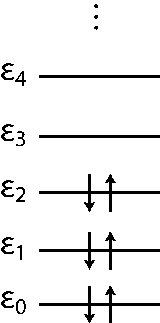
\includegraphics{orbitals.pdf}
  \end{center}
  \caption{\label{fig:orbitals} Illustration of spin-orbitals and a
    Slater determinant of 6 electrons}
\end{figure}




\subsection{Fock space}

The space $L^2_N$ has the
basis consisting of the Slater determinants $\ket{n_0n_1n_2n_3\cdots}$
with in total $N$ occupied orbitals, or $N$ bits set in the binary
representation. The creation operator $c^\dag_\mu$ inserts
a bit in position $\mu$ if it is zero, and gives the zero vector if it
was already 1. Similarly, the operator $c_\mu$ turns a bit off, see
Exercise~\ref{exercise:occupation} 

It is natural to consider \emph{Fock space}, the direct \emph{sum} of
all $L^2_N$:
\begin{equation}
  \mathscr{F} = \bigoplus_{N=0}^\infty L^2_N.
\end{equation}
By definition, $\braket{\vec{\mu}|\vec{\nu}} = 0$ if $\vec{\nu}$ and
$\vec{\mu}$ have different number of particles, i.e., different number
of occupied single-particle functions.

Thus
\begin{equation}
  \braket{0_0 0_1 1_2 0_3 0_4 0_5 0000 \cdots|1_0 1_1 0_2 0_3 0_4 1_5 0000 \cdots} = 0
\end{equation}
for example, since the number of particles differ in the two
functions. 

Now, $c^\dag_\mu : \mathscr{F} \to \mathscr{F}$ maps entirely inside
$\mathscr{F}$, and similarly with $c_\mu$.

A basis for $\mathscr{F}$ is the set of all $\ket{n_0 n_1 \cdots}$
with arbitrary number of orbital occupied.

The binary number representation is quite useful for computer programs
involving Slater determinants, as easily can be imagined.


A special operator, the number operator:
Let $\nu$ be arbitrary. We have that
\begin{equation}
  c_\nu \ket{n_0 n_1 \cdots} = (-1)^{\#\nu} n_\nu \ket{n_0 n_1 \cdots
    0_\nu \cdots},
\end{equation}
and furthermore that
\begin{equation}
  c^\dag_\nu c_\nu \ket{n_0 n_1 \cdots} = (-1)^{2\#\nu} n_\nu \ket{n_0 n_1 \cdots}.
\end{equation}
Thus,
\begin{equation}
  \sum_{\nu} c^\dag_\nu c_\nu \ket{n_0 n_1 \cdots} = \sum_{\nu} n_\nu
  \ket{n_0 n_1\cdots} = N \ket{n_0 n_1 \cdots}.
\end{equation}
Therefore, we define
\begin{equation}
  \hat{N} \equiv \sum_\nu c^\dag_\nu c_nu.
\end{equation}
This operator extracts the number of fermions in a state $\ket{\Psi}$
in the sense that for any $\ket{\Psi} \in \mathscr{F}$, $\hat{N}\ket{\Psi} =
N\ket{\Psi}$ if and only if $\ket{\Psi} \in L^2_N$. 

\subsection{Truncated bases}

For ``physical'' particles, the Hilbert space is infinite
dimensional. But, as we have seen in exercises, especially
Exercise~\ref{exercise:finite}, we can select \emph{a few}
single-particle functions $\phi_\mu$, and construct Slater
determinants out of these. These will be finite in number.

From a mathematical perspective, we can consider these finite
single-particle functions to define a single-particle space on their
own:
\begin{equation}
  V_1 = \operatorname{span}\{\phi_1,\cdots,\phi_L\} \subset L^2(X).
\end{equation}
Thus, $\psi\in V_1$ means
\[ \psi(x) = \sum_{\mu=1}^L \psi_\mu \phi_\mu(x). \]
Having selected the finite basis, we obtain for different $N$ a Slater
determinant basis, spanning $V_N \subset L^2(X^N)_\text{AS}$.

Clearly, as we have only $L$ single-particle functions available, we
cannot create more than $N$ particles from vacuum without getting at
least one repeated creation operator, i.e., we must have $L \geq N$ to
have nonzero dimension. The general dimension is $\dim(V_N) =
\binom{L}{N}$.

In computational settings, the truncation of the inifite basis into a
finite one is almost universally done. Of, course, we can only
numerically diagonalize a finite matrix! But we would still like the
basis to be as large as possible to achieve the greatest accuracy. At
least intuitively, we expect that as we include more and more
single-particle functions, the numerical results will approach the
exact result. Under mild assumptions on the basis set and the
Hamiltonian under consideration, this is in fact true. 

Sometimes, the finite truncation is done after a detailed
consideration of the \emph{physics} of the system. This can give
considerable physical insight, giving great explanatory power to the
second quantized picture. As an example, take the physical explanation
of the principles of a \emph{laser}. (See for example
\url{https://en.wikipedia.org/wiki/Population_inversion}.) Another
example is the \emph{Hubbard model} from solid-state physics, see for example
\url{https://en.wikipedia.org/wiki/Hubbard_model}. 


\begin{exercise}\label{exercise:finite} [Note: This exercise has been
  updated since it was given as a weekly exercise.]

  Let $\phi_\mu$, $\mu=1,2,\cdots,6$ be given orthonormal
  single-particle functions.

  \begin{enumerate}
    \item[a)]
      Using the $\ket{\mu_1,\cdots,\mu_N}$ notation, write down a basis
  for the finite dimensional subspace of $L^2(X^N)_\text{AS}$ for
  $N=2$, $N=3$ and 
  $N=4$, that you can construct using the given single-particle funcitons. (Make sure
  you include only linearly independent Slater determinants.)
  \item[b)]
  Can you construct a Slater determinant for $N=10$ particles using
  the given $\phi_\mu$?

  \item[c)] Using the occupation number notation $\ket{n_1 n_2 \cdots n_6}$
  notation, write down a basis for the same spaces as in exercise a).

  \item[c)] What is the dimension of the subspace of Fock space you can
  create with the $6$ single-particle functions?

  \item[e)] Assume that you have $L$ orbitals instead of just $6$. What is
  the dimension of the $N$-particle spaces you can build? What is the
  dimension of the Fock space you can build?
\end{enumerate}
\end{exercise}

\begin{exercise}[Note: This exercise has been
  updated since it was given as a weekly exercise.]

  Consider the following picture:
  \begin{center}
    \begin{tikzpicture}
      \draw[thick] (0,0) -- (2,0) node[anchor=west] {$\phi_0$};
      \draw[thick] (0,1) -- (2,1) node[anchor=west] {$\phi_1$};
      \draw[thick] (0,2) -- (2,2) node[anchor=west] {$\phi_2$};
      \draw[thick] (0,3) -- (2,3) node[anchor=west] {$\phi_3$};
      \fill (1,0) circle (0.15);
    \end{tikzpicture}
  \end{center}
  We have four horizontal lines, each representing a single-particle
  function $\phi_\mu$. The circle represents an occupied
  single-particle function, i.e., the Slater determinant $\ket{0}$.

  \begin{enumerate}
  \item[a)] In a similar fashion as the the above picture, draw a
    pictures of \emph{all} the distinct Slater determinants you can
    create using the four single-particle functions. Make sure you
    consider all possible particle numbers. Caption each picture with
    the corresponding $\ket{\mu_1\mu_2\cdots\mu_N}$.
\end{enumerate}

We now consider electrons. Consider \emph{4 spin-orbitals}
$\varphi_p(\vec{r})$, i.e., $8$ spin-orbitals
$\phi_\mu(\vec{r},\sigma)$. The corresponding diagram for the Slater
determinant $\ket{0\uparrow,0\downarrow}$ is:
  \begin{center}
    \begin{tikzpicture}
      \draw[thick] (0,0) -- (2,0) node[anchor=west] {$\varphi_0$};
      \draw[thick] (0,1) -- (2,1) node[anchor=west] {$\varphi_1$};
      \draw[thick] (0,2) -- (2,2) node[anchor=west] {$\varphi_2$};
      \draw[thick] (0,3) -- (2,3) node[anchor=west] {$\varphi_3$};
      \node at (0.5,0) {\Large$\uparrow$};
      \node at (1.5,0) {\Large$\downarrow$};
    \end{tikzpicture}
  \end{center}
  Each level now can hold 2 electrons, spin up and spin down. 

  \begin{enumerate}
  \item[b)] Draw all possible $2$-electron Slater determinants. Mark those
    that have total spin projection 0.
  \item[c)] Consider the one-body operator given by
    \[ \hat{H}_0 = \sum_{p} \epsilon_p (c^\dag_{p\uparrow} c_{p\uparrow}
  + c^\dag_{p\downarrow} c_{p\downarrow}). \]  
  Here, $\epsilon_p$ are numbers such that $\epsilon_1 < \epsilon_2 < \cdots$.
  In first quantization,
  \[ \hat{H}_0 = \sum_{i=1}^N \hat{h}(i). \] Write down the matrix of
  the (single-electron) operator $\hat{h}$ in the spin-orbital basis
  $\{\phi_{p\sigma}\}$ and find its eigenfunctions. Interpret the
  spin-orbital diagram in terms of your results. Find the $N=4$ ground
  state of $\hat{H}_0$, and draw a picture of it.
\end{enumerate}
\end{exercise}

\section{Representation of operators}

\subsection{What we will prove}


In this section, we shall demonstrate the following representation of
one-body operators:
\begin{equation}
  \hat{H}_0 = \sum_{i=1}^N \hat{h}(i) = \sum_{\mu\nu}
  \braket{\mu|\hat{h}|\nu} c^\dag_\mu
  c_\nu.\label{eq:onebody-operator-rep} 
\end{equation}
Note that the last expression \emph{does not contain $N$ explicitly}.
Here, note that $\ket{\mu}$ is a single-particle function -- it is the
``Slater determinant'' $\phi_\mu(x_1)$. The number
$\braket{\mu|\hat{h}|\nu}$ is the matrix element of the
single-particle operator $\hat{h}$ in the given one-particle basis,
\begin{equation}
  \braket{\mu|\hat{h}|\nu} = \int dx \phi_\mu(x)^* \hat{h}
  \phi_\nu(x).
\end{equation}
Eq.~\eqref{eq:onebody-oper-rep} gives a nice image of how
$\hat{H_0}$ acts on a basis function: each term in the sum manipulates
the Slater determinant's occupied orbitals and weighs it with a matrix
element. Simple, and not at all obvious from the ``single quantized
form''. 

We shall also prove the following formula for the two-body operator:
\begin{equation}
  \hat{W} = \sum_{(i,j)}^N \hat{w}(i,j) = \tfrac{1}{2} \sum_{\mu\nu\alpha\beta}
  w^{\alpha\beta}_{\mu\nu} c^\dag_\mu c^\dag_\nu
  c_\beta c_\alpha, \label{eq:twobody-operator-rep} 
\end{equation}
where the ordering of the annihilation operators should be
noted. Here,
\begin{equation}
  w^{\mu\nu}_{\alpha\beta} = \int
  dx_1\int dx_2 \phi_\mu(x_1)^*\phi_\nu(x_2)^* w(x_1,x_2)
  \phi_\alpha(x_1)\phi_\beta(x_2) \label{eq:twobody-matelem}
\end{equation}
is a matrix element using tensor product two-body functions,
\emph{not} Slater determinants. Using Slater determinant matrix
elements we in fact have a similar expansion,
\begin{equation}
  \hat{W} = \tfrac{1}{4} \sum_{\mu\nu\alpha\beta}
  \braket{\mu\nu|\hat{w}|\alpha\beta} c^\dag_\mu c^\dag_\nu
  c_\beta c_\alpha, \label{eq:twobody-operator-rep-as} 
\end{equation}
where thus the matrix elements \emph{are antisymmetric}, computed as a matrix
element using two-body Slater determinants.

A word of warning: notation for two-body matrix elements is notoriouly
varying between sources. Some authors use the notation
$\braket{\phi_\alpha\phi_\beta|\hat{w}|\phi_\mu\phi_\nu}$ for the
matrix element $w^{\alpha\beta}_{\mu\nu}$, which is \emph{not}
antisymmetric. In our case, the notation clashes with the Slater
determinant matrix element, but we will still sin in this respect. Some authors write
$\braket{\phi_\alpha\phi_\beta|\hat{w}|\phi_\mu\phi_\nu}_\text{AS}$
for the anti-symmetric Slater-determinant matrix element (and
sometimes we will too), which is
equal to:
\begin{equation}
  \braket{\phi_\alpha\phi_\beta|\hat{w}|\phi_\mu\phi_\nu}_\text{AS} =
  \braket{\alpha\beta|\hat{w}|\mu\nu} = 
  w^{\alpha\beta}_{\mu\nu} - w^{\alpha\beta}_{\nu\mu}. \label{eq:twobody-matelem-as}
\end{equation}
This can cause some confusion, as the expansions using tensor products
and Slater determinants differ by a factor $2$ \ldots

The proofs given in this section borrow heavily from
\cite{HarrisMonkhorstFreeman}.


\begin{lemma}\label{lemma:replacement}
  Let $\ket{\mu_1\mu_2\cdots\mu_N}$ be a Slater determinant built from
  orthonormal single-particle functions $\phi_\mu$, no
  particular ordering assumed. The
  operator $c^\dag_\nu c_\alpha$ replaces $\phi_\alpha$ with $\phi_\nu$ (or
  gives zero of $\alpha$ is not present in $\vec{\mu}$),  with no sign change. 

  Similarly, $c^\dag_{\nu_1} c^\dag_{\nu_2} c_{\alpha_2} c_{\alpha_1}$
  replaces $\alpha_1$ with $\nu_1$, and $\alpha_2$ with $\nu_2$, or gives
  zero if one of $\alpha_1$ or $\alpha_2$ is not present in $\vec{\mu}$.
\end{lemma}

\begin{exercise}
  Prove the lemma.
\end{exercise}

\subsection{One-body operators}

We prove Eq.~\eqref{eq:onebody-operator-rep} by showing that the
actions of the left- and right-hand sides on an arbitrary Slater
determinant agree. Let therefore
$\{\phi_\mu\}$ be a single-particle basis as usual.


Consider the action of $\hat{H}_0 = \sum_i \hat{h}(i)$ on an arbitrary
Slater determinant:
\begin{equation}
  \begin{split}
    \hat{H}_0 \ket{\phi_{\mu_1}, \phi_{\mu_2}, \cdots, \phi_{\mu_N}}
    &= \frac{1}{\sqrt{N!}} \left(\sum_i \hat{h}(i)\right) \sum_\sigma (-1)^{|\sigma|}
    \hat{P}_\sigma \phi_{\nu_1}(x_1)\cdots \phi_{\nu_N}(x_N) \\
    &= \frac{1}{\sqrt{N!}} \sum_\sigma (-1)^{|\sigma|}
    \hat{P}_\sigma \left(\sum_i \hat{h}(i)\right)
    \phi_{\nu_1}(x_1)\cdots \phi_{\nu_N}(x_N) \\
    & = \ket{(\hat{h}\phi_{\nu_1}), \phi_{\nu_2},\cdots,\phi_{\nu_N}}
    + \ket{\phi_{\nu_1}, (\hat{h}\phi_{\nu_2}),\cdots,\phi_{\nu_N}} +
    \cdots + \ket{\phi_{\nu_1},\phi_{\nu_2},\cdots,(\hat{h}\phi_{\nu_N})} 
\end{split}
\end{equation}
Here, we used that $\hat{P}_\sigma$ commutes with $\hat{H}_0$.

Consider the operator $\hat{h}$ acting on a single-particle
function $\phi_\mu$. The result, $\psi$, can be expanded in the basis:
\begin{equation}
  \psi(x) = \hat{h}\phi_\mu(x) = \sum_\nu \phi_\nu(x)
  \braket{\nu|\hat{h}|\mu}.
\end{equation}
We insert this expansion:
\begin{equation}
  \begin{split}
    \hat{H}_0 \ket{\phi_{\mu_1}, \phi_{\mu_2}, \cdots, \phi_{\mu_N}}
    & = \ket{(\hat{h}\phi_{\nu_1}), \phi_{\nu_2},\cdots,\phi_{\nu_N}}
    + \ket{\phi_{\nu_1}, (\hat{h}\phi_{\nu_2}),\cdots,\phi_{\nu_N}} +
    \cdots +
    \ket{\phi_{\nu_1},\phi_{\nu_2},\cdots,(\hat{h}\phi_{\nu_N})} \\
    & = \sum_{\nu} \braket{\nu|\hat{h}|\mu_1}
    \ket{\nu\mu_2,\cdots,\mu_N} + 
    \sum_{\nu} \braket{\nu|\hat{h}|\mu_2}
    \ket{\mu_1\nu\mu_3,\cdots,\mu_N} + \cdots +
    \sum_{\nu} \braket{\nu|\hat{h}|\mu_N}
    \ket{\mu_1\mu_2,\cdots,\nu}
  \end{split}
\end{equation}
Now, we note that
\begin{equation}
  \ket{\mu_1,\cdots,\mu_{j-1}\nu\mu_{j+1}\cdots \mu_N} = c^\dag_\nu
  c_{\mu_j} \ket{\mu_1,\cdots,\mu_N},
\end{equation}
which we plug in:
\begin{equation}
  \begin{split}
    \hat{H}_0 \ket{\phi_{\mu_1}, \phi_{\mu_2}, \cdots, \phi_{\mu_N}} 
    & = \sum_{\nu} \braket{\nu|\hat{h}|\mu_1}
    \ket{\nu\mu_2,\cdots,\mu_N} + 
    \sum_{\nu} \braket{\nu|\hat{h}|\mu_2}
    \ket{\mu_1\nu\mu_3,\cdots,\mu_N} + \cdots +
    \sum_{\nu} \braket{\nu|\hat{h}|\mu_N}
    \ket{\mu_1\mu_2,\cdots,\nu} \\ 
    & =\left[\sum_{\nu} \braket{\nu|\hat{h}|\mu_1} c^\dag_\nu c_{\mu_1}
    + 
    \sum_{\nu} \braket{\nu|\hat{h}|\mu_2} c^\dag_\nu c_{\mu_2}
     + \cdots +
    \sum_{\nu} \braket{\nu|\hat{h}|\mu_N} c^\dag_\nu c_{\mu_N}\right]
    \ket{\mu_1,\cdots,\mu_N}.
  \end{split}
\end{equation}
Finally, we note that $c_\mu \ket{\mu_1\cdots\mu_N} = 0$ whenever
$\mu\notin\vec{\mu}$, so we may extend the summation over $\mu_j$ to
all of $\mu$, resulting in:
\begin{equation}
  \begin{split}
    \hat{H}_0 \ket{\phi_{\mu_1}, \phi_{\mu_2}, \cdots, \phi_{\mu_N}} 
    & =\left[\sum_{\nu} \braket{\nu|\hat{h}|\mu_1} c^\dag_\nu c_{\mu_1}
    + 
    \sum_{\nu} \braket{\nu|\hat{h}|\mu_2} c^\dag_\nu c_{\mu_2}
     + \cdots +
    \sum_{\nu} \braket{\nu|\hat{h}|\mu_N} c^\dag_\nu c_{\mu_N}\right]
    \ket{\mu_1,\cdots,\mu_N} \\
 & = \sum_{\mu\nu} \braket{\nu|\hat{h}|\mu} c^\dag_\nu c_\mu \ket{\mu_1,\cdots,\mu_N}.
  \end{split}
\end{equation}
Since $\ket{\mu_1,\cdots,\mu_N}$ was an arbitrary Slater determinant,
we have proven Eq.~\eqref{eq:onebody-operator-rep}.


\subsection{Two-body operators}

The operator $\hat{W} = \sum_{i<j} \hat{w}(i,j)$ is a two-body
operator. The operator $\hat{w}(1,2)$ is thus an operator on
$L^2(X^2)$ that is completely characterized by its action on a basis:
the tensor products $\phi_{\mu_1}(x_1)\phi_{\mu_2}(x_2)$. Thus,
\begin{equation}
  \hat{w}(1,2)\phi_{\mu_1}(x_1)\phi_{\mu_2}(x_2) = \sum_{\nu_1\nu_2}
  w^{\nu_1\nu_2}_{\mu_1\mu_2} \phi_{\nu_1}(x_1) \phi_{\nu_2}(x_2),\label{eq:0}
\end{equation}
where the matrix elements $w^{\nu_1\nu_2}_{\mu_1\mu_2}$ are given by
the formula~\eqref{eq:twobody-matelem}. There is nothing special about
the indices $(1,2)$, it may just as well be $(i,j)$. Note also the
symmetry property
\[ w^{\nu_1\nu_2}_{\mu_1\mu_2} = w^{\nu_2\nu_1}_{\mu_2\mu_1} .\]


As for the one-body case, $\hat{W}$ commutes with $\hat{P}_\sigma$,
and we get, using Eq.~\eqref{eq:0},
\begin{equation}
  \begin{split}
    \hat{W}\ket{\phi_{\mu_1}\cdots\phi_{\mu_N}} &= \frac{1}{\sqrt{N!}}
    \sum_\sigma (-1)^{|\sigma|} \hat{P}_\sigma \left[\sum_{i<j}
      \hat{w}(i,j)\phi_{\mu_1}(x_1)\cdots\phi_{\mu_N}(x_N) \right] \\ 
    & = \frac{1}{\sqrt{N!}}
    \sum_\sigma (-1)^{|\sigma|} \hat{P}_\sigma \left[\sum_{i<j}
      \hat{w}(i,j)\phi_{\mu_1}(x_1)\cdots\phi_{\mu_N}(x_N) \right] \\ 
    &=\frac{1}{\sqrt{N!}} \sum_\sigma (-1)^{|\sigma|} \hat{P}_\sigma
    \left[ \sum_{i<j} \sum_{\nu_1\nu_2} w^{\nu_1\nu_2}_{\mu_i\mu_j}
      \phi_{\mu_1} \cdots \phi_{\nu_1}(x_i) \cdots \phi_{\nu_2}(x_j)
      \cdots \phi_{\mu_N}(x_N) \right] \\
    & = \sum_{i<j} \sum_{\nu_1\nu_2}
    w^{\nu_1\nu_2}_{\mu_i\mu_j}
    \ket{\phi_{\mu_1}\cdots\phi_{\nu_1}\cdots\phi_{\nu_2}\cdots
      \phi_{\mu_N}} \\
    & = \sum_{i<j} \sum_{\nu_1\nu_2}
    w^{\nu_1\nu_2}_{\mu_i\mu_j}
    c^\dag_{\nu_1}c^\dag_{\nu_2}
    c_{\mu_j}c_{\mu_i}\ket{\phi_{\mu_1}\cdots\phi_{\mu_N}}.
  \end{split}
\end{equation}
Here, we used Lemma~\ref{lemma:replacement} about replacement behaviour of the $c^\dag
c^\dag c c$ product. We are currently summing over $\mu_i$ and
$\mu_j$, such that $i<j$. Including $i=j$ gives zero contribution
(why?), and including $j>i$ gives equal contribution:
\begin{equation}
  \begin{split}
    &\sum_{i<j} \sum_{\nu_1\nu_2}
    w^{\nu_1\nu_2}_{\mu_i\mu_j}
    c^\dag_{\nu_1}c^\dag_{\nu_2}
    c_{\mu_j}c_{\mu_i}\ket{\phi_{\mu_1}\cdots\phi_{\mu_N}} = 
    -\sum_{i<j} \sum_{\nu_1\nu_2}
    w^{\nu_1\nu_2}_{\mu_i\mu_j}
    c^\dag_{\nu_1}c^\dag_{\nu_2}
    c_{\mu_i}c_{\mu_j}\ket{\phi_{\mu_1}\cdots\phi_{\mu_N}} \\
    &=  \sum_{i<j} \sum_{\nu_1\nu_2}
    w^{\nu_1\nu_2}_{\mu_i\mu_j}
    c^\dag_{\nu_2}c^\dag_{\nu_1}
    c_{\mu_i}c_{\mu_j}\ket{\phi_{\mu_1}\cdots\phi_{\mu_N}} 
    =  \sum_{j<i} \sum_{\nu_1\nu_2}
    w^{\nu_1\nu_2}_{\mu_j\mu_i}
    c^\dag_{\nu_2}c^\dag_{\nu_1}
    c_{\mu_j}c_{\mu_i}\ket{\phi_{\mu_1}\cdots\phi_{\mu_N}} \\
    &=  \sum_{j<i} \sum_{\nu_2\nu_1}
    w^{\nu_2\nu_1}_{\mu_j\mu_i}
    c^\dag_{\nu_1}c^\dag_{\nu_2}
    c_{\mu_j}c_{\mu_i}\ket{\phi_{\mu_1}\cdots\phi_{\mu_N}} 
    =  \sum_{j<i} \sum_{\nu_2\nu_1}
    w^{\nu_1\nu_2}_{\mu_i\mu_j}
    c^\dag_{\nu_1}c^\dag_{\nu_2}
    c_{\mu_j}c_{\mu_i}\ket{\phi_{\mu_1}\cdots\phi_{\mu_N}} 
  \end{split}
\end{equation}
Here, we used the anticommutators and symmetry of the matrix elements.
Assembling the two contributions,
\begin{equation}
  \hat{W} \ket{\phi_{\mu_1}\cdots\phi_{\mu_N}} = \frac{1}{2} \sum_{ij} \sum_{\nu_2\nu_1}
    w^{\nu_1\nu_2}_{\mu_i\mu_j}  c^\dag_{\nu_1}c^\dag_{\nu_2}
    c_{\mu_j}c_{\mu_i}\ket{\phi_{\mu_1}\cdots\phi_{\mu_N}} .
\end{equation}
We note that the sum over $ij$ is really a sum over two occupied
orbitals $\mu_i$ and $\mu_j$. We can therefore extend the sum to all
unoccupied orbitals as well, since $c_{\alpha}\ket{\vec{\mu}}$ gives zero contributions
for such orbitals. Thus, Eq.~\eqref{eq:twobody-operator-rep} is
proven.

We leave the proof of the antisymmetrized version as an exercise.
\begin{exercise}
  Prove Eq.~\eqref{eq:twobody-operator-rep-as}. Start with showing
  Eq.~\eqref{eq:twobody-matelem-as}.
\end{exercise}



\begin{exercise}\label{exercise:diagonal-matrix-elements} % From MHJ
  a) Let $\hat{F} = \sum_{i=1}^N \hat{f}(i)$ be a first-quantization
  operator. Write down the second-quantized form of this operator. Let
  $\hat{G} = \sum_{i<j} \hat{g}(i,j)$ be a general two-body operator,
  where $\hat{g}(1,2) = \hat{g}(2,1)$. Write down the second-quantized
  form.

  b) Using the fundamental anticommutator relations, compute the matrix element
  \[ \braket{\mu_1\mu_2|\hat{F}|\mu_1\mu_2} \]

  c) Using the fundamental anticommutator relations, compute the matrix element
  \[ \braket{\mu_1\mu_2\mu_3|\hat{F}|\mu_1\mu_2\mu_3} \]

  d) Using the fundamental anticommutator relations, compute the matrix element
  \[ \braket{\mu_1\mu_2|\hat{G}|\mu_1\mu_2} \]

  e) Using the fundamental anticommutator relations, compute the matrix element
  \[ \braket{\mu_1\mu_2\mu_3|\hat{G}|\mu_1\mu_2\mu_3} \]
  
  f) Compute the matrix element
  \[  \braket{\mu_1,\mu_2,\cdots,\mu_N|\hat{F}|\mu_1,\mu_2,\cdots,\mu_N} \]

  g) Compute the matrix element
  \[  \braket{\mu_1,\mu_2,\cdots,\mu_N|\hat{G}|\mu_1,\mu_2,\cdots,\mu_N} \]
  
\end{exercise}


\begin{exercise}\label{exercise:slater-condon-rules}(Tedious, but very instructive.)
  In this exercise, we prove the so-called \emph{Slater--Condon rules}: the
  explicit expressions of matrix elements of one- and two-body
  operators in a Slater determinant basis.

  We do not assume any particular ordering of the occupied
  single-particle functions considered.

  If you solved Exercise~\ref{exercise:diagonal-matrix-elements}, you
  solved parts of this exercise.

  a) Using the fundamental anticommutator relations, compute
  $\braket{\vec{\mu}|\hat{H}_0|\vec{\mu}}$ and
  $\braket{\vec{\mu}|\hat{W}|\vec{\mu}}$ and prove that
  \begin{align}
    \braket{\vec{\mu}|\hat{H}_0|\vec{\mu}} &= \sum_{i=1}^N
    h^{\mu_i}_{\mu_i}, \\ \braket{\vec{\mu}|\hat{W}|\vec{\mu}} &=
    \sum_{i<j}^N \braket{\mu_i\mu_j|\hat{w}|\mu_i\mu_j}_\text{AS} =
    \frac{1}{2}\sum_{ij} \braket{\mu_i\mu_j|\hat{w}|\mu_i\mu_j}_\text{AS}.
  \end{align}
  
  b) Let $\vec{\nu}$ be equal to $\vec{\mu}$, except for one occupied orbital, i.e.,
  \begin{equation}
    \ket{\vec{\nu}} = c^\dag_{\nu_j} c_{\mu_j} \ket{\vec{\mu}}, \quad
    \nu_j \neq \mu_j.
  \end{equation}
  Using the fundamental anticommutator relations, compute $\braket{\vec{\mu}|\hat{H}_0|\vec{\mu}}$ and
  $\braket{\vec{\mu}|\hat{W}|\vec{\nu}}$, and find
  \begin{align}
    \braket{\vec{\mu}|\hat{H}_0|\vec{\nu}} &= h^{\mu_j}_{\nu_j}, \\
    \braket{\vec{\mu}|\hat{W}|\vec{\nu}} &= \sum_i \braket{\mu_i \mu_j|\hat{w}|\mu_i\nu_j}_\text{AS}.
  \end{align}
  
  c) Let $\vec{\nu}$ be equal to $\vec{\mu}$, except for two indices, i.e.,
  \begin{equation}
    \ket{\vec{\nu}} = c^\dag_{\nu_k} c^\dag_{\nu_j} c_{\mu_j}
    c_{\mu_j} \ket{\vec{\mu}}, \quad j \neq k.
  \end{equation}
  Using the fundamental anticommutator relations, compute
  $\braket{\vec{\mu}|\hat{W}|\vec{\nu}}$ and find
  \begin{align}
    \braket{\vec{\mu}|\hat{H}_0|\vec{\nu}} &= 0, \\
    \braket{\vec{\mu}|\hat{W}|\vec{\nu}} &= \braket{\mu_j \mu_k|\hat{w}|\nu_j\nu_k}_\text{AS}.
  \end{align}
  
  d) Explain that if $\vec{\nu}$ differs from $\vec{\mu}$ in
  \emph{more} than two occupied functions, then
  $\braket{\vec{\mu}|\hat{W}|\vec{\nu}} = 0$.

\end{exercise}



\begin{exercise}%MHJ
 (This exercise adapted from an exercise by Morten Hjorth-Jensen.)

  We will now consider a simple three-level problem, depicted in
  Figure~\ref{fig:exercise-orbitals}.  The single-particle
  states are labelled by the quantum number $p$ and can accomodate up
  to two single particles, viz., every single-particle state is doubly
  degenerate (you could think of this as one state having spin up and
  the other spin down).  We let the spacing between the doubly
  degenerate single-particle states be constant, with value $d$.  The
  first state has energy $d$. There are only three available
  single-particle states, $p=1$, $p=2$ and $p=3$, as illustrated in
  the figure.
\begin{enumerate}
\item[a)] How many two-particle Slater determinants can we construct in this space? 
\item[b)] We limit ourselves to a system with only the two lowest single-particle orbits and two particles, $p=1$ and $p=2$.
We assume that we can write the Hamiltonian as
\[
       \hat{H}=\hat{H}_0+\hat{H}_I,
\]
and that the onebody part of the Hamiltonian with single-particle operator $\hat{h}_0$ has the property
\[
\hat{h}_0\psi_{p\sigma} = p\times d \psi_{p\sigma},
\]
where we have added a spin quantum number $\sigma$. 
We assume also that the only two-particle states that can exist are those where two particles are in the 
same state $p$, as shown by the two possibilities to the left in the figure.
The two-particle matrix elements of $\hat{H}_I$ have all a constant value, $-g$.
\begin{figure}
  \begin{center}
  \begin{tikzpicture}
    \draw[thick] (0,0) node[anchor=east] {$p=1$} -- (2,0);
    \draw[thick] (0,1) node[anchor=east] {$p=2$} -- (2,1);
    \draw[thick] (0,2) node[anchor=east] {$p=3$} -- (2,2);
    \fill (0.5,0) circle (0.15);
    \fill (1.5,0) circle (0.15);
  \begin{scope}[xshift=3cm]
    \draw[thick] (0,0) node[anchor=east] {$$} -- (2,0);
    \draw[thick] (0,1) node[anchor=east] {$$} -- (2,1);
    \draw[thick] (0,2) node[anchor=east] {$$} -- (2,2);
    \fill (0.5,1) circle (0.15);
    \fill (1.5,1) circle (0.15);
  \end{scope}
  \begin{scope}[xshift=6cm]
    \draw[thick] (0,0) node[anchor=east] {$$} -- (2,0);
    \draw[thick] (0,1) node[anchor=east] {$$} -- (2,1);
    \draw[thick] (0,2) node[anchor=east] {$$} -- (2,2);
    \fill (0.5,0) circle (0.15);
    \fill (1.5,2) circle (0.15);
  \end{scope}
  \begin{scope}[xshift=9cm]
    \draw[thick] (0,0) node[anchor=east] {$$} -- (2,0);
    \draw[thick] (0,1) node[anchor=east] {$$} -- (2,1);
    \draw[thick] (0,2) node[anchor=east] {$$} -- (2,2);
    \fill (0.5,1) circle (0.15);
    \fill (1.5,2) circle (0.15);
  \end{scope}
  \end{tikzpicture}
\end{center}
\caption{Schematic plot of the possible single-particle levels with double degeneracy.
The filled circles indicate occupied particle states.
The spacing between each level $p$ is constant in this picture. We show some possible two-particle states.\label{fig:exercise-orbitals}}
\end{figure}
Show then that the Hamiltonian matrix can be written as 
\[
\left(\begin{array}{cc}2d-g &-g \\
-g &4d-g \end{array}\right),
\]
and find the eigenvalues and eigenvectors.  What is mixing of the state with two particles in $p=2$ 
to the wave function with two-particles in $p=1$? Discuss your results in terms of a linear combination
of Slater determinants.  \\
\item[c)] Add the possibility that the two particles can be in the state with $p=3$ as well and find the Hamiltonian
matrix, the eigenvalues and the eigenvectors. We still insist that we only have two-particle states composed of two particles being in the same
level $p$. You can diagonalize numerically your $3\times 3$ matrix.\newline\newline
This simple model catches several birds with a stone. It demonstrates how we can build linear combinations
of Slater determinants and interpret these as different admixtures to a given state. It represents also the way we are going to interpret these contributions.  The two-particle states above $p=1$ will be interpreted as 
excitations from the ground state configuration, $p=1$ here.  The reliability of this ansatz for the ground state, 
with two particles in $p=1$,
depends on the strength of the interaction $g$ and the single-particle spacing $d$.
Finally, this model is a simple schematic ansatz for studies of pairing correlations and thereby superfluidity/superconductivity  
in fermionic systems. 
\end{enumerate}


\end{exercise}

\section{Wick's Theorem}

Supporting material for this section is Shavitt/Bartlett Ch.~3,
Gross/Runge/Heinonen Ch.~19.

\subsection{A sort of summary and motivation}

Let us take a look at what we have so far. In the preceeding sections, 
we introduced a collection of tools for describing (1) many-fermion
states in many-particle Hilbert space, and (2) second-quantization
language for expressing these states and, importantly, the
quantum-mechanical Hamiltonian.

The quantum mechanical Hilbert space for $N$ fermions is defined
solely in terms of the \emph{configuration space} $X$ of a single
fermion. The Hilbert space of a single particle is $L^2(X)$, the set of square
integrable single-particle functions $\psi : X \to \CC$. 

Such a space always has an orthonormal basis, say
$\{\phi_\mu\}$. Forming \emph{Slater determinants}
$\ket{\phi_{\mu_1}\phi_{\mu_2}\cdots \phi_{\mu_N}}$, we obtain totally
antisymmetric basis functions for $L^2(X^N)_\text{AS}$. Furthermore,
we defined \emph{Fock space} $\mathscr{F}$,
\[\mathscr{F} = \bigoplus_{N=0}^\infty L^2(X^N)_\text{AS}. \]
Inside the Fock space, \emph{every possible wavefunction of a system
  of some number of fermions exist}. 

%Note that a different configuration space $X$ leads to a different
%Fock space: electrons in $\RR^3$ have a different space than nucleons,
%for example. However, a different choise of single-particle basis
%$\{\phi_\mu\}$ does \emph{not lead to a different Fock space}. It is
%the configuration space $X$ that defines the space of possible states.

Given a wavefunction $\ket{\Psi_N} \in \mathscr{F}$, it could be
expanded in Slater determinants,
\begin{equation}
  \ket{\Psi_N} = \sum_{\vec{\mu}}^\sim \ket{\mu_1\cdots\mu_N}
  \braket{\mu_1\cdots\mu_N|\Psi_N}. 
\end{equation}
Here, the subscript $N$ only indicates that we know the number of
particles.  The notation $\ket{\mu_1\cdots\mu_N}$ indicates that a
certain single-particle basis $\{\phi_\mu\}$ has been chosen, since we
only list the indices $\mu_j$.  Each determinant can be constructed
from vacuum using \emph{creation operators} $c^\dag_\mu$ (these, of
course, depend on the basis),
\begin{equation}
  \ket{\mu_1\cdots\mu_N} = c^\dag_{\mu_1} c^\dag_{\mu_2} \cdots
  c^\dag_{\mu_N} \ket{-}.
\end{equation}

Finally, we found expressions for one- and two-body operators in terms
of creation and annihilation operators:
\begin{align}
  \hat{H}_0 &= \sum_{\mu\nu} \braket{\mu|\hat{h}|\nu} c^\dag_\mu c_\nu
  \\
  \hat{W} &= \frac{1}{4} \sum_{\substack{\nu_1\nu_2\\\mu_1\mu_2}}
  \braket{\mu_1\mu_2|\hat{w}|\nu_1\nu_2} c^\dag_{\mu_1} c^\dag_{\mu_2}
  c_{\nu_2} c_{\nu_1}.
\end{align}
We claimed that these expressions simplify our life a lot. 

Our life goal in this context is to solve the (time-independent)
Schr\"odinger equation,
\begin{equation}
  (\hat{H}_0 + \hat{W})\ket{\Psi_N} = E \ket{\Psi_N}.
\end{equation}
This expression equates two elements (functions) in Hilbert
space. These functions are equal if and only if their basis
projections are equal. Thus, we expand $\ket{\Psi_N}$ in the basis,
and similarly with the left-hand side $\hat{H}\ket{\Psi_N}$:
\begin{equation}
  \sum_{\vec{\mu}}^\sim \bra{\nu_1\cdots\nu_N} (\hat{H}_0 + \hat{W})
  \ket{\mu_1\cdots \mu_N} \braket{\mu_1\cdots\mu_N|\Psi_N} = E \braket{\nu_1\cdots\nu_N|\Psi_N}.
\end{equation}
Defining the vector $\mathsf{C}_{\vec{\mu}} = \braket{\vec{\mu}|\Psi_N}$ and
the matrix $\mathsf{H}_{\vec{\nu},\vec{\mu}} =
\braket{\vec{\nu}|\hat{H}|\vec{\mu}}$, we see that we have a
\emph{matrix eigenvalue problem}
\begin{equation}
  \mathsf{H}\mathsf{C} = E\mathsf{C}. \label{eq:SE-matrix}
\end{equation}

Remark: this equation is (usually) infinite-dimensional, and from a strict
mathematical point of view, this must really be carefully defined. But
in this course, it is sufficient to think of this as a standard matrix
eigenvalue problem.

Ok, so we have a way of describing \emph{vectors} $\ket{\Psi_N}$ and
the operators $\hat{H}_0$ etc. But if we actually want to \emph{solve}
Eq.~\eqref{eq:SE-matrix}, we need to compute the matrix
elements\footnote{On a computer, we need to truncate the basis to
  obtain a finite-dimensional matrix eigenvalue problem. Only for very
  small problems will one actually compute the matrix itself, because
  that is quite expensive. Rather, one computes the
  \emph{matrix-vector product} $\hat{H}\ket{\vec{\mu}}$.}

\begin{equation}
  \mathsf{H}_{0,\vec{\nu},\vec{\mu}} =
  \braket{\vec{\mu}|\hat{H}_0|\vec{\mu}} = \sum_{\mu\nu}
  \braket{\mu|\hat{h}|\nu} \bra{-} c_{\nu_N} c_{\nu_{N-1}} \cdots
  c_{\nu_1} c^\dag_\mu c_\nu c^\dag_{\mu_1} c^\dag_{\mu_2}\cdots
  c^\dag_{\mu_N} \ket{-}
\end{equation}
and similarly
\begin{equation}
  \mathsf{W}_{\vec{\nu},\vec{\mu}} =
  \braket{\vec{\mu}|\hat{W}|\vec{\mu}} = \frac{1}{4}
  \sum_{\substack{\alpha_1\alpha_2\\\beta_1\beta_2}} 
  \braket{\alpha_1\alpha_2|\hat{w}|\beta_1\beta_2} \bra{-} c_{\nu_N} c_{\nu_{N-1}} \cdots  c_{\nu_1} c^\dag_{\alpha_1} c^\dag_{\alpha_2} c_{\beta_2} c_{\beta_1} c^\dag_{\mu_1} c^\dag_{\mu_2}\cdots  c^\dag_{\mu_N} \ket{-}
\end{equation}
Notice that we used
\begin{equation}
  \ket{\mu_1\cdots\mu_N} = c^\dag_{\mu_1}\cdots c^\dag_{\mu_N}\ket{-}
\end{equation}
and, by taking the adjoint,
\begin{equation}
  \bra{\mu_1\cdots\mu_N} = \bra{-} c_{\mu_N} \cdots c_{\mu_1}.
\end{equation}
Observe that the order of the annihilation operators is the reverse of
the order of the creation operators.

The number $\bra{-} c^{(\dag)} c^{(\dag)} \cdots c^{(\dag)}\ket{-}$ is
referred to a \emph{vacuum expectation value}, and the problem of
computing matrix elements is basically reduced to computing these.

Let us consider an example, and compute a typical vacuum expectation
value occuring in the $\hat{H}_0$ matrix element:
\begin{equation}
  A = \braket{\nu_1\nu_2|c^\dag_\alpha c_\beta|\mu_1\mu_2} =
  \bra{-}c_{\nu_2} c_{\nu_1} c^\dag_\alpha c_\beta c^\dag_{\mu_1}
  c^\dag_{\mu_2} \ket{-}.
\end{equation}
Now, how are we going to approach this problem? Recall the
anticummutation relations,
\begin{gather}
  c_\alpha c^\dag_\beta + c^\dag_\beta c_\alpha = \delta_{\alpha\beta}\\
  c_\alpha c_\beta + c_\beta c_\alpha = 0\\\intertext{and}
  c^\dag_\alpha c^\dag_\beta + c^\dag_\beta c^\dag_\alpha = 0.
\end{gather}
So, we can ``flip'' two creation or annihilation operators adjacent to
each other and compensate with a $-$ sign. We can ``flip'' an
annihilation and creation operator by a $-$ sign, \emph{but} we have
to ``pay a price'' in the form of a Kronecker delta, an additional
term. However, this additional term has two less creation and
annihilation operators.

In this way, we can systematically move the annihilation operators
\emph{to the right}, and the creation operators \emph{to the
  left}, possibly inserting kronecker deltas and generating new terms
with fewer operators. But when the annihilation operators are to the right they
give zero contribution since $c_\alpha\ket{-}= 0$.

Let us see this in practice, and first remove one pair of creation and
annihilation operators:
\begin{equation}
  \begin{split}
    A &= \bra{-}c_{\nu_2} c_{\nu_1} c^\dag_\alpha c_\beta c^\dag_{\mu_1}
    c^\dag_{\mu_2} \ket{-} = \bra{-}c_{\nu_2} c_{\nu_1} c^\dag_\alpha
    (\delta_{\beta\mu_1} - c^\dag_{\mu_1} c_\beta) c^\dag_{\mu_2}
    \ket{-} \\
    & = \delta_{\beta\mu_1}\bra{-}c_{\nu_2} c_{\nu_1} c^\dag_\alpha
    c^\dag_{\mu_2} \ket{-} - \bra{-}c_{\nu_2} c_{\nu_1} c^\dag_\alpha
    c^\dag_{\mu_1} c_\beta c^\dag_{\mu_2} \ket{-} \\
    & = \delta_{\beta\mu_1}\bra{-}c_{\nu_2} c_{\nu_1} c^\dag_\alpha
    c^\dag_{\mu_2} \ket{-} - \bra{-}c_{\nu_2} c_{\nu_1} c^\dag_\alpha
    c^\dag_{\mu_1} (\delta_{\beta\mu_2} - c^\dag_{\mu_2} c_\beta)
    \ket{-} \\
    & = \delta_{\beta\mu_1}\bra{-}c_{\nu_2} c_{\nu_1} c^\dag_\alpha
    c^\dag_{\mu_2} \ket{-} - \delta_{\beta\mu_2}\bra{-}c_{\nu_2} c_{\nu_1} c^\dag_\alpha
    c^\dag_{\mu_1} \ket{-}.
  \end{split}
\end{equation}
We continue:
\begin{equation}
  \begin{split}
    A &= \delta_{\beta\mu_1} \bra{-} c_{\nu_2}(\delta_{\nu_1\alpha} -
    c^\dag_\alpha c_{\nu_1}) c^\dag_{\mu_2}\ket{-} -
\delta_{\beta\mu_2} \bra{-} c_{\nu_2}(\delta_{\nu_1\alpha} -
    c^\dag_\alpha c_{\nu_1}) c^\dag_{\mu_1}\ket{-} \\
     &= \delta_{\beta\mu_1}\delta_{\nu_1\alpha}\bra{-}c_{\nu_2}
     c^\dag_{\mu_2}\ket{-} - \delta_{\beta\mu_1}\bra{-}c_{\nu_2}
       c^\dag_\alpha c_{\nu_1} c^\dag_{\mu_2}\ket{-} - \left( \mu_1
         \leftrightarrow \mu_2\right) .
  \end{split}
\end{equation}
In the last equality, we have indicated that the remaining terms are
generated from the previous ones by exchanging $\mu_1$ and $\mu_2$.

Continuing,
\begin{equation}
  \begin{split}
    A = \delta_{\beta\mu_1}\delta_{\nu_1\alpha}\bra{-}c_{\nu_2}
     c^\dag_{\mu_2}\ket{-} -
     \delta_{\beta\mu_1}\delta_{\nu_1\mu_2}\bra{-}c_{\nu_2}c^\dag_{\alpha}\ket{-}
     + \delta_{\beta\mu_1} \bra{-}c_{\nu_2} c^\dag_\alpha
     c^\dag_{\mu_2} c_{\nu_1}\ket{-} - \left( \mu_1
         \leftrightarrow \mu_2\right) .
  \end{split}
\end{equation}
Only the two first terms are non-vanishing, and we note, for example,
that $\bra{-}c_{\nu_2} c^\dag_{\mu_2}\ket{-} = \braket{\nu_2|\mu_2} =
\delta_{\nu_2\mu_2}$. (We could also use the anticommutator once
more.) This gives:
\begin{equation}
  A = \delta_{\beta\mu_1} \delta_{\nu_1\alpha} \delta_{\nu_2\mu_2} -
  \delta_{\beta\mu_1}\delta_{\nu_1\mu_2}\delta_{\nu_2\alpha} - (
  \mu_1\leftrightarrow\mu_2).
\end{equation}

Yes, our life was made easier by introducing
second-quantiation. However, the matrix elements are still quite hard
to compute. This is where \emph{Wick's theorem} comes in, by giving a
much quicker way of determining the vacuum expectation values.

Observe that the vacuum expectation value \emph{is basis
  independent}. The value only depends on the anticommutator
relations, and these only depended on the orthonormality of
$\{\phi_\mu\}$. So we see that the framework is quite general.

\subsection{Vacuum expectation values}

Consider the computation of a \emph{vacuum expectation value} of a
\emph{string of creation and annihilation operators}:

\begin{equation}
  \bra{-} A_1 A_2 \cdots A_n \ket{-}, \label{eq:vacexp}
\end{equation}
where each of the $A_i$ are one of the $c^\dag_\mu$ or
$c_\mu$. For example, the overlap between two determinants is on this form:
\begin{equation}
  \braket{\mu_1\cdots \mu_N|\nu_1\cdots\nu_N} = \bra{-} c_{\mu_N}
  c_{\mu_{N-1}} \cdots c_{\mu_1} c^\dag_{\nu_1} c^\dag_{\nu_2} \cdots
  c^\dag_{\nu_N} \ket{-}
\end{equation}
Another example is the matrix elements of an operator on second
quantized form, say $\hat{H}_0$:
\begin{equation}
  \braket{\mu_1\cdots \mu_N|\hat{H}_0|\nu_1\cdots\nu_N} =
  \sum_{\mu\nu} \braket{\mu|\hat{h}|\nu} \braket{\mu_1\cdots
    \mu_N|c^\dag_\mu c_\nu|\nu_1\cdots\nu_N}
  \sum_{\mu\nu} \braket{\mu|\hat{h}|\nu} \bra{-}c_{\mu_N} \cdots
  c_{\mu_1} c^\dag_\mu c_\nu c^\dag_{\mu_1}\cdots c^\dag_{\mu_N} \ket{-}.
\end{equation}
The right-hand side is a linear combination of vacuum expectation
values. So we see that having a straightforward way to compute
Eq.~\eqref{eq:vacexp} would be of great help.

Wick's Theorem is what we shall need.

\subsection{Normal ordering and contractions}

\newcommand*{\pr}[1]{\left(#1\right)}
\newcommand*{\fpr}[1]{\left[#1\right]}
\newcommand*{\kpr}[1]{N\left(#1\right)}
\newcommand*{\for}[3]{\langle#1|#2|#3\rangle}
\newcommand{\OP}[1]{{\hat{#1}}}
\newcommand*{\cre}[1]{c^{\dagger}_{#1}}
\newcommand*{\an}[1]{c_{#1}}

In this section, we denote a general string of $n$ creation and
annihilation operators by
\begin{equation}
  A_1 A_2 \cdots A_n, \quad A_i \in \{ c_\mu \} \cup \{ c^\dag_\mu \}.
\end{equation}
Our goal is to find a general procedure of computing the vacuum
expectation value
\begin{equation}
  \braket{-|A_1A_2\cdots A_n|-}.
\end{equation}
Note that this expectation value only depends on the \emph{orthogonality} of the
single-particle functions, not on the functions themselves. I.e., the
value of the vacuum expectation value can be computed solely from the
anticummutator relations (\ref{eq:anticommutator-relations}).

The procedure we develop is based on \emph{Wick's Theorem}, to be stated and
proven.  Wick's theorem is based on two fundamental concepts, namely
$\textit{normal ordering}$ and $\textit{contraction}$. The
normal-ordered product form of an operator string $A_1A_2\cdots A_n$ is
defined as
\begin{align}
  \label{eq:normal-ordering-def}
  N({A}_1{A}_2\cdots{A}_{n-1}{A}_n) &\equiv (-1)^{|\sigma|}
  \fpr{\text{creation operators}}\cdot\fpr{\text{annihilation
      operators}}
\end{align}
Here, $\sigma \in S_n$ denotes a permutation that brings the operator
product to the desired order,
\begin{equation}
  N({A}_1{A}_2\cdots{A}_{n-1}{A}_n) = (-1)^{|\sigma|} A_{\sigma(1)}
  A_{\sigma(2)} \cdots A_{\sigma(n)}.
\end{equation}

Note that the string $A_1\cdots A_n$ and the normal-order product
$N(A_1\cdots A_n)$ is \emph{not} the same operator, since
by reordering creation and annihilation operators we neglect the extra
terms arising from the Kronecker delta in the anti-commutator relation
$\{c_\alpha, c^\dag_\beta\} = \delta_{\alpha\beta}$. If all individual
$A_i$ in fact anticommute, \emph{then} the string and the normal-ordered
string are identical as operators, but usually this is not the case.

Remark: The permutation $\sigma$ in the definition is usually not be unique,
but the normal ordered product \emph{is} unique as operator. Consider for
example
\begin{equation}
   N( c_1 c^\dag_2 c^\dag_3 c_4 ) = (-1)^2 c^\dag_2 c^\dag_3 c_1 c_4. 
\end{equation} 
There are $2\times 2$ possible arrangements of the creation and
annihilation operators that conform to the definition of the
normal-ordered product. But creation and annihilation operators
anticommute among themselves. The permutation sign $(-1)^{|\sigma|}$
in Eq.~\eqref{eq:normal-ordering-def} automatically compensates for
this. Thus,
\begin{equation}
   N( c_1 c^\dag_2 c^\dag_3 c_4 ) = c^\dag_2 c^\dag_3 c_1 c_4 =
   - c^\dag_3 c^\dag_2 c_1 c_4 = c^\dag_3 c^\dag_2 c_4
   c_1 = -c^\dag_2 c^\dag_3 c_4 c_1.
\end{equation}

We define the normal order product of \emph{linear combinations} in
the obvious way:
\begin{equation}
  N(\alpha A_1\cdots A_n + \beta B_1\cdots B_m) = \alpha N(A_1\cdots
  A_n) + \beta N(B_1\cdots B_n).
\end{equation}

Mathematical aside for the interested reader: $N(\cdot)$ is now defined as a
linear operator on the space of linear combinations of operator
strings. The second-quantized formulas for $\hat{H}_0$,
$\hat{W}$, etc., are examples of such objects. This space of operators
is an example of a \emph{$C^*$-algebra} with unity. An algebra is a vector
space where multiplication is also defined (the product of two
operators is an operator), and roughly speaking the $*$ means that we can form
Hermitian adjoints. The operator algebra is said
to be generated by the $c_\mu$ operators and the unit operator.

A \emph{contraction} between to arbitrary creation and annihilation
operators ${X}$ and ${Y}$ is a special notation for $\braket{-|XY|-}$,
\begin{align}
\contraction[0.5ex]{}{{X}}{}{{Y}}{} 
{X}{Y}  \equiv \for{-}{{X}{Y}}{-}. \label{eq:contr-def}
\end{align}
Thus, the contraction is a \emph{number}. One can easily show (see exercise~\ref{exercise:contraction-relation}), that
\begin{align}
\contraction[0.5ex]{}{{X}}{}{{Y}}{} 
{X}{Y}  = {X}{Y} - N({X}{Y}). \label{eq:contr-def-2}
\end{align}


Let us list all the possible
contractions: 
\begin{subequations}\label{eq:contractions}
\begin{align}
  \contraction[0.5ex]{}{c^\dag_\mu}{}{c^\dag_\nu}{} 
c^\dag_\mu c^\dag_\nu = \braket{-|c^\dag_\mu c^\dag_\nu|-} = 0 \\
  \contraction[0.5ex]{}{c_\mu}{}{c_\nu}{} 
c_\mu c_\nu = \braket{-|c_\mu c_\nu|-} = 0 \\
  \contraction[0.5ex]{}{c^\dag_\mu}{}{c_\nu}{} 
c^\dag_\mu c_\nu = \braket{-|c^\dag_\mu c_\nu|-} = 0 \\
  \contraction[0.5ex]{}{c_\mu}{}{c^\dag_\nu}{} 
c_\mu c^\dag_\nu = \braket{-|c_\mu c^\dag_\nu|-} = \delta_{\mu\nu}. \\
\end{align}
\end{subequations}
As we see, most contractions are actually zero. 

We also define contractions between two operators \emph{inside a normal ordered
  product}. This is defined by first anticommuting the contracted
operators to the front of the product, and then applying Eq.~\eqref{eq:contr-def}.
A contraction between two operators at positions $x$ and $y$ (with $x<y$) in the
string is thus defined by
\begin{align}\label{eq:contraction-inside-normal-order-product}
  N(\contraction[0.5ex]{A_1\cdots}{A_x}{\cdots}{A_y}A_1\cdots A_x \cdots
  A_y \cdots A_n)
  \equiv \pr{-1}^{x+y+1}
  N(\contraction[0.5ex]{}{A_x}{}{A_y} A_x A_y A_1 \cdots
  \strikeout{A_x} \cdots \strikeout{A_y} \cdots A_n)
  = \pr{-1}^{x+y+1}
  \contraction[0.5ex]{}{A_x}{}{A_y} A_x A_y N( A_1 \cdots
  \strikeout{A_x} \cdots \strikeout{A_y} \cdots A_n)
\end{align}
Equivalently, let $\sigma\in S_n$ be a permutation such that
$\sigma(x)=1$ and $\sigma(y)=2$. Then
\begin{equation}
  \begin{split}
    N(\contraction[0.5ex]{A_1\cdots}{A_x}{\cdots}{A_y}A_1\cdots A_x \cdots
    A_y \cdots A_n)
    &\equiv (-1)^{|\sigma|} N(\contraction{}{A_x}{}{A_y}A_x A_y
    A_{\sigma(3)}\cdots A_{\sigma(n)} ) \\
    &= (-1)^{|\sigma|} \contraction{}{A_x}{}{A_y}A_x A_y N(
    A_{\sigma(3)}\cdots A_{\sigma(n)} )
  \end{split}
\end{equation}
(This definition also allows the other operators to be permuted among
themselves. This is of course perfectly acceptable -- the sign of
$\sigma$ accounts for this.)

Thus, the sign factor $(-1)^{x+y+1}$ equals the sign of the permutation $\sigma$ that
brings the two operators to the front. Equivalently, we can count the
number $c$ of anticommutations needed, and the sign becomes $(-1)^c$.

Examples:
\begin{subequations}
\begin{equation}
  N(\contraction{c_1 c^\dag_2}{c_3}{}{c_4}c_1 c^\dag_2 c_3 c^\dag_4) =
   \contraction{}{c_3}{}{c^\dag_4} c_3 c^\dag_4 N(c_1 c^\dag_2)
  = -\delta_{34} c^\dag_1 c_2
\end{equation}
\begin{equation}
  N(\contraction{}{c_1}{}{c^\dag_2} c_1 c^\dag_2 c_3 c^\dag_4) =
   \contraction{}{c_1}{}{c^\dag_2} c_1 c^\dag_2 N(c_3 c^\dag_4)
  = -\delta_{12} c^\dag_3 c_4
\end{equation}
\begin{equation}
  N(\contraction{}{c_1}{c^\dag_2c_3}{c^\dag_4} c_1 c^\dag_2 c_3 c^\dag_4) =
   \contraction{}{c_1}{}{c^\dag_4} c_1 c^\dag_4 N(c^\dag_2 c_3)
  = \delta_{14} c^\dag_2 c_3
\end{equation}
\begin{equation}
  N(\contraction{c_1}{c^\dag_2}{c_3}{c^\dag_4} c_1 c^\dag_2 c_3 c^\dag_4) =
  -\contraction{}{c^\dag_2}{}{c^\dag_4} c^\dag_2 c^\dag_4 N(c_1 c_3)
  = 0 \label{eq:last-contraction-ex}
\end{equation}
\end{subequations}
In the last example (\ref{eq:last-contraction-ex}), we could tell
immediately that the result is zero, since any contraction between two
creation operators vanishes.

It is important to realize that the contraction between two operators,
with operators between, \emph{only} makes sense when inside the
normal-order product operation $N(\cdots)$.

We also define normal ordering with \emph{multiple contractions}, say
$m$, leaving $n-2m$ operators uncontracted. Clearly, there can be at
most $\lfloor{n/2}\rfloor$ pairs\footnote{$\lfloor x \rfloor$ is the
  integer part of $x$, e.g., $\lfloor 3/2 \rfloor=1$.} if each pair is
required to be distinct. 

The definition is recursive: each pair of contracted operators is
processed in turn according to
Eq.~\eqref{eq:contraction-inside-normal-order-product}. This
definition is independent of the order of the processing of the
pairs. An example:
Example:
\begin{equation}
  N(\contraction[2ex]{}{c}{{}_1c^\dag_2c_3}{c}\contraction{c_1c^\dag_2}{c}{{}_3c^\dag_4
    c_5}{c} c_1 c^\dag_2 c_3 c^\dag_4 c_5 c^\dag_6) = (-1)^2
  N(\contraction{}{c}{{}_1}{c}c_1 c^\dag_4 c^\dag_2
  \contraction{}{c}{{}_3c_5}{c}c_3 c_5 c^\dag_6) = (-1)^3 
  N(\contraction{}{c}{{}_1}{c}c_1 c^\dag_4 
  \contraction{}{c}{{}_3}{c}c_3 c^\dag_6 c^\dag_2 c_5 ) =
  -\delta_{14} \delta_{36} N(c^\dag_2 c_5).
\end{equation}
Note how the contraction lines cross on the left-hand side.

For $m$ contractions, the definition is as follows: let
$(x_i,y_i)$ be the pairs $x_i<y_i$, for $i=1,\cdots, m$. Let
$\sigma\in S_n$ be a permutation such that $\sigma(x_1) = 1$,
$\sigma(y_1) = 2$, $\sigma(x_2)=3$, etc. Then
\begin{equation}
  N(\overbrace{A_1A_2\cdots A_n}^{\text{$m$ contraction lines}}) = (-1)^{|\sigma|}
  N(\contraction{}{A}{{}_{x_1}}{A} A_{x_1} A_{y_1}\cdots
  \contraction{}{A}{{}_{x_m}}{A} A_{x_m} A_{y_m} A_{\sigma(2m+1)} \cdots A_{\sigma(n)}).
\end{equation}


\begin{exercise}\label{exercise:contraction-relation}
  Show Eq.~\eqref{eq:contr-def-2} from Eq.~\eqref{eq:contr-def}, by
  considering the 4 possible cases.
\end{exercise}

\begin{exercise}
Prove that, for any permutation $\sigma \in S_n$,
\begin{equation}
  N({A}_1 {A}_2 \cdots {A}_n) = (-1)^{|\sigma|}
  N({A}_{\sigma(1)} {A}_{\sigma(2)} \cdots {A}_{\sigma(n)}).
\end{equation}
\end{exercise}


\subsection{Statement of Wick's Theorem}

Wick's theorem states that every string of creation and annihilation
operators can be written as a sum of normal-ordered products every
possible contraction. 

\begin{theorem}[Wick's Theorem]
  Let $A_1\cdots A_n$ be an operator string of creation and
  annihilation operators. Then,
\begin{equation}
\begin{split}
\label{eq:wick-statement}
A_1 A_2 \cdots A_n &= N(A_1 A_2\cdots A_n) + \sum_{\pr{1}} \kpr{ A_1 \contraction[.5ex]{.}{A}{..}{A}
\cdots \; \cdots \; \cdots A_n}
+ \sum_{\pr{2}} \kpr{ A_1 \contraction[.5ex]{.}{A}{..}{A} \contraction[1ex]{...}{A}{..}{A}
\cdots \; \cdots \; \cdots A_n}
\\
&+ \cdots +
\sum_{\pr{\lfloor{\frac{n}{2}}\rfloor}}  
\kpr{ \underbrace{A_1 \contraction[2ex]{..}{A}{\hspace{4em}}{A} \cdots\; \contraction[.5ex]{.}{A}{......}{A} \contraction[1.5ex]{....}{A}{..}{A}\contraction[1ex]{...}{A}{......}{A}
\cdots \; \cdots \; \cdots \; \cdots \;\cdots A_n}_{\text{$\lfloor n/2\rfloor$ contractions}}}
\end{split}
\end{equation}
The notation $\sum_{\pr{m}}$ signifies that we sum over all
combinations of $m$ contractions.
\end{theorem}

When $n$ is even, the last sum signifies that we sum
over $n/2$ contractions, i.e., all opeators are contracted. If $n$ is
odd, there is one uncontracted operator left in each term of the last
sum.


%\begin{exercise}\label{exercise:slater-condon-rules-2}
%  Repeat Exercise~\ref{exercise:slater-condon-rules}, but now use
%  Wick's theorem instead of the fundamental anticommutator
%  relations. 
%\end{exercise}

\begin{comment}
\subsection{Generalized Wick's Theorem}

An important extension of Wick's theorem allow us to define contractions between normal-ordered strings of operators. This is the so-called generalized Wick's theorem,
\begin{align}
\label{def: Generalized Wick's theorem}
\kpr{\OP{A}\OP{B}\OP{C}\OP{D}..}\kpr{\OP{R}\OP{X}\OP{Y}\OP{Z}..} &= \kpr{\OP{A}\OP{B}\OP{C}\OP{D}..\OP{R}\OP{X}\OP{Y}\OP{Z}}\\
&+ \sum_{\pr{1}} \kpr{ 
\contraction[0.5ex]{}{\OP{A}}{\OP{B}\OP{C}\OP{D}..}{\OP{R}} \OP{A}\OP{B}\OP{C}\OP{D}..\OP{R}\OP{X}\OP{Y}\OP{Z}}\\
&+ \sum_{\pr{2}}
\kpr{\contraction[0.5ex]{}{\OP{A}}{\OP{B}\OP{C}\OP{D}..}{\OP{R}}\contraction[1.0ex]{\OP{A}}{\OP{B}}{\OP{C}\OP{D}..\OP{R}}{\OP{X}}\OP{A}\OP{B}\OP{C}\OP{D}..\OP{R}\OP{X}\OP{Y}\OP{Z}}\\ 
&+ ...
\end{align}

\end{comment}

\subsection{Vacuum expectation values using Wick's Theorem}

Before we start with the proof of Wick's Theorem, we apply it to the
evaluation of  vacuum expectation values. For any
string with at least one factor,
\begin{equation}
  \braket{-|N(A_1\cdots A_n)|-} = 0.
\end{equation}
This is so, because in the normal-order product, the annihilation
operators are to the right, and the creation operators are on the
left. For odd $n$, therefore, Wick's Theorem gives
\begin{equation}
  \braket{-|A_1\cdots A_n|-} = 0\quad (\text{$n$ odd number}),
\end{equation}
For even $n$,
\begin{align}
\label{eq:even-vacuum-wick}
\bra{-}A_1 A_2 \cdots A_n\ket{-} &=
\sum_{\pr{\lfloor{\frac{n}{2}}\rfloor}}  \underbrace{A_1
    \contraction[2ex]{..}{A}{\hspace{4em}}{A} \cdots\;
    \contraction[.5ex]{.}{A}{......}{A}
    \contraction[1.5ex]{....}{A}{..}{A}\contraction[1ex]{...}{A}{......}{A}
    \cdots \; \cdots \; \cdots \; \cdots \;\cdots A_n}_{\text{all contracted}}.
\end{align}
where we for brevity omit $N(\cdots)$ since there are no operators
left anyway. (Note carefully, that this is abuse of notation!)

The only non-vanishing contractions are
\begin{align}
\contraction{}{\an{\alpha}}{}{\cre{\beta}}
\an{\alpha}\cre{\beta} = \delta_{\alpha \beta}.
\end{align}
This reduces the number of contractions we need to consider when
evaluating the sum. Moreover, if $A_1\cdots A_n$ contains a different number of creation and
annihilation operators, at least one contraction of the form
$\contraction{}{c_\alpha}{}{c_\beta}c_\alpha c_\beta$ or
$\contraction{}{c_\alpha}{}{c_\beta}c^\dag_\alpha
c^\dag_\beta$ must be present in Eq.~\eqref{eq:even-vacuum-wick},
in every term, giving a zero expectation value at once.


Finally, one can show that the \emph{sign} of a fully contracted
operator product is $(-1)^k$, where $k$ is the number of contraction
line crossings. We will not prove this.


Clearly, Wick's theorem provides us with an algebraic method for easy
determination of the terms that contribute to the matrix element.

We conclude with a recipe:
\begin{theorem}[Vacuum expectation values using Wick's Theorem]
  Let $A_1\cdots A_n$ be a string of creation and annihilation
  operators.

  If $n$ is odd $\braket{-|A_1\cdots A_n|-} = 0$.

  Assume $n$ is even. If $A_1\cdots A_n$ contains a different number
  of creation operators compared to annihilation operators,
  $\braket{-|A_1\cdots A_n|-}=0$.

  Finally,
\begin{equation}
  \begin{split}
    \braket{-|A_1\cdots A_n|-} 
    &= \sum_\text{all contr.} \contraction[0.5ex]{}{A_1}{A_2}{A_3}\contraction[1.0ex]{A_1}{A_2}{A_3}{A_4}
      A_1 A_2 A_3 A_4 \cdots
      \contraction[0.5ex]{}{A_k}{A_{k+1}}{A_{k+2}}\contraction[1.0ex]{A_k}{A_{k+1}}{A_{k+2}}{A_{k+3}}
      A_k A_{k+1} A_{k+2} A_{k+3} \cdots A_n, \label{eq:even-vacuum-wick}
  \end{split}
\end{equation}
where the sum runs over all possible combinations of $n/2$ contractions on the form 
\[ \contraction{}{\an{\alpha}}{}{\cre{\beta}}
\an{\alpha}\cre{\beta} \]
The sign of each term in the sum is $(-1)^k$, where $k$ is the number of
crossings of contraction lines.
\end{theorem}

\begin{exercise} (Hard.)  Prove the sign rule for the fully contracted
  terms. (More details will be filled in for this exercise later in
  the course. Stay tuned.)
\end{exercise}

\begin{exercise}
  Write out the statement of Wick's Theorem for the following
  operator strings, and simplify where you can:
  \begin{enumerate}
  \item
    $ c_\beta c^\dag_\alpha $
  \item
    $ c^\dag_\alpha c_\beta c^\dag_\gamma c_\delta $
  \item
    $ c_\gamma c^\dag_{\mu} c^\dag_\nu c_\alpha c_\beta c^\dag_\delta$
  \end{enumerate}
\end{exercise}







\subsection{Proof of Wick's Theorem}

The proof of Wick's theorem is by induction on the length $n$ of the
operator string. In mathematical induction, we prove a
statement $\mathcal{P}_n$ for all integers $n$ by first proving it for
$n=1$, and then prove that $\mathcal{P}_{n+1}$ must hold under the
assumption that $\mathcal{P}_n$ holds.

Here, the statement $\mathcal{P}_n$
is~(\ref{eq:wick-statement}). $\mathcal{P}_1$ and $\mathcal{P}_2$ are
easily shown to be true (prove it!).

For the rest, it is useful to first prove a lemma.
\begin{lemma}\label{lemma:lemma-for-wick}
  Let $A_r$, $r=1,\cdots,n$ be creation and annihilation
  operators. Let $B$ be a creation or annihilation operator. Then,
\begin{equation}
  N(A_1 A_2 \cdots A_n) B = \sum_{r=1}^n N(A_1 A_2 \cdots
  \contraction{}{A_r}{\cdots A_n}{B} A_r \cdots A_n B) + N(A_1\cdots
  A_n B). \label{eq:lemma-statement}
\end{equation}
\end{lemma}
\begin{proof}
  Assume first that $B$ is an annihilation operator. Then all the
  contractions on the right-hand side vanish. Also, $N(A_1\cdots A_n)B
  = N(A_1\cdots A_n B)$.

  Assume next that $B$ is a creation operator, and that all the $A_i$
  are annihilation operators. In that case, we can verify that the
  left- and right-hand sides are equal. The left-hand side is equal to
  $A_1\cdots A_n B$ since $A_1\cdots A_n$ is already a normal-ordered
  product. We compute $N(A_1\cdots A_n B) = (-1)^n B A_1\cdots
  A_n$. Looking at the left-hand side again,
  \begin{equation}
    N(A_1 A_2\cdots A_n)B = A_1 \cdots A_n B = A_1\cdots A_{n-1}
    (\contraction{}{A_n}{}{B} A_n B - B A_n),
  \end{equation}
  since $\{c_\alpha, c^\dag_\beta\} = \delta_{\alpha,\beta} =
  \contraction{}{c_\alpha}{}{c^\dag_\beta} c_\alpha
  c^\dag_\beta$. Continuing with the rest of the terms, we get
  \begin{equation}\begin{split}
    N(A_1 A_2\cdots A_n)B &= A_1\cdots A_{n-1}
    \contraction{}{A_n}{}{B} A_n B - A_1\cdots A_{n-2}
    \contraction{}{A_{n-1}}{}{B} A_{n-1} B A_n + A_1\cdots A_{n-3}
    \contraction{}{A_{n-2}}{}{B} A_{n-2} B A_{n-1} A_n - \cdots \\
    & \quad +  (-1)^n B A_1 \cdots A_n \\
 &= N(A_1\cdots A_{n-1}
    \contraction{}{A_n}{}{B} A_n B)  + N(A_1\cdots A_{n-2}
    \contraction{}{A_{n-1}}{A_n}{B} A_{n-1}  A_n B) + N(A_1\cdots A_{n-3}
    \contraction{}{A_{n-2}}{A_{n-1} A_n}{B} A_{n-2} A_{n-1} A_n B ) + \cdots \\
    & \quad +  (-1)^n B A_1 \cdots A_n
  \end{split}
\end{equation}
This proves the case for all $A_i$ annihilation operators, and it
remains to prove it when we have creation operators in the mix.

Multiply Eq.~\eqref{eq:lemma-statement} from the \emph{left} by a
creation operator $A_0$. We observe that normal order is preserved on
the left hand side since $A_0$ is a creation operator and can stand to
the far right,
\[ A_0 N(A_1\cdots A_n) = N(A_0 \cdots A_N), \]
and similarly $A_0 N(A_1\cdots A_n ) B = N(A_0\cdots A_n )B$.
Also,
\[ A_0 \sum_{r=1}^n \sum_{r=1}^n N(A_1 A_2 \cdots
  \contraction{}{A_r}{\cdots A_n}{B} A_r \cdots A_n B) = \sum_{r=0}^n
  N(A_0 A_1 A_2 \cdots
  \contraction{}{A_r}{\cdots A_n}{B} A_r \cdots A_n B),\]
since $\contraction{}{A_0}{}{B}A_0 B = 0$. Thus, the statement of the
lemma is true also when $A_0$ is a creation operator. Clearly, we can
continue, and add as many creation operators we like. Thus, the lemma
is true for strings of the form $C_1\cdots C_k A_{k+1}\cdots A_n$,
where $C_i$ are creation operators, and $A_i$ are annihilation
operators. By permuting this string, we gain a sign change on all
terms, and the terms in the sum over $r$ are reordered, but leaving
the sum invariant. Thus, the lemma is proved for arbitrary strings
$A_1\cdots A_n$.  
\end{proof}

We introduce another lemma, which generalizes
Lemma~\ref{lemma:lemma-for-wick} to the case where we have an
arbitrary number $m$ contractions between the $n$ operators inside the
normal order operator.
\begin{lemma}\label{lemma:wick2}
  Suppose $A_1 \cdots A_n$ is a given operator string, and suppose we
  choose $m$ pairs $p_i = \{x_i, y_i\} $ to contract from this string, with $x_i <
  y_i$. Let $S_m = \{1,2,\cdots,N\} \setminus (\cup_i p_i)$ be the
  remaining indices when all pairs are removed. Let $B$ a creation
  or annihilation operator. Then,
  \begin{equation}
    N({A_1 \contraction[.5ex]{}{A_2}{\cdots}{\;} A_2
    \contraction[1ex]{}{A}{\cdots\;\cdots}{A} \cdots
    \contraction[.5ex]{}{A}{\cdots}{A_{n-1}} \; \cdots A_{n-1}
    A_n}) B = N(A_1 \contraction[.5ex]{}{A_2}{\cdots}{\;} A_2
    \contraction[1ex]{}{A}{\cdots\;\cdots}{A} \cdots
    \contraction[.5ex]{}{A}{\cdots}{A_{n-1}} \; \cdots A_{n-1}
    A_n B) + \sum_{r\in S_m} N(A_1 \contraction[.5ex]{}{A_2}{\cdots}{\;} A_2
    \contraction[1ex]{}{A}{\cdots\;A_r \cdots}{A} \cdots
    \contraction[.5ex]{}{A}{\cdots}{A_{n-1}} \;
    \contraction[2ex]{}{A_r}{\cdots A_{n-1} A_n}{B} A_r \cdots A_{n-1}
    A_n B)  \label{eq:l1}
  \end{equation}
  where the notation indicates that all $m$ pairs are contracted from
  the $A_i$s.
\end{lemma}
\begin{proof}
  let $S = \{1,2,\cdots,N\}$. The pairs are distinct, which we write
  mathematically as $p_{i}
  \subset S \setminus (\cup_{j=1}^{i-1} p_j)$.
  
  Consider the normal-ordered product of $A_1\cdots A_n$ with the $m$
  given contractions, see the left-hand side of Eq.~\eqref{eq:l1}. We
  perform the pairwise ``operator flips'' that brings first $p_1$ to
  the front, then $p_2$, etc. The first pair gives a sign
  $(-1)^{f_1}$, for $f_1$ flips. The next pair gives a sign
  $(-1)^{f_2}$, and so on. (Importantly, $f_i$ depend on the order in
  which we do the ``contraction extractions''.) We arrive at
  \begin{equation}
    N({A_1 \contraction[.5ex]{}{A_2}{\cdots}{\;} A_2
      \contraction[1ex]{}{A}{\cdots\;\cdots}{A} \cdots
      \contraction[.5ex]{}{A}{\cdots}{A_{n-1}} \; \cdots A_{n-1}
      A_n}) = (-1)^{f_1+f_2+\cdots +f_m}
    \contraction{}{A_{x_1}}{}{A_{y_1}}A_{x_1} A_{y_1}\cdots \contraction{}{A_{x_m}}{}{A_{y_m}}A_{x_m} A_{y_m} N(A_1\cdots
    (\text{pairs omitted}) \cdots A_n).
  \end{equation}
  Now,
  \begin{equation}
    \begin{split}
      N(A_1  \contraction[.5ex]{}{A_2}{\cdots}{\;} A_2
        & \contraction[1ex]{}{A}{\cdots\;\cdots}{A} \cdots
        \contraction[.5ex]{}{A}{\cdots}{A_{n-1}} \; \cdots A_{n-1}
        A_n)B = (-1)^{f_1+f_2+\cdots +f_m}
      \contraction{}{A_{x_1}}{}{A_{y_1}}A_{x_1} A_{y_1}\cdots
      \contraction{}{A_{x_m}}{}{A_{y_m}}A_{x_m} A_{y_m} \Big[ N(A_1\cdots
        (\text{omitted}) \cdots A_n B)  \\ + & \sum_{r\in S_m} N(A_1\cdots
        (\text{omitted}) \cdots \contraction{}{A_r}{\cdots
          \text{(omitted)}}{B} A_r \cdots \text{(omitted)} \cdots A_n
        B)\Big]
    \end{split}
  \end{equation}
  Consider the first term inside the bracket. We can move the
  contractions inside again, $p_m$ passing the same operators as when
  extracted, then $p_{m-1}$, etc, giving an overall sign change that
  cancels $(-1)^{f_1+\cdots+f_m}$. This reproduces the first term on
  the left-hand side of Eq.~\eqref{eq:l1}.

  The same is actually true for the second term. Even if we pass a
  contracted $A_r$, the ``operator flips'' count towards the sign, by
  the definition of $N()$ with contractions.

  This completes the proof.
\end{proof}

We now prove Wick's Theorem. 
Assume now that $\mathcal{P}_n$ is true. Multiply
Eq.~\eqref{eq:wick-statement} from the right by an operator $A_{n+1}$:
\begin{equation}
\begin{split}
\label{eq:wick-statement-2}
A_1 A_2 \cdots A_n A_{n+1} &= N(A_1 A_2\cdots A_n)A_{n+1} + \sum_{\pr{1}} \kpr{ 
\contraction[0.5ex]{}{A_1}{}{A_2} A_1A_2\cdots A_n} A_{n+1}\\
&+ \sum_{\pr{2}}
\kpr{\contraction[0.5ex]{}{A_1}{A_2}{A_3}\contraction[1.0ex]{A_1}{A_2}{A_3}{A_4}A_1
  A_2 A_3 A_4 \cdots A_n} A_{n+1}\\
&+ \cdots +
\sum_{\pr{\lfloor{\frac{n}{2}}\rfloor}}\kpr{\contraction[0.5ex]{}{A_1}{A_2}{A_3}\contraction[1.0ex]{A_1}{A_2}{A_3}{A_4}
  A_1 A_2 A_3 A_4 \cdots
  \contraction[0.5ex]{}{A_k}{A_{k+1}}{A_{k+2}}\contraction[1.0ex]{A_k}{A_{k+1}}{A_{k+2}}{A_{k+3}}
  A_k A_{k+1} A_{k+2} A_{k+3} \cdots A_n} A_{n+1}
\end{split}
\end{equation}
Each sum is a sum over $m$ contractions, including the first where we
have $m=0$. We now use Lemma~\ref{lemma:wick2} and write
\begin{equation}
  \begin{split}
  \sum_{(m)}
  \kpr{\contraction[0.5ex]{}{A_1}{A_2}{A_3}\contraction[1.0ex]{A_1}{A_2}{A_3}{A_4}A_1
    A_2 A_3 A_4 \cdots A_n} A_{n+1} =   \sum_{(m)}
  \kpr{\contraction[0.5ex]{}{A_1}{A_2}{A_3}\contraction[1.0ex]{A_1}{A_2}{A_3}{A_4}A_1
    A_2 A_3 A_4 \cdots A_n A_{n+1}} +   \sum_{(m)}\sum_r
  \kpr{\contraction[0.5ex]{}{A_1}{A_2}{A_3}\contraction[1.0ex]{A_1}{A_2}{A_3}{A_4}A_1
    A_2 \contraction[1.5ex]{}{A_3}{A_4\cdots A_n}{A_{n+1}} A_3 A_4
    \cdots A_n A_{n+1}}  \\ \qquad := X_m + I_{m}.
\end{split}
\end{equation}
Here, $X_m$ contain all possible $m$ contractions \emph{excluding}
$A_{n+1}$, while $I_m$ contains all possible $m+1$ contractions
\emph{including} $A_{n+1}$.
We now get
\begin{equation}
  A_1\cdots A_{n+1} = X_0 + I_0 + X_1 + I_1 + \cdots X_{\lfloor{n/2}\rfloor} .
\end{equation}
Note that $I_{\lfloor{n/2}\rfloor}=0$, since there is no operator left
to to contract $A_{n+1}$ with after $2\lfloor{n/2}\rfloor$ operators
have been contracted.

Write
\begin{equation}
  A_1\cdots A_{n+1} = X_0 + (I_0 + X_1) + (I_1 + X_2) + \cdots X_{\lfloor{n/2}\rfloor} .
\end{equation}
and note that $(I_{m} + X_{m+1})$ is the sum over \emph{all possible}
$m+1$ contractions of the string $A_1\cdots A_{n+1}$. Thus, Wick's
Theorem is proved.

\subsection{Using Wick's Theorem}

In this section, wee see some examples of how to use Wick's Theorem to
compute vacuum expectation values. First, we state, but do not prove,
a theorem regarding the \emph{sign} of a vacuum expectation value of a
fully contracted normal-ordered product. The theorem simplifies
enormously the work involved in computing the sign of the permutation
needed to bring all the contracted pairs to the front.

\begin{theorem}[Sign rule for vacuum-expectation values]
  Let $A_1\cdots A_n$ be an operator string of creation and
  annihilation operators, where $n$ is even. Let $n/2$ contractions be
  assigned, contracting $A_{x_i}$ with $A_{y_i}$ for all $n/2$ pairs of
  operators, $x_i < y_i$, i.e., we have $m/2$ contractions of the
  form $\contraction{}{A_{x_i}}{}{A_{y_i}} A_{x_i} A_{y_i}$.
  Then,
  \begin{equation}
    \bra{-} \contraction{}{A_1}{A_2}{A_3}
    \contraction[2ex]{A_1}{A_2}{A_3\cdots}{.} A_1
    A_2\contraction[5ex]{A.}{A}{\hspace{8ex}}{A}  A_3
    \contraction[4ex]{}{A}{\hspace{3ex}}{A}\contraction[3ex]{.}{A}{\cdots}{A_{n-1}} \cdots \cdots A_{n-1} A_n \ket{-} =
    \contraction{}{A_{x_1}}{}{A_{y_1}} A_{x_1} A_{y_1} \cdots
    \contraction{}{A_{x_{n/2}}}{}{A_{y_{n/2}}} A_{x_{n/2}} A_{y_{n/2}} (-1)^s,
  \end{equation}
  where $s$ is the number of contraction line crossings on the
  left-hand side.
\end{theorem}

Let us compute a few vacuum expectation values with the aid of this
rule, and also the simplifications we gain when we know that \emph{all
  annhilation operators must be contracted with a creation operator to
  the right}.

We now also simplfy the notation a bit, and write, in place of the
ordinary creation and annihilation operators,
\[ \mu^\dag \equiv c^\dag_\mu, \quad \mu = c_\mu .\]

Worked example 1:

\begin{equation}
  \braket{\mu_1\cdots\mu_3|\alpha^\dag \beta | \mu_1\cdots \mu_3} = \bra{-} \mu_3
\mu_2  \mu_1 \alpha^\dag \beta \mu_11^\dag \mu_2^\dag \mu_3^\dag
  \ket{-}.
\end{equation}

Worked example 2:

\begin{equation}
  \braket{\mu_1\cdots\mu_3|\alpha_1^\dag \alpha_2^\dag \beta_2 \beta_1 | \mu_1\cdots \mu_3} = \bra{-} \mu_3
\mu_2  \mu_1 \alpha_1^\dag \alpha_2^\dag \beta_2 \beta_1 \mu_11^\dag \mu_2^\dag \mu_3^\dag
  \ket{-}.
\end{equation}



\begin{exercise}(Slater--Condon rules revisited)
  \begin{enumerate}
  \item[a)]
    Let $\vec{\mu}=(\mu_1\cdots \mu_N)$, with $N \geq 2$. Compute the
    matrix elements $\braket{\vec{\mu}|\hat{H}_0|\vec{\mu}}$ and
    $\braket{\vec{\mu}|\hat{W}|\vec{\mu}}$ using Wick's theorem
    applied to vacuum expectation values. Do you notice a pattern of
    which contractions contribute other the rules listed in the main text?
  \item[b)]
    Repeat Exercise~\ref{exercise:slater-condon-rules} using Wick's
    Theorem instead of the anticommutator relations to prove the
    Slater--Condon rules. (Wick's Theorem
    gives a much less tedious approach.)
  \end{enumerate}
\end{exercise}



\section{Particle-hole formalism}


Motivatinal comments: Often, a single Slater determinant can be a good
approximation, for example the Hartree--Fock state, see later. If this
approximation is not good enout, one adds a correction on top of
that. Therefore it makes sense to develop a convenient way to describe
this small correction.

In this section, we will introduce the concept of quasiparticles, or particle-hole
formalism.

It is useful to indicate if $\mu \leq N$ or $\mu>N$ in the
following. We therefore introduce a rule. A \emph{latin} index
$i,j,k,\cdots \leq N$, and $a,b,c,\cdots > N$. Thus, a summation
$\sum_\mu$ is split into $\sum_{i=1}^N$ and $\sum_{a=N+1}^\infty$.

We define \emph{quasiparticle creation and annihilation operators} as follows:
\begin{equation}
  b_i = c^\dag_i, \quad b_a = c_a
\end{equation}
with Hermitian adjoints
\begin{equation}
  b^\dag_i = c_i, \quad b^\dag_a = c^\dag_a
\end{equation}
It is an easy exercise to show that the anticommutator relations are
preserved:
\begin{equation}
  \{ b_\mu, b^\dag_\nu \} = \delta_{\mu,\nu}, \quad \{ b_\mu, b_\nu \}
  = 0 .
\end{equation}

Let a single-particle basis be given, and consider the Slater
determinant
\begin{equation}
  \ket{\Phi} = \ket{123\cdots N} = c^\dag_1 c^\dag_2 \cdots c^\dag_N \ket{-}.
\end{equation}
For the $N=4$ case, we can draw a picture like this:
\begin{center}
  \begin{tikzpicture}
    \draw[thick] (-.5,0) node[anchor=east] {$\ket{\Phi}=$} -- (10.5,0);
    \filldraw (0,0) circle (0.15);
    \filldraw (1,0) circle (0.15);
    \filldraw (2,0) circle (0.15);
    \filldraw (3,0) circle (0.15);
    \draw (4,0) circle (0.15);
    \draw (5,0) circle (0.15);
    \draw (6,0) circle (0.15);
    \draw (7,0) circle (0.15);
    \draw (8,0) circle (0.15);
    \draw (9,0) circle (0.15);
  \end{tikzpicture}
\end{center}

Note that
\begin{equation}
  b_\mu \ket{\Phi} = 0, \quad \forall \mu.
\end{equation}
Therefore, $\ket{\Phi}$ has the role of a vacuum for the new
operators. It contains zero quasiparticles, since attempting to remove
one gives us zero.

Let us create a quasiparticle:
\begin{equation}
  b^\dag_i \ket{\Phi} = c_i \ket{123\cdots N} = (-1)^{i-1}
  \ket{123\cdots (i-1)\; (i+1)\; \cdots N}.
\end{equation}
\begin{equation}
  b^\dag_a \ket{\Phi} = c^\dag_a \ket{123\cdots N} = (-1)^{N}
  \ket{123N a}.
\end{equation}
In pictures,
\begin{center}
  \begin{tikzpicture}
    \draw[thick] (-.5,0) node[anchor=east] {$b^\dag_i\ket{\Phi} = $} -- (10.5,0);
    \filldraw (0,0) circle (0.15);
    \filldraw (1,0) circle (0.15);
    \draw (2,0) circle (0.15) node[anchor=north,inner sep=.2cm] {$i$};
    \filldraw (3,0) circle (0.15);
    \draw (4,0) circle (0.15);
    \draw (5,0) circle (0.15);
    \draw (6,0) circle (0.15);
    \draw (7,0) circle (0.15);
    \draw (8,0) circle (0.15);
    \draw (9,0) circle (0.15);
  \end{tikzpicture}
\end{center}
\begin{center}
  \begin{tikzpicture}
    \draw[thick] (-.5,0) node[anchor=east] {$b^\dag_a\ket{\Phi} = $} -- (10.5,0);
    \filldraw (0,0) circle (0.15);
    \filldraw (1,0) circle (0.15);
    \filldraw (2,0) circle (0.15);
    \filldraw (3,0) circle (0.15);
    \draw (4,0) circle (0.15);
    \draw (5,0) circle (0.15);
    \draw (6,0) circle (0.15);
    \filldraw (7,0) circle (0.15)  node[anchor=north,inner sep=.2cm] {$a$};
    \draw (8,0) circle (0.15);
    \draw (9,0) circle (0.15);
  \end{tikzpicture}
\end{center}
Note that $b^\dag_i \ket{\Phi}$ contains $N-1$ ``real'' particles,
while $b^\dag_a\ket{\Phi}$ contains $N+1$ ``real'' particles.

The quasiparticles with $\mu = i\leq N$ are called ``holes'', while
the quasiparticles with $\mu = a>N$ are called ``particles''.

Creating a particle-hole pair results in a state with $N$ ``real''
particles, since $b^\dag_a b^\dag_i = c^\dag_a c_i$ preserves $N$ when
acting on a state. Acting on the reference, we get $N-1$ occupied
single-particle functions below $N$, and 1 occupied single-particle
function above $N$, in pictures,
\begin{center}
  \begin{tikzpicture}
    \draw[thick] (-.5,0) node[anchor=east] {$b^\dag_ab^\dag_i\ket{\Phi} = $} -- (10.5,0);
    \filldraw (0,0) circle (0.15);
    \filldraw (1,0) circle (0.15);
    \draw (2,0) circle (0.15) node[anchor=north,inner sep=.2cm] {$i$};
    \filldraw (3,0) circle (0.15);
    \draw (4,0) circle (0.15);
    \draw (5,0) circle (0.15);
    \draw (6,0) circle (0.15);
    \filldraw (7,0) circle (0.15)  node[anchor=north,inner sep=.2cm] {$a$};
    \draw (8,0) circle (0.15);
    \draw (9,0) circle (0.15);
  \end{tikzpicture}
\end{center}

Clearly, by creating another particle-hole pair with $b^\dag_b
b^\dag_i$, we get a Slater determinant with two particles and two
holes, in total $N$ particles. We are left with $N-2$ ``real''
particles below $N$.

Continuing, it is clear that we can generate \emph{all} the original
Slater determinants with $N$ particles by creating up to $N$
particle-hole pairs\footnote{Digression: There can be only $N$ hole-particles! I
  the solution of the Dirac equation, for those who have seen this,
  the vacuum contains zero electrons. But every time an electron is
  created, an anti-electron is also created below the ``Fermi
  sea''. There are infinitely many hole-states in Dirac theory.}.

Thus, any wavefunction in with $N$ particles can be written
\begin{equation}
  \ket{\Psi_N} = C_0 \ket{\Phi} + \sum_{ia} C_{ia} b^\dag_a b_i
  \ket{\Phi} + \frac{1}{2!^2} \sum_{ijab} C_{ijab} b^\dag_b b^\dag_j b^\dag_a
  b^\dag_i\ket{\Phi} + \cdots ,
\end{equation}
where the factor $1/2!^2$ comes from the double counting of the two
particle-hole states. The sum extends all the way up to $N$ particle
hole pairs.

Se define
\begin{equation}
  \ket{\Phi_i^a} = b^\dag_a b^\dag_i \ket{\Phi} = c^\dag_a c_i
  \ket{\Phi},
\end{equation}
and
\begin{equation}
  \ket{\Phi_{ij}^{ab}} = b^\dag_b b^\dag_j b^\dag_a b^\dag_i
  \ket{\Phi} = c^\dag_b c_j c^\dag_a c_i
  \ket{\Phi},
\end{equation}
and so on. The lower indices indicate that they are holes/below $N$,
and the upper indices that they are particles/above $N$.

In chemistry parlance, a particle-hole pair is called a singles
excitation, two particle-hol pairs a doubles excitation, etc. Thus,
$\ket{\Phi_{i}^a}$ is a ``singly excited determinant'',
$\ket{\Phi_{ij}^{ab}}$ is doubly excited, etc.

There are many different common notations for the particle-hole
vacuum: $\ket{\text{vac}}$, $\ket{\Phi}$, $\ket{c}$, etc. Similarly, there are many
ways to denote a Slater determinant with $m$ particle-hole pairs, for
example $\ket{ia}_c$, $\ket{\Phi_i^a}$, $\ket{\substack{a\\ i}}$, and others.

We can say that $b^\dag_a b^\dag_i$ is a \emph{(particle-hole) pair
  creation operator}. In chemistry language, a \emph{sigles
  excitation}. It is useful to note that
\begin{equation}
 [  b^\dag_a b^\dag_i, \; b^\dag_b b^\dag_j ] = 0. \label{eq:excit-commut}
\end{equation}
I.e., $\ket{\Phi_{ij}^{ab}} = \ket{\Phi_{ji}^{ba}}$. We form double
excitation operators by products of singles, and so on.

Finally, we note that Wick's theorem applies equally well to
quasiparticles! For example, to compute $\braket{\Phi|c^\dag_i
  c_j|\Phi}$ we note that $\ket{\Phi}$ is the vacuum and that
$c^\dag_i = b_i$ and $c_j = b^\dag_j$, so
\begin{equation}
  \braket{\Phi|c^\dag_i c_j|\Phi} = \braket{\Phi|b_i b^\dag_j|\Phi} =
  \contraction{}{b_i}{}{b^\dag_j} b_i b^\dag_j = \delta_{ij}. \label{eq:quasi-wick-example}
\end{equation}
Note how the quasiparticles greatly simplified the evaluation of the
matrix element, see the exercises.

\begin{exercise}
  Prove Eq.~\eqref{eq:excit-commut}
\end{exercise}

\begin{exercise}
  Prove the quasiparticle anticommutator relations.
\end{exercise}

\begin{exercise}
  If we restrict $a \leq L$, how many \emph{linearly independent}
  two-particle-two-hole determinants can you create? How many
  three-particle-three-hole? How would you phrase this in chemistry language?
\end{exercise}

\begin{exercise}
  Compute the vacuum expectation value \eqref{eq:quasi-wick-example}
  ussing the Wick's theorem and the original creation and annihilation
  operators and compare the method and amount of work.

  Repeat for
  \begin{equation}
    \braket{\Phi|c^\dag_\alpha c^\dag_\beta c_\delta c_\gamma|\Phi} 
  \end{equation}
  but compute also with quasiparticles, but note that you get several
  cases, depending if the Greek indices are smaller than or larger
  than $N$. Compare with the original formulation.
\end{exercise}

\begin{exercise}
  Use Wick's Theorem with respect to quasiparticles and write down the
  following operators as a sum of normal-ordered strings with as few
  terms as possible (i.e., only include nonvanishing contractions):
  \begin{enumerate}
  \item[a)] $b_a b^\dag_i$
  \item[a)] $b^\dag_i b_c b^\dag_a$
  \item[b)] $b_i b_j b^\dag_a b^\dag_b b_c b^\dag_k$
  \item[c)] $b_a b_i b_j b^\dag_b b^\dag_c b_d b^\dag_k$
  \end{enumerate}
\end{exercise}

\section{Operators on normal-order form (Not yet lectured)}

\subsection{The number operator}

We need the Hamiltonian and other second-quantized operators on
normal-order form, relative to quasiparticle vacuum. I.e., we want the
operator to be written such that all quasiparticle annihilation
operators are to the right. This is achieved using Wick's Theorem, and
results in the original operator obtaining more terms.

This is the task in the current section.

For conformity with much of the literature, we replace Greek indices
$\mu$, $\nu$, etc, with $p$, $q$, etc. We still reserve $i$, $j$, etc
for hole indices, and $a$, $b$, etc for particles. And let's face it,
it is easier to write up in \LaTeX.

We start with the number operator $\hat{N}$, as an easy
warm-up. First, we rewrite the second-quantized operator using
quasiparticle operators:
\begin{equation}
  \hat{N} = \sum_p c^\dag_p c_p = \sum_i c^\dag_i c_i + \sum_a
  c^\dag_a c_a = \sum_i b_i b^\dag_i + \sum_a b^\dag_a b_a .
\end{equation}
We now use Wick's theorem, \emph{relative to quasiparticle
  operators}, to get
\begin{equation}
  \begin{split}
    \hat{N} &= \sum_i \left[ N(b_i b^\dag_i) +
      \contraction{}{b}{{}_i }{b} b_i b^\dag_i \right] + \sum_a \left[ N(b^\dag_a b_a) +
      \contraction{}{b}{{}^\dag_a }{b} b^\dag_a b_a \right] \\
    &= \sum_i \left[ -b^\dag_i b_i + 1 \right] + \sum_a b^\dag_a b_a
    \\
    &= N - \sum_i b^\dag_i b_i + \sum_a b^\dag_a b_a.
  \end{split}
\end{equation}
This is the normal-ordered form of $\hat{N}$. Interpreting, the last
equality counts $N$ minus the number of holes plus the number of
particles.

Let us act with $\hat{N}$ on the quasiparticle vacuum, and observe:
\begin{equation}
  \hat{N}\ket{\Phi} = (N - \sum_i b^\dag_i b_i + \sum_a b^\dag_a
  b_a)\ket{\Phi} = N\ket{\Phi}.
\end{equation}
All the terms vanish except the fully contracted term since we have
annihilation operators to the right.

Thus, normal-ordered operators can be very useful when we deal with
quasiparticles. 

\subsection{One-body operators}

We continue with an arbitrary one-body operator
\begin{equation}
  \hat{H}_0 = \sum_{pq} h^p_q c^\dag_p c_q, \quad
  h^p_q = \braket{p|\hat{h}|q}.
\end{equation}
Introducing the quasiparticle operators at this stage leads to four
distinct contributions to the operator, corresponding to the different
$pq=ij$, $ia$, $ai$, and $ab$ contributions. However, it is more
convenient to use Wick's Theorem on the above $\hat{H}_0$ expression
without changing the creation- and annihilation operator
notation. Thus, beware, when we normal order now, it is \emph{relative
  to quasiparticles}.

Wick's Theorem gives
\begin{equation}
  c^\dag_p c_q = N(c^\dag_p c_q) +
  \contraction[.5ex]{}{c}{^{\dag}_p}{c} c^\dag_p c_q.
\end{equation}
Some of the contractions are nonzero, namely, when $pq=ii$. The reader
should verify that the rest of the possible contractions vanish
identically. 
Thus,
\begin{equation}
  \begin{split}
    \hat{H}_0 &= \sum_{pq} h^p_{q} N(c^\dag_p c_q) +
    \sum_{pq} h^p_{q} \contraction[.5ex]{}{c}{^{\dag}_p}{c}
    c^\dag_p c_q \\ & = \sum_{pq} h^p_{q} N(c^\dag_p c_q) +
    \sum_i h^i_{i} \\
    & = \hat{H}^{(1qp)}_0 + \hat{H}_0^{(0qp)}.\label{eq:normal-order-onebody-1}
  \end{split}
\end{equation}
Note that $\hat{H}_0$ is separated into a one-quasiparticle part and a
constant zero-quasiparticle part. Explicitly,
\begin{equation}
  \hat{H}_0^{(0qp)} = \sum_i h^i_i, 
\end{equation}
and
\begin{equation}
  \hat{H}_0^{(1qp)} = -\sum_{ij} h^i_{j} b^\dag_j b_i +
    \sum_{ai} h^a_{i} b^\dag_a b^\dag_i +
    \sum_{ia} h^i_{a} b_i b_a +
    \sum_{ab} h^a_{b} b^\dag_a b_b ,
\end{equation}
where we have expanded the sum over $pq$ in order to resolve the quasiparticles.

\subsection{Two-body operators}

We continue woth an arbitrary two-body operator
\begin{equation}
  \hat{W} = \frac{1}{4} \sum_{pqrs} w^{pq}_{rs} c^\dag_p
  c^\dag_q c_s c_r, 
\end{equation}
where we assume that $w^{pq}_{rs}$ is anti-symmetrized. (This is at
odds with earlier notation, but we do this to save space in the
current section.)

Wick's Theorem gives
\begin{equation}
  \begin{split}
    c^\dag_p c^\dag_q c_s c_r &= N(c^\dag_p c^\dag_q c_s c_r) +
    N(\contraction[.5ex]{}{c}{^{\dag}_p}{c} c^\dag_p c^\dag_q c_s c_r)
    +
    N(\contraction[.5ex]{}{c}{^{\dag}_p c^\dag_q}{c} c^\dag_p c^\dag_q c_s c_r) 
    +
    N(\contraction[.5ex]{}{c}{^{\dag}_p c^\dag_q c_s}{c} c^\dag_p
    c^\dag_q c_s c_r) \\
& \qquad \qquad + 
    N(\contraction[.5ex]{c^\dag_p}{c}{^{\dag}_q}{c} c^\dag_p c^\dag_q c_s c_r)
    +
    N(\contraction[.5ex]{c^\dag_p}{c}{^{\dag}_q c_s}{c} c^\dag_p c^\dag_q c_s c_r)
    +
    N(\contraction[.5ex]{c^\dag_pc^\dag_q}{c}{c_s}{c} c^\dag_p c^\dag_q c_s c_r)
    \\
    &\qquad\qquad
    + N(\contraction[.5ex]{c^\dag_pc^\dag_q}{c}{c_s}{c}
    \contraction[.5ex]{}{c}{^{\dag}_p}{c} c^\dag_p c^\dag_q c_s c_r)
    +
    N(\contraction[.5ex]{c^\dag_p}{c}{{}^\dag_q c_s }{c}
    \contraction[1ex]{}{c}{^{\dag}_p c^\dag_q}{c} c^\dag_p c^\dag_q
    c_s c_r) 
    +
    N(\contraction[1ex]{}{c}{{}^\dag_p c^\dag_q c_s }{c}
    \contraction[.5ex]{c^\dag_p}{c}{{}^\dag_q}{c} c^\dag_p c^\dag_q
    c_s c_r) \\
& = N(c^\dag_p c^\dag_q c_s c_r) 
+ \contraction[.5ex]{}{c}{{}^\dag_p}{c} c^\dag_p c^\dag_q N(c_sc_r)
- \contraction[.5ex]{}{c}{{}^\dag_p}{c} c^\dag_p c_s N(c^\dag_qc_r)
+ \contraction[.5ex]{}{c}{{}^\dag_p}{c} c^\dag_p c_r N(c^\dag_qc_s)\\
&\qquad \qquad + \contraction[.5ex]{}{c}{{}^\dag_q}{c} c^\dag_q c_s N(c^\dag_pc_r) 
- \contraction[.5ex]{}{c}{{}^\dag_q}{c} c^\dag_q c_r N(c^\dag_pc_s)
+ \contraction[.5ex]{}{c}{_s}{c} c_s c_r N(c^\dag_pc^\dag_q) \\
&\qquad \qquad  
+ \contraction[.5ex]{}{c}{{}^\dag_p}{c} c^\dag_p c^\dag_q 
\contraction[.5ex]{}{c}{{}_s}{c} c_s c_r 
- \contraction[.5ex]{}{c}{{}^\dag_p}{c} c^\dag_p c_s 
\contraction[.5ex]{}{c}{{}^\dag_q}{c} c^\dag_q c_r 
+ \contraction[.5ex]{}{c}{{}^\dag_q}{c} c^\dag_q c_s 
\contraction[.5ex]{}{c}{{}^\dag_p}{c} c^\dag_p c_r 
  \end{split}
\end{equation}
We see immediately, that analogously to the one-body operator, we will
get
\begin{equation}
  \hat{W} = \hat{W}^{(2qp)} + \hat{W}^{(1qp)} + \hat{W}^{(0qp)}.
\end{equation}
The two-quasiparticle term is
\begin{equation}
  \hat{W}^{(2qp)} = \frac{1}{4}\sum_{pqrs} w^{pq}_{rs} N(c^\dag_p
  c^\dag_q c_s c_r).
\end{equation}
The one-quasiparticle term is
\begin{equation}
  \hat{W}^{(1qp)} = \sum_{pqi} w^{pi}_{qi} N(c^\dag_p c_q)
\end{equation}
while the constant term is
\begin{equation}
  \hat{W}^{(0qp)} = \frac{1}{2}\sum_{ij} w^{ij}_{ij}.
\end{equation}

\subsection{Normal-ordered two-body Hamiltonian}

Consider the fiull Hamiltonian on the form
\begin{equation}
  \hat{H} = \hat{H}_0 + \hat{W}.
\end{equation}
The Hamiltonian is normal-ordered relative to ``real'' particles. In
terms of quasiparticles, we saw in the previous sections that we could
split
\begin{equation}
  \hat{H} = \hat{H}_0^{(0qp)} + \hat{W}^{(0qp)}  + \hat{H}_0^{(1qp)} +
  \hat{W}^{(1qp)} + \hat{W}^{(2qp)},
\end{equation}
separating $\hat{H}$ into zero, one and two-quasiparticle
contributions. These were normal-ordered relative to quasiparticles.

It is conventional to write
\begin{equation}
  \hat{H} = \hat{H}_\text{N} + E_0 = \hat{H}_\text{N} +
  \hat{W}_\text{N} + E_0,
\end{equation}
with
\begin{subequations}
\begin{gather}
  E_0 = \hat{H}_0^{(0qp)} + \hat{W}^{(0qp)} = \sum_i h^i_i +
  \frac{1}{2}\sum_{ij} w^{ij}_{ij} , \\
  \hat{H}_{0,\text{N}} = \hat{H}_0^{(1qp)} + \hat{W}^{(1qp)} = \sum_{pq}
  (h^p_q + \sum_i w^{pi}_{qi}) N(c^\dag_p c_q) , \\
  \hat{W}_\text{N} = \hat{W}^{(2qp)} = \frac{1}{4}\sum_{pqrs}
  w^{pq}_{rs} N(c^\dag_p c^\dag_q c_s c_r) . 
\end{gather}
\end{subequations}
Thus, $\hat{H}_{0,\text{N}}$ is the \emph{total} one-quasiparticle operator part
of $\hat{H}$, and contains contributions from $\hat{W}$ as well as $\hat{H}_0$, while
$\hat{W}_\text{N}$ is the total two-quasiparticle operator part of
$\hat{H}$. The subscript N stands for ``normal-ordered''.

\subsection{Full expressions for the normal-ordered Hamiltonian}

For completeness, we expand $\hat{H}_{0,\text{N}}$ and $\hat{W}_\text{N}$
in terms of quasiparticle operators. This gives a lot of terms,
especially in the two-body case. We start with $\hat{H}_{0,\text{N}}$,
splitting the sum over $pq$ into four terms:
\begin{equation}
  \begin{split}
    \hat{H}_{0,\text{N}} &= \sum_{ij} {f}^i_{j} N(c^\dag_i c_j) +
    \sum_{ai} f^a_{i} N(c^\dag_a c_i) +
    \sum_{ia} f^i_{a} N(c^\dag_i c_a) +
    \sum_{ab} f^a_{b} N(c^\dag_a c_b) 
     \\
    & = \sum_{ai} f^a_{i} b^\dag_a b^\dag_i +
    -\sum_{ij} f^i_{j} b^\dag_j b_i +
    \sum_{ab} f^a_{b} b^\dag_a b_b +
    \sum_{ia} f^i_{a} b_i b_a +
    \label{eq:normal-order-onebody-2}
  \end{split}
\end{equation}
where 
\begin{equation}
  f^p_q = h^p_q + \sum_j w^{pj}_{qj}.
\end{equation}

Next, we resolve the two-body operator. There are 16 terms:
\begin{equation}
  \begin{split}
    \hat{W}_\text{N} &= \frac{1}{4}\sum_{ijkl} w^{ij}_{kl} N(c^\dag_i
    c^\dag_j c_l c_k) + \frac{1}{4}\sum_{ijka} w^{ij}_{ka} N(c^\dag_i
    c^\dag_k c_a c_k) + \frac{1}{4}\sum_{ijak} w^{ij}_{ak} N(c^\dag_i
    c^\dag_j c_k c_a) + \frac{1}{4}\sum_{iajk} w^{ia}_{jk} N(c^\dag_i
    c^\dag_a c_k c_j) \\ & + \frac{1}{4}\sum_{aijk} w^{ai}_{jk}
    N(c^\dag_a c^\dag_i c_k c_j) + \frac{1}{4}\sum_{ijab} w^{ij}_{ab}
    N(c^\dag_i c^\dag_j c_b c_a) + \frac{1}{4}\sum_{iajb} w^{ia}_{jb}
    N(c^\dag_i c^\dag_a c_b c_j)
    + \frac{1}{4}\sum_{iabj} w^{ia}_{bj} N(c^\dag_i c^\dag_a c_j c_b) \\
    & + \frac{1}{4} \sum_{aijb}w^{ai}_{jb} N(c^\dag_a c^\dag_i c_b
    c_j) + \frac{1}{4}\sum_{aibj}w^{ai}_{bj} N(c^\dag_a c^\dag_i
    c_j c_b) +
    \frac{1}{4}\sum_{abij}w^{ab}_{ij}  N(c^\dag_a c^\dag_b c_j c_i)
     +\frac{1}{4}\sum_{iabc} w^{ia}_{bc} N(c^\dag_i c^\dag_a c_c c_b) \\
    &+\frac{1}{4}\sum_{aibc} w^{ai}_{bc} N( c^\dag_a c^\dag_i c_c c_b)
    +\frac{1}{4}\sum_{abic} w^{ab}_{ic} N(c^\dag_a c^\dag_b c_c
    c_i) +\frac{1}{4}\sum_{abci} w^{ab}_{ci} N(c^\dag_a c^\dag_b
    c_i c_c) + \frac{1}{4}\sum_{abcd} w^{ab}_{cd} N(c^\dag_a c^\dag_b
    c_d c_c) \label{eq:G2qp-pre}
\end{split}
\end{equation}
Some terms are equal, and we rearrange the expression to read:
\begin{equation}
  \begin{split}
  \hat{W}_\text{N}
% &= \frac{1}{4}\sum_{ijkl} g^{ij}_{kl}
%   b^\dag_lb^\dag_kb_ib_j - \frac{1}{4}\sum_{ijka} g^{ij}_{ka} b^\dag_k
%   b_i b_j b_a + \frac{1}{4}\sum_{ijak} g^{ij}_{ak} b^\dag_k b_i b_j
%   b_a - \frac{1}{4}\sum_{iajk} g^{ia}_{jk}  b^\dag_a b^\dag_k b^\dag_j b_i
%   \\  &
%   + \frac{1}{4}\sum_{aijk} g^{ai}_{jk} b^\dag_a  b^\dag_k b^\dag_j
%   b_i + \frac{1}{4}\sum_{ijab} g^{ij}_{ab} b_i b_j b_b b_a -
%   \frac{1}{4}\sum_{iajb} g^{ia}_{jb} b^\dag_a b^\dag_j b_i b_b
%   + \frac{1}{4}\sum_{iabj} g^{ia}_{bj} b^\dag_a b^\dag_j b_i b_b \\ 
%   & + \frac{1}{4} \sum_{aijb}g^{ai}_{jb} b^\dag_a b^\dag_j b_i b_b +
%   \frac{1}{4}\sum_{aibj}g^{ai}_{bj} b^\dag_a b^\dag_j b^\dag_b b_i  +
%   \frac{1}{4}\sum_{abij}g^{ab}_{ij}  b^\dag_a b^\dag_b b^\dag_j
%   b^\dag_i 
%  -\frac{1}{4}\sum_{iabc} g^{ia}_{bc} b^\dag_a b_i b_c b_b \\
% &+\frac{1}{4}\sum_{aibc} g^{ai}_{bc}  b^\dag_a b_i b_c b_b 
% -\frac{1}{4}\sum_{abic} g^{ab}_{ic} b^\dag_a b^\dag_b  b^\dag_i b_c
% +\frac{1}{4}\sum_{abci} g^{ab}_{ci} b^\dag_a b^\dag_b b^\dag_i b_c 
% + \frac{1}{4}\sum_{abcd} g^{ab}_{cd} b^\dag_a b^\dag_b b_d b_c
% \\ 
& = 
\frac{1}{4}\sum_{abij}w^{ab}_{ij}  b^\dag_a b^\dag_b b^\dag_j b^\dag_i
+ \frac{1}{2}\sum_{abci} w^{ab}_{ci} b^\dag_a b^\dag_b b^\dag_i b_c 
+ \frac{1}{4}\sum_{aibj}w^{ai}_{bj} b^\dag_a b^\dag_j b^\dag_b b_i  
  + \frac{1}{2}\sum_{aijk} w^{ai}_{jk} b^\dag_a  b^\dag_k b^\dag_j b_i  \\
& + \frac{1}{4}\sum_{ijkl} w^{ij}_{kl}
  b^\dag_lb^\dag_kb_ib_j 
  - \frac{1}{4}\sum_{iajb} w^{ia}_{jb} b^\dag_a b^\dag_j b_i b_b
  + \frac{1}{2}\sum_{iabj} w^{ia}_{bj} b^\dag_a b^\dag_j b_i b_b 
  + \frac{1}{4}\sum_{abcd} w^{ab}_{cd} b^\dag_a b^\dag_b b_d b_c
\\
& +\frac{1}{2}\sum_{ijak} w^{ij}_{ak} b^\dag_k b_i b_j  b_a
   +\frac{1}{2}\sum_{aibc} w^{ai}_{bc}  b^\dag_a b_i b_c b_b 
   + \frac{1}{4}\sum_{ijab} w^{ij}_{ab} b_i b_j b_b b_a  \label{eq:G2qp-final}
\end{split} 
\end{equation}

\begin{exercise}
  Verify that Eq.~\eqref{eq:G2qp-pre} equals Eq.~\eqref{eq:G2qp-final}.
\end{exercise}
\begin{exercise}
  Verify that $\hat{W}_\text{N}$ in Eq.~\eqref{eq:G2qp-final} is Hermitian, given that $\hat{W}$ is
  Hermitian. 
\end{exercise}

% \subsection{Two-body operators}

% We consider each case in turn. First the case of four hole-indices
% $ijkl$ in the sum:
% \begin{equation}
%   \begin{split}
%     \hat{G}^{(hhhh)} &\equiv \frac{1}{4}\sum_{ijkl} g^{ij}_{kl} c^\dag_i c^\dag_j c_l c_k =
%     \frac{1}{4}\sum_{ijkl} g^{ij}_{kl} b_i b_j b^\dag_l b^\dag_k =
%     \frac{1}{4}\sum_{ijkl} g^{ij}_{kl} \Big[ N(b_ib_jb^\dag_l b^\dag_k)
%       + N(b_i \contraction[.5ex]{}{b}{{}_j}{b} b_j b^\dag_l b^\dag_k) +
%       N(b_i \contraction{}{b}{{}_j b^\dag_l}{b} b_j b^\dag_l b^\dag_k)
%      \\
%     & \qquad \qquad +  N(\contraction{}{b}{{}_ib_j}{b} b_i b_j b^\dag_l b^\dag_k) +  N(\contraction{}{b}{{}_ib_jb^\dag_l}{b} b_i b_j b^\dag_l b^\dag_k) +
%     N(\contraction[.5ex]{}{b}{{}_ib_j}{b}\contraction{b_i}{b}{{}_i
%       b^\dag_l}{b} b_i b_j b^\dag_l b^\dag_k)
%     +
%     N(\contraction[1ex]{}{b}{{}_ib_jb^\dag_l}{b}\contraction[.5ex]{b_i}{b}{{}_i}{b}
%     b_i b_j b^\dag_l b^\dag_k) \Big] \\
%     & = \frac{1}{4}\sum_{ijkl} g^{ij}_{kl} \Big[ b^\dag_l b^\dag_k b_i
%     b_j - \delta_{jl} b^\dag_k b_i + \delta_{jk} b^\dag_l b_i +
%     \delta_{il} b^\dag_k b_j - \delta_{ik} b^\dag_l b_j -
%     \delta_{il}\delta_{jk} + \delta_{ik}\delta_{jl} \Big] \\
%     & = \frac{1}{4}\sum_{ijkl} g^{ij}_{kl} b^\dag_l b^\dag_k b_i b_j -
%     \frac{1}{4}\sum_{ijk} g^{ij}_{kj} b^\dag_k b_i +
%     \frac{1}{4}\sum_{ijl} g^{ij}_{jl} b^\dag_l b_i +
%     \frac{1}{4}\sum_{ijk} g^{ij}_{ki} b^\dag_k b_j -
%     \frac{1}{4}\sum_{ijl} g^{ij}_{il} b^\dag_l b_j
%     -\frac{1}{4}\sum_{ij} g^{ij}_{ji} + \frac{1}{4}\sum_{ij}
%     g^{ij}_{ij} \\
%     & = \frac{1}{4}\sum_{ijkl} g^{ij}_{kl} b^\dag_l b^\dag_k b_i b_j +
%     \frac{1}{2} \sum_{ijk} g^{ij}_{ki} b^\dag_k b_j +
%     \frac{1}{2}\sum_{ijl} g^{ij}_{jl} b^\dag_l b_i +
%     \frac{1}{2}\sum_{ij} g^{ij}_{ij}.
% \end{split}
% \end{equation}
% In the last equality, we used the antisymmetry of $g^{ij}_{kl}$ to
% combine terms.

% Next,
% \begin{equation}
%   \begin{split}
%     \hat{G}^{(hhhp)} &\equiv \frac{1}{4}\sum_{ijka} g^{ij}_{ka} c^\dag_i
%     c^\dag_j c_a c_k = \frac{1}{4}\sum_{ijka} g^{ij}_{ka} b_i b_j b_a
%     b^\dag_k = \frac{1}{4}\sum_{ijka} g^{ijka} \Big[N(b_i b_j b_a
%     b^\dag_k) + N(\contraction[.5ex]{}{b}{{}_i b_j b_a}{b} b_i b_j b_a
%     b^\dag_k) \\ 
%     & \qquad\qquad + N(b_i \contraction[.5ex]{}{b}{{}_j b_a}{b}  b_j b_a
%     b^\dag_k) \Big] \\ 
%     & = \frac{1}{4}\sum_{ijka} g^{ij}_{ka} \Big[ - b^\dag_k b_i b_j
%     b_a + \delta_{ik} b_j b_a - \delta_{jk} b_i b_a \Big] = -\frac{1}{4}\sum_{ijka} g^{ij}_{ka} b^\dag_k b_i b_j
%     b_a + \frac{1}{4}\sum_{ija} g^{ij}_{ia} b_j b_a -
%     \frac{1}{4}\sum_{ija} g^{ij}_{ja} b_i b_a \\ 
%     & = - \frac{1}{4}\sum_{ijka} g^{ij}_{ka} b^\dag_k b_i b_j b_a +
%     \frac{1}{2}\sum_{ija} g^{ij}_{ia} b_j b_a.
%   \end{split}
% \end{equation}
% Next,
% \begin{equation}
%   \begin{split}
%     \hat{G}^{(hhph)} &\equiv \frac{1}{4}\sum_{ijak} g^{ij}_{ak} c^\dag_i
%     c^\dag_j c_k c_a = \frac{1}{4}\sum_{ijka} g^{ij}_{ka} c^\dag_i
%     c^\dag_j c_a c_k = \hat{G}^{(hhhp)}.
%   \end{split}
% \end{equation}
% That was easy. Next,
% \begin{equation}
%   \begin{split}
%     G^{(hphh)} & \equiv \frac{1}{4}\sum_{iajk} g^{ia}_{jk} c^\dag_i
%     c^\dag_a c_k c_j = \frac{1}{4}\sum_{iajk} g^{ia}_{jk} b_i b^\dag_a
%     b^\dag_k b^\dag_j = \frac{1}{4}\sum_{iajk} g^{ia}_{jk} \Big[N(b_i
%     b^\dag_a b^\dag_k b^\dag_j) + N(\contraction[.5ex]{}{b}{{}_i
%       b^\dag_a}{b} b_i b^\dag_a b^\dag_k b^\dag_j ) \\ 
%     & \qquad\qquad + N( \contraction[.5ex]{}{b}{{}_i b^\dag_a
%       b^\dag_k}{b} b_i b^\dag_a b^\dag_k b^\dag_j) \Big] \\ 
%     & = \frac{1}{4}\sum_{ijka} g^{ia}_{jk} \Big[ - b^\dag_a b^\dag_k
%     b^\dag_j b_i - \delta_{ik} b^\dag_a b^\dag_j  + \delta_{ij}
%     b^\dag_a b^\dag_k \Big] = -\frac{1}{4}\sum_{ijka} g^{ia}_{jk}
%     b^\dag_a b^\dag_k b^\dag_j b_i  + \frac{1}{4}\sum_{ija}
%     g^{ia}_{ji} b^\dag_a b^\dag_j -
%     \frac{1}{4}\sum_{ika} g^{ia}_{ik} b^\dag_a b^\dag_k \\ 
%     & = -\frac{1}{4}\sum_{ijka} g^{ia}_{jk}
%     b^\dag_a b^\dag_k b^\dag_j b_i  + \frac{1}{2}\sum_{ija}
%     g^{ia}_{ji} b^\dag_a b^\dag_j.
%   \end{split}
% \end{equation}
% We also get
% \begin{equation}
%   G^{(phhh)} = G^{(hphh)} 
% \end{equation}
% by symmetry.

% The four terms with one particle index and three hole indices can be
% combined to
% \begin{equation}
%   \hat{G}^{(1p-3h)} \equiv -\frac{1}{2}\sum_{ijka} g^{ia}_{jk}
%   b^\dag_a b^\dag_k b^\dag_j b_i  + \sum_{ija}
%   g^{ia}_{ji} b^\dag_a b^\dag_j - \frac{1}{2}\sum_{ijka} g^{ij}_{ka} b^\dag_k b_i b_j b_a +
%   \sum_{ija} g^{ij}_{ia} b_j b_a
% \end{equation}


% \begin{exercise}
%   Compute the remaining terms of the normal-ordered two-body operator:
%   $\hat{G}^{(hhpp)}$, $\hat{G}^{(hphp)}$, $\hat{G}^{(phhp}}$,
% $\hat{G}^{(phph}}$, $\hat{G}^{(pphh)}$, $\hat{G}^{(hpph)}$,
% $\hat{G}^{(hppp)}$, 
% $\hat{G}^{(phpp)}$,
% $\hat{G}^{(pphp)}$,
% $\hat{G}^{(ppph)}$, and 
% $\hat{G}^{(pppp)}$.
% \end{exercise}



\begin{exercise} (Tedious.)
  Consider a three-body operator
  \begin{equation}
    \hat{X} = \frac{1}{36} \sum_{pqrstu} x^{pqr}_{stu} c^\dag_p
    c^\dag_q c^\dag_r c_u c_t c_s,
  \end{equation}
  where $x^{pqr}_{stu} = \braket{pqr|\hat{x}(1,2,3)|stu}$ is
  permutation antisymmetric in the upper and 
  lower indices separately, i.e., it is the matrix of the
  three-particle operator $x$. Such operators occur in nuclear
  physics.

  Compute the separation
  \begin{equation}
    \hat{X} = \hat{X}^{(0qp)} + \hat{X}^{(1qp)} + \hat{X}^{(2qp)} + \hat{X}^{(3qp)}.
  \end{equation}
  Given a Hamiltonian is given by $\hat{H} = \hat{F} + \hat{G} +
  \hat{X}$, write down the normal-ordered Hamiltonian, split as
  \begin{equation}
    \hat{H} = \hat{F}_\text{N} + \hat{G}_\text{N} + \hat{X}_\text{N} + E_0.
  \end{equation}
  
\end{exercise}

\chapter{The Standard Methods of approximation}


\section{Introduction}

Having dealt with the basic formalism of many-fermion theory,
how do we solve the Schr\"odinger equation
approximately? In this section, we discuss the \emph{variational
  principle}, perhaps \emph{the} most important tool for devising
approximate schemes.

We then develop the configuration-interaction method, and then
Hartree--Fock theory, and then we combine the two methods.

\section{The variational principle}

Consider the time-independent Schr\"odinger equation for an
$N$-fermion system, i.e., given our Hamiltonian $\hat{H}$, find a
nonzero $\ket{\Psi}\in L^2_N$ with $E$ a real number such that
\begin{equation}
  \hat{H} \ket{\Psi} = E \ket{\Psi}.
\end{equation}
This is an eigenvalue problem for a Hermitian operator $\hat{H}$ over
a Hilbert space. The mathematical analysis of this problem is
complex. However, if the Hilbert space $L^2_N$ has \emph{finite dimension} $D$, then
$\hat{H}$ can be viewed as a \emph{Hermitian matrix}, and we can find
a complete set of orthonormal eigenfunctions $\ket{\Psi_k}$,
$k=0,1,2,\cdots$ with corresponding eigenvalues $E_k$, such that
\begin{equation}
  \hat{H} = \sum_{k=0}^{D} E_k \ket{\Psi_k}\bra{\Psi_k}.\label{eq:spectral-decomp}
\end{equation}
Of course, Hilbert space is usually infinite dimensional, complicating
the mathematical analysis of the problem. It may happen that $\hat{H}$
does not even have a ground state, or not even a single
eigenvector. However, it turns out, that in most interesting cases the
differences are small enough to warrant the assumption that we are
dealing with a finite-dimensional problem, or at least that
Eq.~\eqref{eq:spectral-decomp} holds with possibly an infinite
dimension.

\begin{theorem}[Variational principle]\label{thm:vp}
  Consider the \emph{expectation value functional} defined by
  \begin{equation}
    \mathcal{E}(\ket{\Psi}) \equiv
    \frac{\braket{\Psi|\hat{H}|\Psi}}{\braket{\Psi|\Psi}}.
  \end{equation}
  Let $\ket{\Psi_*}$ be given. Then $E_* = \mathcal{E}(\ket{\Psi_*})$
  is a stationary value of $\mathcal{E}$ with respect to all infinitesimal variations
  $\ket{\Psi_*} + \epsilon\ket{\eta}$ (with $\epsilon$ a small number
  and $\braket{\eta|\eta}=1$)
  if and only
  if
  \begin{equation}
    \hat{H}\ket{\Psi_*} = E_* \ket{\Psi_*}.
  \end{equation}
\end{theorem}
\begin{proof}
  Let $\epsilon$ be a small real number, $\ket{\Psi}, \ket{\eta} \in L^2_N$
  arbitrary vectors, $\ket{\eta}$ normalized. Let $f(\epsilon)$ be defined as
  \begin{equation}
    f(\epsilon) = \mathcal{E}(\ket{\Psi} + \epsilon\ket{\eta}).
  \end{equation}
  The stationary point condition can be formulated
  as
  \begin{equation}
    f'(0) = 0.
  \end{equation}
  This condition must hold for all $\ket{\eta}$. Thus,
  $\epsilon\ket{\eta}$ is an arbitrary infinitesimal
  variation. Mathematically, $f'(\epsilon)$ is the directional
  derivative of $\mathcal{E}$ at $\ket{\Psi}$ in the direction $\ket{\eta}$.
  Then
  \begin{equation}
    f(\epsilon) = \frac{\braket{\Psi|\hat{H}|\Psi} +
      \epsilon\braket{\eta|\hat{H}|\Psi} +
      \epsilon\braket{\Psi|\hat{H}|\eta} + \epsilon^2
      \braket{\eta|\hat{H}|\eta}}{\braket{\Psi|\Psi} +
      \epsilon\braket{\eta|\Psi} + \epsilon\braket{\Psi|\eta} +
      \epsilon^2\braket{\eta|\eta}}.
  \end{equation}
  Define $E = \braket{\Psi|\hat{H}|\Psi}$, $N = \braket{\Psi|\Psi}$.
  Define $A = \braket{\eta|\hat{H}|\Psi} + \braket{\Psi|\eta}$, $a =
  \braket{\eta|\Psi} + \braket{\Psi|\eta}$.
  \begin{equation}
    \mathcal{E}(\ket{\Psi} + \epsilon\ket{\eta}) =
    \frac{E + \epsilon A + O(\epsilon^2)}{N + \epsilon a + O(\epsilon^2)}.
  \end{equation}
  Using $1/(1 + x) = 1 - x + O(x^2)$, we expand the
  denominator to first order in $\epsilon$:
  \begin{equation}
    \frac{1}{N} \frac{1}{ 1 + \epsilon \frac{a}{N} + O(\epsilon^2)} =
    \frac{1}{N} \left[ 1 - \epsilon
      \frac{a}{N} + O(\epsilon^2) \right].
  \end{equation}
  We expand $f(\epsilon)$ to first
  order in $\epsilon$:
  \begin{equation}
    \begin{split}
      N f(\epsilon) &=
      \left(E +
        \epsilon A + O(\epsilon^2)\right)\left[1 - \epsilon
        \frac{a}{N} + O(\epsilon^2) \right]  \\
      &  =  E  + \epsilon\left[A - \frac{a
          E}{N} \right] + O(\epsilon^2).
    \end{split}
  \end{equation}
  Recall that
  \begin{equation}
    f(\epsilon) = f(0) + \epsilon f'(0) +   O(\epsilon^2).
  \end{equation}
  We see that $f'(0)=0$ if and only if
  \begin{equation}
    A = \frac{aE}{N},
  \end{equation}
  that is,
  \begin{equation}
    \braket{\eta|\hat{H}|\Psi} + \braket{\Psi|\hat{H}|\eta} =
    (\braket{\eta|\Psi} + \braket{\Psi|\eta}) \mathcal{E}(\ket{\Psi}),
  \end{equation}
  which must hold for all $\ket{\eta}$. In particular, if it holds for
  $\ket{\eta}=\ket{u}$ it must also hold for $\ket{\eta} =
  i\ket{u}$. Plugging these in gives
  \begin{gather}
    \braket{u|\hat{H}|\Psi} + \braket{\Psi|\hat{H}|u} =
    (\braket{u|\Psi} + \braket{\Psi|u}) \mathcal{E}(\ket{\Psi}),
    \\
    -i\braket{u|\hat{H}|\Psi} + i\braket{\Psi|\hat{H}|u} =
    (-i\braket{u|\Psi} + i\braket{\Psi|u}) \mathcal{E}(\ket{\Psi}),
  \end{gather}
  Multiplying the second equation by $i$ and adding the two equations
  gives
  \begin{equation}
    \braket{u|\hat{H}|\Psi} =
    \mathcal{E}(\ket{\Psi})\braket{u|\ket{\Psi}}.
  \end{equation}
  Since $\ket{u}$ was arbitrary, we must have
  \begin{equation}
    \hat{H}\ket{\Psi} = \mathcal{E}(\ket{\Psi}) \ket{\Psi}.
  \end{equation}
  The proof is complete.
\end{proof}
% \begin{proof}
%   Let $\epsilon$ be a small real number, $\ket{\Psi}, \ket{\eta} \in L^2_N$
%   arbitrary vectors. Let $f(\epsilon)$ be defined as
%   \begin{equation}
%     f(\epsilon) = \mathcal{E}(\ket{\Psi} + \epsilon\ket{\eta}).
%   \end{equation}
%   The stationary point condition can be formulated
%   as
%   \begin{equation}
%     f'(0) = 0.
%   \end{equation}
%   This condition must hold for all $\ket{\eta}$. Thus,
%   $\epsilon\ket{\eta}$ is an arbitrary infinitesimal
%   variation. Mathematically, $f'(\epsilon)$ is the directional
%   derivative of $\mathcal{E}$ at $\ket{\Psi}$ in the direction $\ket{\eta}$.
%   Then
%   \begin{equation}
%     f(\epsilon) = \frac{\braket{\Psi|\hat{H}|\Psi} +
%       \epsilon\braket{\eta|\hat{H}|\Psi} +
%       \epsilon\braket{\Psi|\hat{H}|\eta} + \epsilon^2
%       \braket{\eta|\hat{H}|\eta}}{\braket{\Psi|\Psi} +
%       \epsilon\braket{\eta|\Psi} + \epsilon\braket{\Psi|\eta} +
%       \epsilon^2\braket{\eta|\eta}}.
%   \end{equation}
%   Define $E = \braket{\Psi|\hat{H}|\Psi}$, $N = \braket{\Psi|\Psi}$.
%   Define $A = \braket{\eta|\hat{H}|\Psi} + \braket{\Psi|\eta}$, $a =
%   \braket{\eta|\Psi} + \braket{\Psi|\eta}$,  $B =
%   \braket{\eta|\hat{H}|\eta}$, and $b = \braket{\eta|\eta}$,
%   \begin{equation}
%     \mathcal{E}(\ket{\Psi} + \epsilon\ket{\eta}) =
%     \frac{E + \epsilon A + \epsilon^2
%       B}{N + \epsilon a + \epsilon^2 b}.
%   \end{equation}
%   Using $1/(1 + x) = 1 - x + O(x^2)$, we expand the
%   denominator to second order in $\epsilon$:
%   \begin{equation}
%     \frac{1}{N} \frac{1}{ 1 + \epsilon \frac{a}{N} + \epsilon^2 \frac{b}{N}} =
%     \frac{1}{N} \left[ 1 - \epsilon
%       \frac{a}{N} + \epsilon^2\left(
%         \frac{b}{N} + \frac{a^2}{N^2}\right) \right]
%     + O(\epsilon^3).
%   \end{equation}
%   We expand $f(\epsilon)$ to second
%   order in $\epsilon$:
%   \begin{equation}
%     \begin{split}
%       N f(\epsilon) &=
%       \left(E +
%         \epsilon A + \epsilon^2 B\right)\left[1 - \epsilon
%         \frac{a}{N} + \epsilon^2\left(
%           \frac{b}{N} +
%           \frac{a^2}{N^2}\right) \right]  +
%       O(\epsilon^3) \\
%       &  =  E  + \epsilon\left[A - \frac{a
%           E}{N} \right] +
%       \epsilon^2\left[B - \frac{Aa}{N}
%  +        E\left(\frac{b}{N} +
%           \frac{a^2}{N^2}\right)\right] + O(\epsilon^2).
%     \end{split}
%   \end{equation}
%   Recall that
%   \begin{equation}
%     f(\epsilon) = f(0) + \epsilon f'(0) + \tfrac{1}{2}\epsilon^2
%     f''(0) + O(\epsilon^3).
%   \end{equation}
%   We see that $f'(0)=0$ if and only if
%   \begin{equation}
%     A = \frac{aE}{N},
%   \end{equation}
%   that is,
%   \begin{equation}
%     \braket{\eta|\hat{H}|\Psi} + \braket{\Psi|\hat{H}|\eta} =
%     (\braket{\eta|\Psi} + \braket{\Psi|\eta}) \mathcal{E}(\ket{\Psi}),
%   \end{equation}
%   which must hold for all $\ket{\eta}$. In particular, if it holds for
%   $\ket{\eta}=\ket{u}$ it must also hold for $\ket{\eta} =
%   i\ket{u}$. Plugging these in give
%   \begin{gather}
%     \braket{u|\hat{H}|\Psi} + \braket{\Psi|\hat{H}|u} =
%     (\braket{u|\Psi} + \braket{\Psi|u}) \mathcal{E}(\ket{\Psi}),
%     \\
%     -i\braket{u|\hat{H}|\Psi} + i\braket{\Psi|\hat{H}|u} =
%     (-i\braket{u|\Psi} + i\braket{\Psi|u}) \mathcal{E}(\ket{\Psi}),
%   \end{gather}
%   Multiplying the second equation by $i$ and adding the two equations
%   gives
%   \begin{equation}
%     \braket{u|\hat{H}|\Psi} =
%     \mathcal{E}(\ket{\Psi})\braket{u|\ket{\Psi}}.
%   \end{equation}
%   Since $\ket{u}$ was arbitrary, we must have
%   \begin{equation}
%     \hat{H}\ket{\Psi} = \mathcal{E}(\ket{\Psi}) \ket{\Psi}.
%   \end{equation}
%   The proof is complete.
% \end{proof}

The \emph{variational principle} in its simplest form states that the
ground-state energy $E_0$ is the minimum of the \emph{expectation
  value} of the Hamiltonian:
\begin{theorem}[Variational Principle, Rayleigh--Ritz]\label{thm:rr}
If $\hat{H}$ has a ground state, then the ground-state energy is given
by the minimum of the expectation value of $\hat{H}$, viz,
\begin{equation}
  E_0 = \min \left\{
    \frac{\braket{\Psi|\hat{H}|\Psi}}{\braket{\Psi|\Psi}} \; \Bigg| \;
    0 \neq \ket{\Psi} \in L^2_N, \; |\braket{\Psi|\hat{H}|\Psi}| < +\infty \right\}.
\end{equation}
\end{theorem}
Theorem~\ref{thm:rr} holds even if Eq.~\eqref{eq:spectral-decomp} does
not hold. It is sufficient that $\hat{H}$ has a lowest eigenvalue. In
the infinite dimensional case, we
must require that $|\braket{\Psi|\hat{H}|\Psi}|<+\infty$, since for
most Hamiltonians of interest, there are in fact $\ket{\Psi}$ that has
an infinite expectation value. In finite dimensons, this is of course
not true.

We will not prove Theorem~\ref{thm:rr} in its full generality, but we
see immediately that it follows from Theorem~\ref{thm:vp}: $E_0$ is a
stationary value, and cleary $\mathcal{E}$ cannot take values
\emph{lower} than $E_0$. Thus, $E_0$ must be the minimum.

We now consider \emph{the variational procedure}, a useful method of
generating approximate ground-state energies.
Suppose we have a \emph{subset of Hilbert space} $\mathcal{M} \subset L^2_N$, and
compute
\begin{equation}
  E_0[\mathcal{M}] \equiv \inf \left\{
    \frac{\braket{\Psi|\hat{H}|\Psi}}{\braket{\Psi|\Psi}} \; \Bigg| \;
    0 \neq \ket{\Psi} \in \mathcal{M}, \; |\braket{\Psi|\hat{H}|\Psi}|
    < +\infty \right\}.
  \label{eq:vp}
\end{equation}
Clearly,
\begin{equation}
  E_0 \leq E_0[\mathcal{M}] ,
\end{equation}
since we minimize over a \emph{smaller} set than the full Hilbert space.
This \emph{upper bound property} of the variational procedure is very
useful, because if we enlarge $\mathcal{M}$, we will always get a
better estimate for $E_0$.


Suppose that our variational procedure yields a minimum value in
Eq.~\eqref{eq:vp} for the function $\ket{\tilde{\Psi}} \in
\mathcal{M}$:
\begin{equation}
  E_0[\mathcal{M}] = \mathcal{E}(\ket{\tilde{\Psi}}) =
  \frac{\braket{\tilde{\Psi}|\hat{H}|\tilde{\Psi}}}{\braket{\tilde{\Psi}|\tilde{\Psi}}}. 
\end{equation}
Suppose also that $\ket{\tilde{\Psi}}$ is fairly close to
$\ket{\Psi_0}$, i.e.,
\begin{equation}
  \ket{\Psi_0} \approx \ket{\tilde{\Psi}} + \epsilon \ket{\eta}
\end{equation}
Then, from the proof of the variational principle, we expect that
\begin{equation}
  \tilde{E}_0 - E_0 = f(\epsilon) - f(0) = [f(0) + \epsilon f'(0) +
  O(\epsilon^2)] -f(0)  =  O(\epsilon)^2,
\end{equation}
i.e., that the error in the eigenvalue is \emph{quadratic} in the
error in the eigenfunction! Thus, the error $E_0[\mathcal{M}] - E_0$
is insensitive to errors in the wavefunction. This explains why the
variational procedure is so useful.

Example: The hydrogen atom with Hamiltonian 
\begin{equation}
  \hat{h} = -\frac{1}{2}\nabla^2 + \frac{1}{r}.
\end{equation}
The exact ground-state wavefunction is well-known, 
\begin{equation}
  \psi_0(\vec{r}) = C e^{-r},
\end{equation}
with eigenvalue $E_0 = -1/2$. Here, $C$ is a normalization constant. Let us imagine we did not know
$\psi_0$, and try a parameterized wavefunction on the form
\begin{equation}
  \psi^\alpha(\vec{r}) = (\alpha/\pi)^{3/4} e^{-\alpha r^2/2}.
\end{equation}
Thus, $\mathcal{M} = \{ \ket{\psi^\alpha} \;|\; \alpha > 0 \}$ is the
set of approximate wavefunctions, which all satisfy
$\braket{\psi^\alpha|\psi^\alpha} = 1$.
 We can compute the expectation value,
\begin{equation}
  \mathcal{E}(\ket{\psi^\alpha}) = \braket{\psi^\alpha|\hat{h}|\psi^\alpha} =
  \frac{3}{4}\alpha - 2 \left(\frac{\alpha}{\pi}\right)^{1/2}
\end{equation}
and minimize with respect to $\alpha$,
\begin{equation}
  E_0[\mathcal{M}] = \inf_\alpha \mathcal{E}(\ket{\psi^\alpha}) = \mathcal{E}(\ket{\psi^{\tfrac{16}{9\pi}}}) = -\tfrac{4}{3\pi} \approx -0.42.
\end{equation}
This is actually a minimum, obtained at $\alpha=16/(9\pi)$. Comparing with
the exact result, we see that the energies are rather close for such a
simple parameterization. The
wavefunctions are not that close, see Fig.~\ref{fig:hydrogen}! Note that the exact ground-state is
not smooth at $\vec{r}=0$.

\begin{figure}
  \begin{center}
    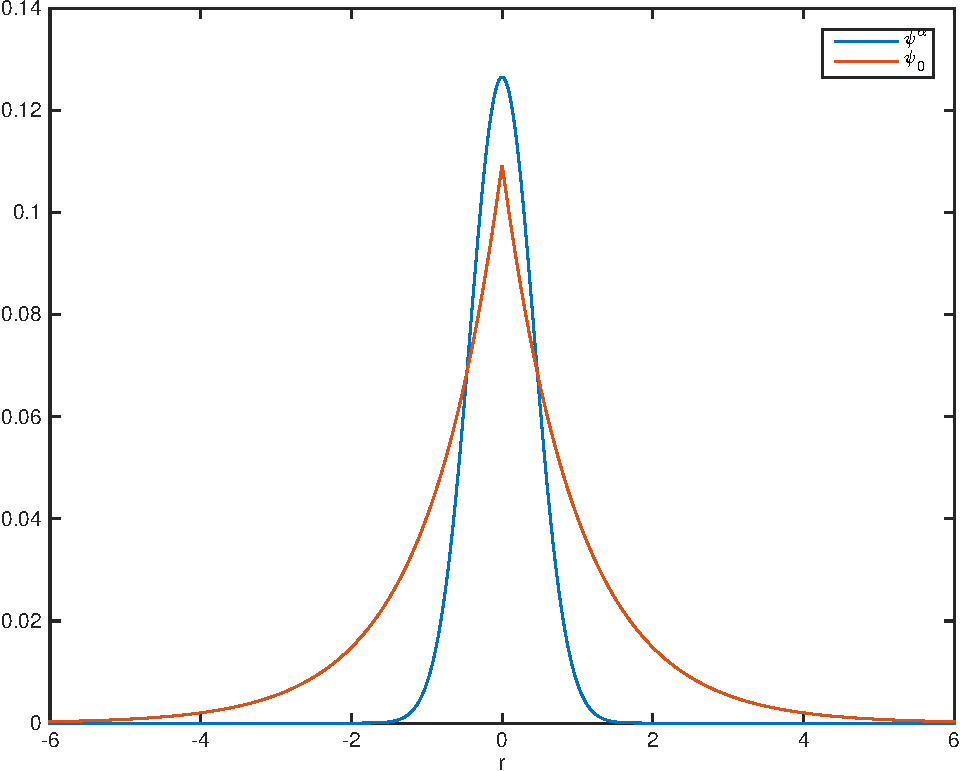
\includegraphics[width=6cm]{hydrogen-gaussian-crop.pdf}
  \end{center}
  \caption{Plot of approximate and exact ground-state wavefunction for
    the Hydrogen example\label{fig:hydrogen}}
\end{figure}

Usually, the set $\mathcal{M}$ contains wavefunction ans\"atze that
are parameterized in some way. In the example, we had a simple
Gaussian wavefunction parameterized by the width. 




\subsection{The Cauchy interlace theorem and linear models}

Suppose that the set $\mathcal{M}$ is a linear space, i.e., a subspace $\mathcal{V}$
of $L^2_N$ defined by a basis set $\ket{\Phi_I}$, $I = 1, 2, \cdots,
D$. Then the variational procedure is equivalent to computing the
smallest eigenvalue of the matrix
\begin{equation}
  \mathsf{H}_{IJ} = \braket{\Phi_I|\hat{H}|\Phi_J}.
\end{equation}
This is so, because for
\begin{equation}
  \ket{\tilde{\Psi}} = \sum_{I=1}^D A_I \ket{\Phi_I}
\end{equation}
the expectation value becomes
\begin{equation}
  \mathcal{E}(\ket{\tilde{\Psi}}) = \frac{ \mathsf{A}^H \mathsf{H}
    \mathsf{A}}{\mathsf{A}^H \mathsf{A}}, \label{eq:matrix-expt}
\end{equation}
which is simply the expectation value functional for the quantum
system with the Hamiltonian $\mathsf{H}$ and wavefunction
$\mathsf{A}$, and we can apply the variational principle to this functional.


It is a fact, that under very mild assumptions on $\{\ket{\Phi_I}\}$
and $\hat{H}$, the eigenvalues of the matrix $\mathsf{H}$ converge
to the eigenvalues of $\hat{H}$, even in the infinite dimensional
case.

For the finite-dimensional case, the Cauchy interlace theorem states
that for a linear model as here described, \emph{all} the eigenvalues
of $\mathsf{H}$ actually approximate eigenvalues of the full
Hamiltonian $\mathsf{H}$ from above. For a general nonlinear model
$\mathcal{M}$, we cannot say this. In general \emph{only} the
ground-state energy is approximated.


The theorem implies that \emph{truncating a
  single-particle basis} or \emph{truncating a Slater determinant
  basis} makes sense.

We will not prove the theorem.

\begin{theorem}[Cauchy Interlace Theorem]
  Let $\mathcal{V}_1$ and $\mathcal{V}_2$ be linear spaces, of
  dimension $D_1$ and $D_2$, respectively. Let $\mathcal{V}_1
  \subset \mathcal{V}_2$ be a subspace.

  Let $\{\ket{\Phi_I}\}_{I=1}^{D_2}$ be an
  orthonormal basis for $\mathcal{V}_2$, such that
  $\{\ket{\Phi_I}\}_{I=1}^{D_1}$ is a basis for $\mathcal{V}_1$.
  
  Let $\hat{H} : \mathcal{V}_2 \to \mathcal{V}_2$ be a Hermitian
  operator with matrix $\mathsf{H}_2 \in \CC^{D_2\times D_2}$,
  $\mathsf{H}_{IJ} = \braket{\Phi_I|\hat{H}|\Phi_J}$.

  Let $\mathsf{H}_1$ be the projection of $\hat{H}$ onto
  $\mathcal{V}_1$, i.e., the matrix $\mathsf{H}_1$ of this operator is
  equal to the upper left $D_1\times D_1$ block of the $D_2\times D_2$ matrix $\mathsf{H}_2$.
  
  Let $E^{(i)}_k$ be the $D_i$ eigenvalues of $\mathsf{H}_i$,
  arranged such that
  \begin{equation}
    E^{(i)}_{k} \leq E^{(i)}_{k+1} \quad \forall k.
  \end{equation}

  Then,
  \begin{equation}
    E_k^{(2)} \leq E_k^{(1)} \leq E_{k+\delta}^{(2)}, \quad \delta =
    D_2 - D_1.
  \end{equation}
\end{theorem}


\begin{exercise}
  Prove Eq.~\eqref{eq:matrix-expt}.
\end{exercise}



\section{The Configuration-interaction method (CI)}
\label{se:ci}

\subsection{General description}


We now describe an approach to manybody theory called
\emph{configuration-interaction theory} (CI). It basically entails
truncating both the single-particle basis and the resulting Slater
determinant basis according to certain rules.

Let an orthonormal single-particle basis $\{\phi_p\}$ be given, with associated
creation operators $c^\dag_p$, and corresponding Slater determinants
$\ket{\vec{p}}$. Suppose we expand an $N$-fermion wavefunction in
the Slater determinant basis, but \emph{truncate} the expansion, including only a finite
subset $\mathcal{S}$ of Slater determinants. The determinants then span a
$D$-dimensional subspace of $L^2_N$,
\begin{equation}
  \mathcal{V} = \operatorname{span} \{ \ket{\vec{p}} \; \big| \; \ket{\vec{p}} \in
  \mathcal{S} \}
\end{equation}
Equivalently, any wavefunction in $V$ can be written
\begin{equation}
  \ket{\Psi} = \sum_{\vec{p}\in\mathcal{S}} A_{\vec{p}} \ket{\vec{p}},
  \quad A_{\vec{p}} = \braket{\vec{p}|\Psi}.
\end{equation}



% Typically, we introduce some indexing scheme $I = I(\vec{\mu})$, $I =
% 1,2,\cdots,D$, so that
% \begin{equation}
%   \ket{\Psi} = \sum_{\vec{\mu} \in \mathcal{S}}
%   \braket{\vec{\mu}|\Psi} \ket{\vec{\mu}} = \sum_{I=1}^D
%   \braket{I|\Psi} \ket{I}.
% \end{equation}
% Exactly one $\ket{I}$ corresponds to one $\ket{\vec{\mu}}$.

The set $\mathcal{S}$ may of course be chosen in many different
ways. One typical choice is the set of all possible Slater
determinants generated by the first $L$ single-particle functions
$\phi_0$ through $\phi_{L-1}$. This gives a space of dimension
$\binom{L}{N}$, and is called the \emph{full configuration-interaction
  space} (FCI space).

Another typical approach is to have a \emph{reference determinant}
$\ket{\Phi}$ and consider particle-hole states on top of that, or
excitations in chemistry language.

For example, the one-particle-one-hole space (CI singles, CIS)
wavefunction is given by the choice
\begin{equation}
  \mathcal{V}_\text{CIS} = \operatorname{span} \{ \ket{\Phi}, \; \ket{\Phi_i^a} \; \big| \;
  i = 1,\cdots N, \; a = N+1,\cdots, L \},
\end{equation}
and any CIS wavefunction can thus be written
\begin{equation}
  \ket{\Psi} = A_0 \ket{\Phi} + \sum_{ia} A_{i}^{a} \ket{\Phi_{ia}}.
\end{equation}
Furthermore, CI singles-and-doubles (CISD) is defined by the space
\begin{equation}
  \mathcal{V}_\text{CISD} = \operatorname{span} \{ \ket{\Phi}, \; \ket{\Phi_i^a}
  \; \ket{\Phi_{ij}^{ab}} \big| \;
  i,j = 1,\cdots N, \; a,b = N+1,\cdots, L \}.
\end{equation}
A wavefunction $\ket{\Psi} \in V_\text{CISD}$ can be written
\begin{equation}
  \ket{\Psi} = A_0 \ket{\Phi} + \sum_{ia} A_{i}^{a} \ket{\Phi_{i}^a} +
   \sum_{i<j}\sum_{a<b} A_{ij}^{ab} \ket{\Phi_{ij}^{ab}}.
\end{equation}
Configuration-interaction singles-doubles-and-triples (CISDT), etc,
are defined similarly. 

Sometimes, the doubles term is written
\begin{equation}
  \sum_{i<j}\sum_{a<b} A_{ij}^{ab} \ket{\Phi_{ij}^{ab}} = \frac{1}{4}
  \sum_{ij}\sum_{ab} A_{ij}^{ab} \ket{\Phi_{ij}^{ab}}.
\end{equation}
The coefficients satisfy $A_{ij}^{ab} = -A_{ji}^{ab} = - A_{ij}^{ba} =
A_{ji}^{ba}$, and the factor $1/4$ comes from the fact that
$\ket{\Phi_{ij}^{ab}} = - \ket{\Phi_{ij}^{ba}} = -
\ket{\Phi_{ji}^{ab}} = \ket{\Phi_{ji}^{ba}}$, i.e., we are deliberately
  over-counting the basis in this expression to keep notation simple.

\begin{exercise}
  Compute the dimension of $\mathcal{V}_\text{CIS}$, $\mathcal{V}_{\text{CISD}}$, etc.
\end{exercise}

Clearly, indexing the Slater determinants using the
vector $\vec{p}$ directly can be cumbersome. Using a different notation,
we let $I \in \mathcal{I}$ be an index that enumerates the basis
determinants, and write
\begin{equation}
  \mathcal{V} = \operatorname{span} \{ \ket{\Phi_I} \; \big| \; I \in
  \mathcal{I} \}.
\end{equation}
Our vector
expansion becomes
\begin{equation}
  \ket{\Psi} = \sum_{I} A_{I} \ket{\Phi_I},
  \quad A_{I} = \braket{\Phi_I|\Psi}.
\end{equation}
For example, $\mathcal{I} = 1,2,\cdots,D$ is a possibility, with some
way of choosing an $I$ for every $\vec{p}$ we are interested in. Or $I
= (a,i)$, $I = (ab,ij)$, etc, enumerates the CIS, CISD, etc, hierarchy
of spaces. 



How do we choose the single-particle functions and the reference state
in CI theory? The most common choice in chemistry is to employ a basis
of \emph{Hartree--Fock spin-orbitals}. This is the topic of
Section~\ref{sec:hf}. A more general picture is as follows: if $\hat{H} = \hat{H}_0 + \hat{W}$, it
is also possible to consider $\hat{W}$ a perturbation of $\hat{H}_0$,
assuming that the eigenstates and eigenvalues of $\hat{H}_0$ are good
approximations to those of the full $\hat{H}$. (This is also true for
the Hartree--Fock paradigm to be considered later.)

Let therefore $\{\phi_p\}$ be a complete set of eigenfunctions for
the single-particle operator $\hat{h}$ with eigenvalues $\epsilon_p$
arranged in increasing order. Then, the Slater determinants
$\ket{\vec{p}}$ are eigenstates of the one-body Hamiltonian
$\hat{H}_0 = \sum_i^N \hat{h}(i)$. Clearly, the determinant
\begin{equation}
  \ket{\Phi} = \ket{123\cdots N}
\end{equation}
is the ground-state wavefunction of $\hat{H}_0$, whose second
quantized expression is
\begin{equation}
  \hat{H}_0 = \sum_p \epsilon_p c^\dag_p c_p.
\end{equation}
Note, that if the
eigenvalues of $\hat{h}$ are degenerate, then this wavefunction may or
may not be unique.

In this picture, the truncated CI scheme as outlined above is a
natural approach, since it is reasonable to assume that singles,
doubles, etc, will systematically improve upon the ``zero-order''
wavefunction $\ket{\Phi}$.

In the context of a reference function $\ket{\Phi}$ defined in terms
of a zero-order Hamiltonian, such as $\hat{H}_0$, it is common to
define the \emph{fermi level} $\epsilon$ as the energy of the occupied
orbital with the highest energy, $\epsilon_\text{F}$, assuming
that all degenerate levels are included. With this terminology,
\begin{equation}
  \ket{\Phi} = \left(\prod_{\epsilon_p \leq \epsilon_\text{F}} c^\dag_p\right) \ket{-},
\end{equation}
for example. Moreover, we say that a \emph{hole} is ``below the Fermi
level'' and a \emph{particle} is ``above the Fermi level''. An
excitation excites a fermion from below the Fermi level to above the
Fermi level. Thus, the index $N$ is replaced by the one-body
\emph{energy} of that level, $\epsilon_{\text{F}}$. See Fig.~\ref{fig:fermi}


Notice that the truncated CI scheme favors the description of the
ground-state wavefunction.

\begin{figure}
  \begin{center}
    \begin{tikzpicture}
      \begin{scope}
        \draw[thick] (0,0)  -- (2,0);
        \draw[thick] (0,.5)-- (2,.5);
        \draw[thick] (0,1) -- (2,1);
        \filldraw (1,1.4) circle (.01cm);
        \filldraw (1,1.5) circle (.01cm);
        \filldraw (1,1.6) circle (.01cm);
        \draw[thick] (0,2) -- (2,2);
        \draw[dashed] (-.5,2.25) node[anchor=east]{$\epsilon_F$} --
        (2.5,2.25);
        
        \draw[thick] (0,2.5)  -- (2,2.5);
        \draw[thick] (0,3)  -- (2,3);
        \draw[thick] (0,3.5) -- (2,3.5);
        \draw[thick] (0,4) -- (2,4);
        
        \filldraw (1,4.4) circle (.01cm);
        \filldraw (1,4.5) circle (.01cm);
        \filldraw (1,4.6) circle (.01cm);
        
        \filldraw (1,0) circle (0.1);
        \filldraw (1,.5) circle (0.1);
        \filldraw (1,1) circle (0.1);
        \filldraw (1,2) circle (0.1);
        
        \draw [decorate,decoration={brace,amplitude=10pt},xshift=-4pt,yshift=0pt]
        (0,2.5) -- (0,5) node [midway,anchor=east,xshift=-10pt] {particles are here};
        
        \draw [decorate,decoration={brace,amplitude=10pt},xshift=-4pt,yshift=0pt]
        (0,0) -- (0,2) node [midway,anchor=east,xshift=-10pt] {holes are here};
      
        \node at(1,-1) {Reference state $\ket{\Phi}$};
      \end{scope}

      \begin{scope}[xshift=4cm]
        \draw[thick] (0,0)  -- (2,0);
        \draw[thick] (0,.5)-- (2,.5);
        \draw[thick] (0,1) -- (2,1);
        \filldraw (1,1.4) circle (.01cm);
        \filldraw (1,1.5) circle (.01cm);
        \filldraw (1,1.6) circle (.01cm);
        \draw[thick] (0,2) -- (2,2);
        \draw[dashed] (-.5,2.25) node[anchor=east]{$\epsilon_F$} --
        (2.5,2.25);
        
        \draw[thick] (0,2.5)  -- (2,2.5);
        \draw[thick] (0,3)  -- (2,3);
        \draw[thick] (0,3.5) -- (2,3.5);
        \draw[thick] (0,4) -- (2,4);
        
        \filldraw (1,4.4) circle (.01cm);
        \filldraw (1,4.5) circle (.01cm);
        \filldraw (1,4.6) circle (.01cm);
        
        \filldraw (1,0) circle (0.1);
        \draw (1,.5) circle (0.1);
        \filldraw (1,1) circle (0.1);
        \draw (1,2) circle (0.1);
      
        \filldraw (1,3) circle (0.1);
        \filldraw (1,4) circle (0.1);

        \node at(1,-1) {$\ket{\Phi_{ij}^{ab}}$};
      \end{scope}
      
    \end{tikzpicture}
  \end{center}
  \caption{Fermi level and quasiparticles\label{fig:fermi}. To the
    left, we have the vacuum state. To the right, we have a doubly
    excited state, or a two-particle-two-hole-state. Notice how we
    draw the ``Fermi line'' between two levels for clarity. In this
    simple picture, we have assumed that the levels are
    non-degenerate. If we had spin present, we could fit two particles
    per level, and so on.}
\end{figure}


\subsection{Matrix elements of the CI method}
\label{sec:ci-mat-elem}




Having established the parametrization of the approximate
wavefunction, a linear space $\mathcal{V}$, we turn to the variational principle,
which tells us (together with the Cauchy Interlace Theorem that) that
the matrix of the Hamiltonian $\hat{H}$ with respect to the chosen
basis is the central object. Diagonalizing this matrix gives us
approximations to the ground-state energy and in total $D$ eigenvalues
of the full system.

Thus, in the CI method, we need to diagonalize the matrix $H = [H_{IJ}]$
given by
\begin{equation}
  H_{IJ} = \braket{\Phi_I|\hat{H}|\Phi_J}
\end{equation}
%
%Here, the index $I$ counts the reference state ($I=0$), the singles
%($I=1,\cdots, N\times (L-N)$), the doubles, and so on. Thus, the particle-hole indices
%are converted to an ordinary integer.

If we look at the CISD case, the matrix then obtains a block form:
\begin{equation}
  \mathsf{H} = \left(\begin{array}{c|c|c} 
      \braket{\Phi|\hat{H}|\Phi} &
    \braket{\Phi|\hat{H}|\Phi_i^a} &
    \braket{\Phi|\hat{H}|\Phi_{ij}^{ab}} \\ \hline
    \braket{\Phi_{i'}^{a'}|\hat{H}|\Phi} &
    \braket{\Phi_{i'}^{a'}|\hat{H}|\Phi_{i}^a} &
    \braket{\Phi_{i'}^{a'}|\hat{H}|\Phi_{ij}^{ab}} \\ \hline 
    \braket{\Phi_{i'j'}^{a'b'}|\hat{H}|\Phi} &
    \braket{\Phi_{i'j'}^{a'b'}|\hat{H}|\Phi_{i}^a} &
    \braket{\Phi_{i'j'}^{a'b'}|\hat{H}|\Phi_{ij}^{ab}}
  \end{array}\right)
\end{equation}

% The Hamiltonian in second-quantized form is
% \begin{equation}
%   \hat{H} = \sum_p h^p_q c^\dag_p c_p +
%   \frac{1}{4}\sum_{pqrs} w^{pq}_{sr} c^\dag_p  c^\dag_q c_s c_r.
% \end{equation}
% In the previous section, we assumed that $\hat{h}\ket{\phi_p} =
% \epsilon_p \ket{\phi_p}$, which makes the matrix
% $h^p_q$ diagonal. This is not necessary, however,
% and we will not assume this in the present section. We \emph{do
%   assume} however, that $w^{pq}_{sr}$ is anti-symmstrized, at odds
% with the initial definition of these sybols, for brevity.

% In general, the matrix elements $h^p_q$ and $w^{pq}_{rs}$ need to
% be computed from the given single-particle basis
% $\{\phi_p\}$. This is a task on its own. Assuming that this has been
% done, we consider the task of computingt he matrix elements.

% There are several options: One can use the Slater--Condon rules, see
% Exercise~\ref{exercise:slater-condon-rules}, which basically give
% formulae for the matrix elements in terms of the single-particle
% functions $\vec{p}_I$ and $\vec{P}_{J}$ of $\ket{\Phi_I}$ and
% $\ket{\Phi_J}$. The important 


% let us evaluate the blocks of $\mathsf{H}$. Here, the
% normal-ordered Hamiltonian comes in handy,
% \begin{equation}
%   \hat{H} = E_0 + \hat{H}_\text{N} = E_0 + \hat{H}_{0,\text{N}} + \hat{W}_\text{N}.
% \end{equation}
% Consider first
% \begin{equation}
%   \braket{\Phi|\hat{H}|\Phi} = E_0 + \braket{\Phi|\hat{H}_N|\Phi} =
%   E_0,
% \end{equation}
% where the term with $\hat{H}_N$ vanishes since it is normal ordered
% with at least one (two) operators, and hence has a zero vacuum expectation value.
% Consider next
% \begin{equation}
%   \braket{\Phi|\hat{H}|\Phi_i^a} =
%   \braket{\Phi|(\hat{H}_{0,\text{N}} + \hat{W}_\text{N})|\Phi_i^a}.
% \end{equation}
% Consider the one-quasiparticle term:
% \begin{equation}
%   \braket{\Phi|\hat{H}_{0,\text{N}}|\Phi_i^a} = \sum_{pq} (h^p_q +
%   \sum_k w^{pk}_{qk})
%   \braket{\Phi|N(c^\dag_p c_q) b^\dag_a b^\dag_i |\Phi}.
% \end{equation}
% We can only have a contribution if $N(c^\dag_p c_q)$ represents a
% two-quasiparticle annihilation, i.e., $pq=ja$ are the only
% contributing terms:
% \begin{equation}
%   \braket{\Phi|\hat{H}_{0,\text{N}}|\Phi_i^a} = \sum_{jb} (h^j_b +
%   \sum_k w^{jk}_{bk})
%   \braket{\Phi|b_j b_b b^\dag_a b^\dag_i |\Phi} = h^i_a + \sum_k w^{ik}_{ak}.
% \end{equation}

% The rest of the matrix elements can easily be computed in a similar
% fashion, using Wick's theorem applied to vacuum expectation values for
% quasiparticle operators.

% We here only list the matrix elements, and leave their evaluation as
% an exercise.

% \note{Update with matrix elements and exercises.}

\subsection{Computer implementation of CI methods}

In chemistry, \emph{speed} and \emph{reliability} are crucial
factors. Computations are performed by non-specialists using highly
optimized codes like \programname{Dalton}, \programname{Molpro}, or
\programname{Gaussian}.

We will not try and compete with such codes, of course, but instead
indicate how various methods may be implemented.

\subsection{Naive CI}

The simplest approach, which we here call ``naive CI'', is to
\begin{enumerate}
\item
  Write down a list of all the Slater determinants in the desired
  basis,
  \[ I \mapsto \ket{\Phi_I}. \]
\item
  Compute all the matrix elements $H_{IJ}$ and store them in computer
  memory as a big $D\times D$ matrix. This can be done using, say, the
  Slater--Condon rules (see
  Exercise~\ref{exercise:slater-condon--rules}) that are basically
  formulae for the matrix elements given in terms of the occupied
  single-particle functions in $\ket{\Phi_I}$ and $\ket{\Phi_J}$.
\item
  Use a diagonalization agorithm to find, say, the ground-state energy
  or other eigenvalues of the matrix.
\end{enumerate}

The biggest problem with this approach, is that the dimension $D$ of
the CI space grows pretty fast. The matrix is, in principle, a table
with $D^2$ elements. For FCI, $D$ grows like $\binom{L}{N}$, which
very quickly is prohibitive. For CIS, it grows only like $N(L-N)$, but
CIS is not that fancy. For CISD, the dimension grows like $N^2
(L-N)^2$. We see that the spaces in any case become huge for moderate
partucle numbers and numbers $L$ of single-particle functions.

\subsection{Direct CI}

More common than ``naive CI'' is direct CI. For systems of interest,
the matrix size grows so quickly that storing the matrix $H$ in memory
is out of question. Moreover, diagonalization of dense matrices scales
as $D^3$, quickly becoming too expensive for practical calculations.

Luckily, we have \emph{iterative algorithms} such as the Lanczos
algorithm. These rely only on the \emph{matrix-vector product}. Nowhere
is the actual value of $H_{IJ}$ needed, only the action on a vector
$A_I$, i.e., the algorithm needs to compute
\begin{equation}
  \vec{A}'  = H\vec{A}
\end{equation}
for some input vector $\vec{A}$. I.e., we must have an algorithm to
compute 
\begin{equation}
  \ket{\Psi'} = P \hat{H}\ket{\Psi}
\end{equation}
where $P = \sum_I \ket{\Phi_I}\bra{\Phi_I}$ is the projection operator
onto our chosen basis, i.e., we throw away the part of
$\hat{H}\ket{\Psi}$ which is not describable in terms of our basis.

It is useful to represent $\ket{\Phi_I}$ in terms of its occupation
number vector, a bit string $B = B[I]$. These are integers, and we
need a table of these in computer memory. Since our $\ket{\Phi_I}$
must be linearly independent, there is a one-to-one correspondence
between the $B[I]$'s and the $I$'s, i.e., we can \emph{invert} the
table to obtain $I = I[B]$, given $B$. We write $\ket{B} =
\ket{\Phi_{I[B]}}$ for brevity, and we stress that now $B$ is an
integer written on binary form.

The central observation is now that, for any string of creation and
annihilation operators
\begin{equation}
  C_1 C_2 \cdots C_n \ket{B} = \begin{cases} 0 & or \\ (-1)^s
    \ket{B'} \end{cases}.
\end{equation}
The result can be found by \emph{manipulating the bits of $B$ and
  keeping track of the resulting sign.} When $B'$ has been found, the
corresponding index $I'$ can be found by searching the bit pattern
table. Thus, let us write:
\begin{equation}
  \begin{split}
    \ket{\Psi'} &= P \hat{H}\ket{\Psi} = \sum_{B'}
    \ket{B'}\bra{B'} \hat{H} \sum_B A_B \ket{B} \\
    & = \sum_B A_B \sum_{B'} \ket{B'} \bra{B'}\left(\sum_{pq} h^p_q
      c^\dag_p c_q + \tfrac{1}{4}\sum_{pqrs} w^{pq}_{rs} c^\dag_p
      c^\dag_q c_s c_r \right) \ket{B} \\
 & =
  \ket{\Psi'} = \sum_B A_B \left(\sum_{pq} h^{p}_q \braket{B'|c^\dag_p c_q|B} +
  \tfrac{1}{4}\sum_{pqrs} w^{pq}_{rs} \braket{B'|c^\dag_p c^\dag_q c_s
    c_r|B}\right) \ket{B'}
\end{split}
\end{equation}
This gives us the following algorithm for computing the $\hat{H}_0$
contribution to $\ket{\Psi'}$ (the $\hat{W}$ part is similar):
\begin{enumerate}
\item
  Initialize $A'_{I'} = 0$ for all $I'$.
\item
  Loop over $I$:
  \begin{enumerate}
  \item
    Fetch $B = B[I]$.
  \item
    Loop over $p,q$.
    \begin{enumerate}
    \item
      Compute $c^\dag_p c_q \ket{B} = 0$ or $(-1)^s\ket{B'}$ by
      manipulaing the bits in $B$.
    \item
      If the result is nonzero, compute $I'$ such that $B[I'] = B'$ by
      searching the bit pattern table.
    \item
      If the pattern is found, update $A'_{I'} \leftarrow A'_{I'} +
      A_I h^{p}_q (-1)^s$.
      
    \end{enumerate}
  \end{enumerate}  
\end{enumerate}

Of course, this algorithm is just a sketch. There are many ways to
improve it.

How does one search for the index $I'$ in step 2/b/ii? One way is to
ensure that the table of bit patterns (integers) are sorted, and then
use \emph{binary search}. This requires on average $O(D \log D)$
operations, and since we need to do this $O(D)$ times, this slows down
our program drastically. One can also use a \emph{hash map} (e.g., the
C++ STL class \texttt{std::map<int,int>} can be used). This is no
faster.

A \emph{much} faster approach can be taken using \emph{graphical
  methods}. It is actually possible to find a formula for the inverse
map. This formula is $O(1)$, dramatically reducing the computer work
for direct CI. For more information on this technique, see
Helgaker/J{\o}rgensen/Olsen \cite{HJO}, Section 11.8. 


\subsection{Recipe for bit pattern representation.}

How can we perform the bitwise operations mentioned above?

Each Slater determinant $\ket{\mu_1,\cdots\,\mu_N}$ is, via the
occupation numbers, mapps to the bit pattern $\ket{n_0 n_1 n_2\cdots n_L}$ where each
$n_\mu \in \{0,1\}$. We identify the bit pattern with the integer
$B[\mu_\cdots \mu_N]$ it encodes. Thus,
\begin{equation}
  \vec{\mu} = \{1, 5, 6\} \mapsto \ket{\underbrace{010001100\cdots
      0_2}_{\text{$L$ bits}}} \mapsto \ket{ 1\times 2^1 + 1\times 2^5 +
    1\times 2^6} = \ket{ 97_{10}}.
\end{equation}
(But who is thinking in terms of base-10 numbers these days anyway?)
All integers between 0 and $2^{L-1}$ encode all possible Fock space
basis functions. A basis for $N$-fermion space is composed of all the
integers whose bit patterns have precisely $N$ bits in total.

Annihilation operator: $c_p \ket{B}$ is either $0$ or
$(-1)^k\ket{B'}$ for some $k$ and $B'$. We have the
following algorithm:
\begin{enumerate}
\item
  If bit $p$ is not set, return the zero result.
\item
  Else, compute $k$ as the number of bits set \emph{before} $p$.
\item
  Erase bit $p$  to obtain $B'$.
\item
  Retun the sign $(-1)^k$ and $B'$.
\end{enumerate}

Creation operator:
$c^\dag_p \ket{B}$ is either $0$ or
$(-1)^k\ket{B'}$ for some $k$ and $B'$. We have the
following algorithm:
\begin{enumerate}
\item
  If bit $p$ is set, return the zero result.
\item
  Else, compute $k$ as the number of bits set \emph{before} $p$.
\item
  Light bit $p$ to obtain $B'$.
\item
  Return the sign $(-1)^k$ and $B'$.
\end{enumerate}


The product $c^\dag_p c_q \ket{B}$ can be computed by repeating the
above algorithms, and similarly with $\emph{any}$ string of creation
and annihilation operators.


\begin{exercise}
  We are given $L=8$ orbitals, numbered $p=0,1,\cdots,L-1$, and thus
  an occupation number representation of length $8$ bits, e.g.,
  \begin{equation}
    \ket{p=2,p=3} = \ket{0_0 0_1 1_2 1_3 0_4 0_5 0_6 0_7 } =
    \ket{00110000}.
  \end{equation}
  Write down the result of the following expressions, on occupation
  number form. Remember the sign factor:
  \begin{enumerate}
  \item[a)] $c^\dag_1         \ket{01100000}$
  \item[b)] $c_5             \ket{01000101}$
  \item[c)] $c^\dag_4 c^\dag_1 \ket{01101000}$
  \item[d)] $c^\dag_1         \ket{01100000}$
  \item[e)] $c_6             \ket{11111111}$
  \item[f)] $c^\dag_6         \ket{01111001}$
  \item[g)] $c^\dag_1 c^\dag_2 c^\dag_3  \ket{00000000}$
  \item[h)] $c^\dag_4c_4      \ket{11101000}$
  \end{enumerate}      
\end{exercise}


\begin{exercise}\label{ex:ci1}
  Write a program that generates all possible bit patterns of length
  $L$ with $N$ bits set and writes them to screen.

  Check that you have the correct number of patterns, $\binom{L}{N}$.
\end{exercise}

\begin{exercise}\label{ex:ci2} (continues exercise~\ref{ex:ci1}.)
  Write a program that correctly creates/annihilates particles from a
  bit pattern representation $\ket{B}$ of a Slater determinant,
  returning the proper sign.
\end{exercise}

\begin{exercise}\label{ex:ci3} (continues exercises~\ref{ex:ci1} and \ref{ex:ci2}.)
  Write a program that, given $h^{p}_q$ and $w^{pq}_{rs}$
  (antisymmetrized or otherwise) as input
  arrays, computes $\hat{H}\ket{B}$ using direct CI.
\end{exercise}



\section{Hartree--Fock theory (HF)}
\label{sec:hf}

\subsection{The Hartree--Fock equations}
\label{sef:hf-equations}


Suggested reading for this section: Szabo/Ostlund Ch.~13,
Harris/Monkhorst/Freeman Ch.~3, Gross/Runge/Heinonen Ch.~7.

It is highly recommended to read the mathematical supplement in the
Appendix, Sec.~\ref{sec:calculus-of-variations} on the calculus of
variations.

One of the earliest and most successful approximation methods for
many-fermion systems was the \emph{Hartree--Fock method} (HF method). In
Hartree--Fock theory we parametrize our wavefunction as a single Slater
determinant. However, \emph{the single-particle functions are the
  unknowns to be determined by the variational procedure}.

Thus, our wavefunction manifold $\mathcal{M}$ consists of all possible
functions on the form
\begin{equation}
  \ket{\Phi} = \ket{\phi_1 \phi_2 \cdots \phi_N}, \quad
  \braket{\phi_i|\phi_j}= \delta_{ij}.
\end{equation}
Note carefully, that a single-particle basis is not given -- it is to
be found!
%
%We have
%\begin{equation}
%  \mathcal{E}(\ket{\Phi}) = \braket{\Phi|\hat{H}|\Phi} = \sum_i
%  \braket{\phi_i|\hat{h}|\phi_i} + \frac{1}{2}\sum_{ij} \braket{\phi_i
%    \phi_j | \hat{w} |\phi_i\phi_j - \phi_j\phi_i}, 
%\end{equation}
%as established in the CI theory. 
The expectation value of the Hamiltonian $\hat{H} = \hat{H}_0 +
\hat{W}$ now reads (recalling
that $\braket{\Phi|\Phi}=1$)
\begin{equation}
  \braket{\Phi|\hat{H}|\Phi} = \sum_i 
  \braket{\phi_i|\hat{h}|\phi_i} + \frac{1}{2}\sum_{ij} \braket{\phi_i
    \phi_j | \hat{w} |\phi_i\phi_j - \phi_j\phi_i}
  \label{eq:hf-energy}
\end{equation}
as obtained via the Slater--Condon rules, see for example
Exercise~\ref{exercise:slater-condon-rules}. Here,
\begin{equation}
  \braket{\phi_p\phi_q|\hat{w}|\phi_r\phi_s} \equiv \int
  dx_1\int dx_2 \phi_p(x_1)^*\phi_q(x_2)^* w(x_1,x_2)
  \phi_r(x_1)\phi_s(x_2),
\end{equation}
which satisfies
$\braket{\phi_p\phi_q|\hat{w}|\phi_r\phi_s}=\braket{\phi_q\phi_p|\hat{w}|\phi_s\phi_r}$. 
The task is now to minimize this energy $\braket{\Phi|\hat{H}|\Phi}$
subject to the constraint that the $\phi_i$ are orthonormalized,
\begin{equation}
  \braket{\phi_i|\phi_j} = \delta_{ij}.
\end{equation}
When a minimum is found, we denote the solution by
$\ket{\Phi_\text{HF}}$, the Hartree--Fock state.

The constraints constitute a complication that we want to get rid
of. We therefore \emph{Lagrange multipliers}, one for each constraint, giving
a Lagrangian functional
\begin{equation}
  \begin{split}
  \mathcal{L}[\phi_1,\cdots,\phi_N, \lambda] &=
  \braket{\Phi|\hat{H}|\Phi} -
  \sum_{ij}\lambda_{ji}(\braket{\phi_i|\phi_j} - \delta_{ij}) \\
  &=\sum_i 
  \braket{\phi_i|\hat{h}|\phi_i} + \frac{1}{2}\sum_{ij} \braket{\phi_i
    \phi_j | \hat{w} |\phi_i\phi_j - \phi_j\phi_i} -
  \sum_{ij}\lambda_{ji}(\braket{\phi_i|\phi_j}-\delta_{ij}) \label{eq:hf-lagrangian}
\end{split}
\end{equation}
Recall, that computing an extremum for the constrained
problem is equivalent to an \emph{unconstrained} extremalization of
$\mathcal{L}$ with respect to the $\phi_i$ \emph{and} the Lagrange
multipliers (see any text on vector calculus). 

Due to symmetry of the constraints, the Lagrange multiplier matrix
$\lambda$ can be assumed to be Hermitian\footnote{To see this, assume
  that $a_{ji}$ is a matrix which is not assumed to be Hermitian. Note
  that the expression $g_{ij} = \braket{\phi_i|\phi_j}-\delta_{ij}$
  satisfies $g_{ij}^* = g_{ji}$. Thus, $\sum_{ij} a_{ji} g_{ij} =
  \sum_{ij} a_{ji} g_{ji}^* = \sum_{ij} a_{ij} g_{ij}^* = (\sum_{ij}
  a_{ij}^* g_{ij})^*$. This gives $\sum_{ij} a_{ji}g_{ij} =
  \tfrac{1}{2}\sum_{ij}(a_{ji}+a_{ij}^*)g_{ij}$. Take $\lambda_{ji}=
  a_{ji}+a_{ij}^*$.}. 


A word on a special notation. We define a single-particle function
\begin{equation}
  \braket{\;\cdot\; \phi_1|\hat{w}|\phi_2\phi_3} \in L^2_1
\end{equation}
as the function obtained by integrating only over the
second particle in the inner product, viz,
\begin{equation}
  \bra{x_1}\braket{\;\cdot\; \phi_1|\hat{w}|\phi_3 \phi_3} = \braket{\;\cdot\; \phi_1|\hat{w}|\phi_3 \phi_3}(x_1) \equiv \int
  \phi_1(x_2)^* [w(x_1,x_2) \phi_2(x_1)\phi_3(x_2)] \; dx_2.
\end{equation}
The inner product with any single-particle function $\chi$ is
\begin{equation}
  \bra{\chi}\braket{\;\cdot\; \phi_1|\hat{w}|\phi_2 \phi_3} = \iint
  \chi(x_1)^* \phi_1(x_2)^* [w(x_1,x_2) \phi_2(x_1)\phi_3(x_2)] \; dx_1
  dx_2 = \braket{\chi\phi_1|\hat{w}|\phi_2\phi_3},
\end{equation}
i.e., the full two-particle integral. Thus, the dot represents an
``unused slot'' in the two-particle matrix element. 

We can expand the
function in any orthonormal single-particle basis $\{\chi_p\} \subset
L^2_1$,
\begin{equation}
  \braket{\;\cdot\; \phi_1|\hat{w}|\phi_2\phi_3} = \sum_p
  \ket{\chi_p}\bra{\chi_p}\braket{\;\cdot\; \phi_1|\hat{w}|\phi_2\phi_3}
    = \sum_p
  \ket{\chi_p}\braket{\chi_p \phi_1|\hat{w}|\phi_2\phi_3}, \label{eq:emptyslot}
\end{equation}
i.e., a linear combination of to-particle matrix elements.
This notation will be useful when we now state and prove our result:
\begin{theorem}[Hartree--Fock equations]\label{thm:hf-equations}
  The single-particle functions of the Hartree--Fock state
  $\ket{\Phi_\text{HF}}$ satisfy
%Suppose the single-particle functions $\phi_i$, $i=1,\cdots N$ satisfy
  the nonlinear eigenvalue problem
  \begin{equation}
    \hat{f}(\phi_1,\cdots,\phi_N)\ket{\phi_i} = \epsilon_i
    \ket{\phi_i}, \label{eq:hf-can}
  \end{equation}
  where
  \begin{equation}
    \hat{f}(\phi_1,\cdots,\phi_N) \equiv \hat{h} + \hat{v}^\text{direct}
     - \hat{v}^\text{exchange},\label{eq:fock-op}
  \end{equation}
  with
  \begin{equation}
    \hat{v}^\text{direct}\ket{\psi} \equiv \sum_j \braket{\; \cdot \;
      \phi_j|\hat{w}|\psi\phi_j}. \label{eq:direct}
  \end{equation}
  and
  \begin{equation}
    \hat{v}^\text{exchange}\ket{\psi} \equiv \sum_j \braket{\; \cdot \;
      \phi_j|\hat{w}|\phi_j\psi}. \label{eq:exchange}
  \end{equation}
  % \begin{equation}
  %   \bra{x}\hat{v}^\text{direct}\ket{\psi} = \int dy \sum_{j=1}^N
  %   |\phi_j(y)|^2 w(x,y)
  % \end{equation}
  % being a local potential, while
  % \begin{equation}
  %   \bra{x}\hat{v}^\text{exchange}\ket{\psi} = \int dy \sum_{j=1}^N
  %   \phi_j(y)^* \psi(x)  w(x,y) \phi_j(x)
  % \end{equation}
  % is non-local. 

 % Then, $\ket{\phi_1\cdots\phi_N}$ is a stationary point of
 % $\mathcal{E}$ under all possible variations of the $\phi_i$ that
 % preserve orthonormality. 
  The equations~\eqref{eq:hf-can} are
  referred to as ``the Hartree--Fock equations''. The operator
  $\hat{f}$ in Eq.~\eqref{eq:fock-op} is ``the Fock operator'', and
  $\hat{v}^\text{direct}$ and $\hat{v}^\text{exchange}$ are the direct-
  and exchange potentials, respectively.
\end{theorem}

\begin{proof}
  In the language of Sec.~\ref{sec:calculus-of-variations}, we need to
  show that the directional derivative of the Lagrangian
  vanishes.

  We first note that $\lambda_{ji}$ can be treated separately:
  $\partial \mathcal{L}/\partial \lambda_{ji} = \braket{\phi_i|\phi_j}
  - \delta_{ij}$, the constraint. These equations are ensured
  fulfilled in the end by finding solutions $\phi_i$ that are in fact
  orthonormal. We thus only compute the directional derivatives with
  respect to variations of the $\phi_i$.

  %As in the proof for the variational principle, we can treat $\phi_i$
  %and $\phi_i^*$ as independent variables, varying only the bra
  %states (see Exercise \ref{exercise:vp-complex}). 

  Choose a $k\in\{1,\cdots,N\}$.
  We are going to compute the directional derivative with respect to
  changes in the function $\phi_k$ only, leaving the other
  fixed. This turns out to be sufficient to find all the equations. Thus,
  let $\epsilon$ be a small real number, and let ${\eta}$ be a
  normalized single-particle function. We write
  \[ {\delta\phi_k} = \epsilon \eta. \]
  The other functions are fixed, $\delta \phi_i = 0$ for $i\neq k$.
  Define the function
  \begin{equation}
    f(\epsilon) = \mathcal{L}(\phi_1,\cdots,\phi_k +
    \epsilon\eta,\cdots,\phi_N, \lambda), 
  \end{equation}
  To first order in $\epsilon$,
  \begin{equation}
    f(\epsilon) = f(0) + \epsilon f'(0) + O(\epsilon^2),
  \end{equation}
  and we for an extremal point of $\mathcal{L}$, we must have that for
  any $\eta$, $f'(0)=0$.
  In the language of
  Sec.~\ref{sec:calculus-of-variations}, the directional derivative of
  $\mathcal{L}$ at $\{\phi_i\}_{i=1}^N$ in the direction
  $\eta$ (for $\phi_k$, the others are fixed) vanishes. 

  We compute the Taylor expansion of $f(\epsilon)$ by direct
  computation of the perturbed Lagrangian:
  \begin{equation}
    \begin{split}
      f(\epsilon) 
      %&= \mathcal{L}(\phi+\delta\phi,\lambda) = \sum_i
      %\braket{\phi_i + \delta\phi_i|\hat{h}|\phi_i + \delta\phi_i} +
      %\frac{1}{2}\sum_{ij} \braket{(\phi_i + \delta\phi_i)(\phi_j +
      %  \delta\phi_j)|\hat{w}|(\phi_i + \delta\phi_i)(\phi_j +
      %  \delta\phi_j)} \\ &\qquad - \frac{1}{2}\sum_{ij}
      %\braket{(\phi_i + \delta\phi_i)(\phi_j +
      %  \delta\phi_j)|\hat{w}|(\phi_j + \delta\phi_j)(\phi_i +
      %  \delta\phi_i)} - \sum_{ij} \lambda_{ij}(\braket{\phi_i +
      %  \delta\phi_i|\phi_j + \delta\phi_j} - \delta_{ij}) \\
      &= \sum_i
      \braket{\phi_i + \delta_{ki}\epsilon\eta|\hat{h}|\phi_i + \delta_{ki}\epsilon\eta} +
      \frac{1}{2}\sum_{ij} \braket{(\phi_i + \delta_{ki}\epsilon\eta)(\phi_j +
        \delta_{kj}\epsilon\eta)|\hat{w}|(\phi_i + \delta_{ki}\epsilon\eta)(\phi_j +
        \delta_{kj}\epsilon\eta)} \\ &\qquad - \frac{1}{2}\sum_{ij}
      \braket{(\phi_i + \delta_{ki}\epsilon\eta)(\phi_j +
        \delta_{kj}\epsilon\eta)|\hat{w}|(\phi_j + \delta_{kj}\epsilon\eta)(\phi_i +
        \delta_{ki}\epsilon\eta)} \\&\qquad- \sum_{ij} \lambda_{ji}(\braket{\phi_i +
        \delta_{ik}\epsilon\eta|\phi_j + \delta_{jk}\epsilon\eta} - \delta_{ij}) 
    \end{split}
  \end{equation}
  We now write out the matrix elements, but keep only terms up to
  first order in $\epsilon$. This gives
  \begin{equation}
    \begin{split}
      f(\epsilon) &= \sum_i \braket{\phi_i|\hat{h}|\phi_i} +
      \frac{1}{2}\sum_{ij} \braket{\phi_i \phi_j|\hat{w}|\phi_i\phi_j
        - \phi_j \phi_i} +
      \epsilon\braket{\eta|\hat{h}|\phi_k} +
      \epsilon\braket{\phi_k|\hat{h}|\eta} \\ 
      & \qquad + \frac{1}{2}\epsilon \sum_j
      \braket{\eta\phi_j|\hat{w}|\phi_k\phi_j} + \frac{1}{2} \epsilon\sum_i
      \braket{\phi_i \eta|\hat{w}|\phi_i \phi_k} 
      - \frac{1}{2}\epsilon \sum_j
      \braket{\eta\phi_j|\hat{w}|\phi_j\phi_k} - \frac{1}{2} \epsilon\sum_i
      \braket{\phi_i \eta|\hat{w}|\phi_k \phi_i} \\
      & \qquad + \frac{1}{2}\epsilon
      \sum_j\braket{\phi_k\phi_j|\hat{w}|\eta\phi_j} +
      \frac{1}{2}\epsilon\sum_i
      \braket{\phi_i\phi_k|\hat{w}|\phi_i\eta} 
      - \frac{1}{2}\sum_i\epsilon\braket{\phi_i
        \phi_k|\hat{w}|\eta\phi_i}
      - \frac{1}{2}\sum_j\epsilon\braket{\phi_k
        \phi_j|\hat{w}|\phi_j\eta} \\
      & \qquad - \sum_j \lambda_{jk} \epsilon \braket{\eta|\phi_j} -
      \sum_i \lambda_{ki} \epsilon \braket{\phi_i|\eta} -
      \sum_{ij}\lambda_{ji}(\braket{\phi_i|\phi_i} - \delta_{ij}) + O(\epsilon^2)
    \end{split}
  \end{equation}
  We now use the symmetry property of the matrix elements of
  $\hat{w}$. This gives, for example,
  \begin{equation}
     \frac{1}{2} \sum_i
    \braket{\phi_i \eta|\hat{w}|\phi_i \phi_k} = 
    \frac{1}{2} \sum_i
    \braket{\eta \phi_i |\hat{w}|\phi_k \phi_i } = 
    \frac{1}{2}\sum_j
    \braket{\eta\phi_j|\hat{w}|\phi_k\phi_j}.
  \end{equation}
  This gives a simplification of $f(\epsilon)$, and we regroup:
  \begin{equation}
    \begin{split}
    f(\epsilon) &= \sum_i \braket{\phi_i|\hat{h}|\phi_i} +
      \frac{1}{2}\sum_{ij} \braket{\phi_i \phi_j|\hat{w}|\phi_i\phi_j
        - \phi_j \phi_i} -
      \sum_{ij}\lambda_{ji}(\braket{\phi_i|\phi_i} - \delta_{ij}) \\
      &\qquad +
      \epsilon\braket{\eta|\hat{h}|\phi_k} +
      \epsilon\braket{\phi_k|\hat{h}|\eta} 
      + \epsilon \sum_j
      \braket{\eta\phi_j|\hat{w}|\phi_k\phi_j} - \epsilon \sum_j
      \braket{\eta\phi_j|\hat{w}|\phi_j\phi_k} 
      \\ &\qquad + \epsilon
      \sum_j\braket{\phi_k\phi_j|\hat{w}|\eta\phi_j} -
      \sum_j\epsilon\braket{\phi_j \phi_k|\hat{w}|\eta\phi_j} 
      - \epsilon \sum_j \lambda_{jk} \braket{\eta|\phi_j} -
      \epsilon \sum_j \lambda_{kj}\braket{\phi_j|\eta} + O(\epsilon^2)
    \end{split}
  \end{equation}
  We recognize that the zeroth order term is just $f(0) =
  \mathcal{L}(\phi_1,\cdots,\phi_N,\lambda)$. We read off
  $f'(\epsilon)$, and obtain the directional derivative, and hence the
  equation
  \begin{equation}
    \begin{split}
    0 &=       \braket{\eta|\hat{h}|\phi_k} +
      \braket{\phi_k|\hat{h}|\eta} 
       + \sum_j
      \braket{\eta\phi_j|\hat{w}|\phi_k\phi_j} - \sum_j
      \braket{\eta\phi_j|\hat{w}|\phi_j\phi_k} 
      \\ &\qquad + 
      \sum_j\braket{\phi_k\phi_j|\hat{w}|\eta\phi_j} - \sum_j\braket{\phi_j
        \phi_k|\hat{w}|\eta\phi_j} - \sum_j
      \lambda_{kj}\braket{\phi_j|\eta} - \sum_j
      \lambda_{jk}\braket{\eta|\phi_j},
    \end{split}
  \end{equation}
  which must be valid for all choices of the function $\eta$. In
  particular we can also insert $i\eta$, giving, after dividing the
  result by $i$,
  \begin{equation}
    \begin{split}
    0 &=       -\braket{\eta|\hat{h}|\phi_k} +
      \braket{\phi_k|\hat{h}|\eta} 
       - \sum_j
      \braket{\eta\phi_j|\hat{w}|\phi_k\phi_j} + \sum_j
      \braket{\eta\phi_j|\hat{w}|\phi_j\phi_k} 
      \\ &\qquad + 
      \sum_j\braket{\phi_k\phi_j|\hat{w}|\eta\phi_j} - \sum_j\braket{\phi_j
        \phi_k|\hat{w}|\eta\phi_j} - \sum_j
      \lambda_{kj}\braket{\phi_j|\eta} + \sum_j
      \lambda_{jk}\braket{\eta|\phi_j},
    \end{split}
  \end{equation}
  Subtracting the two equations gives us
  \begin{equation}
    0 = \braket{\eta|\hat{h}|\phi_k} 
      + \sum_j
      \braket{\eta\phi_j|\hat{w}|\phi_k\phi_j} - \sum_j
      \braket{\eta\phi_j|\hat{w}|\phi_j\phi_k} - \sum_j
      \lambda_{jk}\braket{\eta|\phi_j} , \quad \forall \eta.
      \label{eq:almost-noncan-hf}
    \end{equation}
    Let $\{\chi_p\}$ be a complete orthonormal basis for the single-particle
    space $L^2_1$. 
    Inserting $\eta = \chi_p$ in Eq.~\eqref{eq:almost-noncan-hf}, we
    obtain
    \begin{equation}
      \begin{split}
        0 &= \sum_p \ket{\chi_p}\left\{\braket{\chi_p|\hat{h}|\phi_k} 
          + \sum_j
          \braket{\chi_p\phi_j|\hat{w}|\phi_k\phi_j} - \sum_j
          \braket{\chi_p\phi_j|\hat{w}|\phi_j\phi_k} - \sum_j
          \lambda_{jk} \braket{\chi_p|\phi_j} \right\} \\ 
        & = \hat{h}\ket{\phi_k} +       \sum_j \sum_p \ket{\chi_p} 
        \braket{\chi_p\phi_j|\hat{w}|\phi_k\phi_j} - \sum_j\sum_p \ket{\chi_p} 
        \braket{\chi_p\phi_j|\hat{w}|\phi_j\phi_k} - \sum_j
        \lambda_{jk}\ket{\phi_j} . 
      \end{split}
    \end{equation}
    Here, we used
    \begin{equation}
      1 = \sum_p \ket{\chi_p}\bra{\chi_p}.
    \end{equation}
    We use Eq.~\eqref{eq:emptyslot}, to get
    \begin{equation}
      0 = \hat{h}\ket{\phi_k} 
      + \sum_j
      \braket{\; \cdot\;  \phi_j|\hat{w}|\phi_k\phi_j} - \sum_j
      \braket{\;\cdot \; \eta\phi_j|\hat{w}|\phi_j\phi_k} - \sum_j
      \lambda_{jk} \ket{\phi_j} .\label{eq:noncan-hf}
    \end{equation}
    We now get rid of $\lambda$, replacing it with a diagonal matrix
    with diagonal elements $\epsilon_k$ (not to be confused with the
    small parameter $\epsilon$ above, which we now are done with.) 

    The determinant
    $\ket{\Phi}$ is invariant (up to an irrelevant phase) under a
    unitary mixing of the single-particle functions, i.e, if we let
  \begin{equation}
    \tilde{\phi}_k = \sum_j \phi_j U_{jk}
  \end{equation}
  with $U$ a unitary matrix, then
  $\ket{\tilde{\Phi}}=\det(U)\ket{\Phi}$, i.e., the same state, and
  clearly the energy must be the same too.
  
  As argued, $\lambda_{ij}=\lambda_{ji}^*$ can be assumed Hermitian.
  Select therefore $U$ such that $\lambda
  = U E U^H$, with $E_{jk} = \delta_{jk}\epsilon_k$ the elements of a
  diagonal matrix (the eigenvalues of $\lambda$):
  \begin{equation}
    \lambda_{ji} = \sum_\ell U_{j\ell} \epsilon_\ell U^*_{i\ell}.
  \end{equation}
  Let $\ket{r_i}$ be the right-hand side of Eq.~\eqref{eq:noncan-hf},
  and consider
  \begin{equation}
    \sum_k  \ket{r_k} U_{ki} = 0. \label{eq:nc-temp}
  \end{equation}
  Since $U$ is unitary, Eq.~\eqref{eq:noncan-hf} is satisfied 
  for all $k$ if and only if Eq.~\eqref{eq:nc-temp} is satisfied for all
  $i$. Computing the sum in Eq.~\eqref{eq:nc-temp} (see
  Exercise~\ref{exercise:can-hf-final-step}) we obtain
%  \begin{equation}
%    \sum_{j} \lambda_{jk}\ket{\phi_j} = \sum_{\ell} U_{j\ell}
%    \epsilon_\ell U^*_{k\ell} \ket{\phi_j} = \sum_\ell U^*_{k\ell}
%    \epsilon_\ell \ket{\tilde{\phi}_\ell}.
%  \end{equation}
  \begin{equation}
    \hat{h}\ket{\tilde{\phi}_i} + \sum_{j}\left[
    \braket{\;\cdot\; \tilde{\phi}_j|\hat{w}|\tilde{\phi}_i\tilde{\phi}_j} - \braket{\;\cdot\;\tilde{\phi}_j|\hat{w}|\tilde{\phi}_j \tilde{\phi}_i}\right] -
    \epsilon_i \ket{\tilde{\phi}_i} = 0. \label{eq:can-hf}
  \end{equation}
  This must hold for all $i=1,\cdots,N$ simultaneously.
  
  With the definitions of $\hat{v}^\text{direct}$ and
  $\hat{v}^\text{exchange}$ in the theorem formulation, we are
  finished.
\end{proof}


The theorem does not guarantee that the solutions to the HF
equations correspond to a the actual HF solution, i.e., a global
minimum, or even a local minimum. It could well be a saddle
point. Indeed, it has been found that the standard algorithms for the
HF equations sometimes give local minima \note{insert citation}.

Let us consider the unfamiliar operators $\hat{v}^\text{direct}$ and
$\hat{v}^\text{exchange}$ in some detail. To this end, suppose that
the two-body operator is a local potential $\hat{w}(x_1,x_2)$, such as
the Coulomb potential
\begin{equation}
  \hat{w}_\text{Coul}(x_1,x_2) = \frac{1}{|\vec{r}_1 - \vec{r}_2|},
  \quad x_i = (\vec{r}_i,\sigma).
\end{equation}
The operator $\hat{v}^\text{direct}$ is a one-body operator. When
acting on a one-body function $\ket{\psi}$ it produces a new one-body
function, which at $x_1$ takes the value
\begin{equation}
  \begin{split}
    \bra{x_1}(\hat{v}^\text{direct}\ket{\psi}) &=
  \sum_j \bra{x_1}\braket{\;\cdot\; \phi_j|\hat{w}|\psi\phi_j} =
  \sum_j \int \phi_j^*(x_2) w(x_1,x_2) \phi_j(x_2) \psi(x_1) \; dx_2
  \\ &
  = \left[ \int \sum_j |\phi_j(x_2)|^2 w(x_1,x_2) \; dx_2\right] \psi(x_1)
  \equiv v^\text{direct}(x_1)\psi(x_1).
\end{split}
\end{equation}
Thus, $\hat{v}^\text{direct}$ is a \emph{local potential}, given by a
sort of average of $w(x_2,x_1)$ over $x_2$, weighted by $\rho(x)
\equiv \sum_j |\phi_j(x)|^2$, giving a
``mean-field potential''.

The operator $\hat{v}^\text{exchange}$ is, however,
\emph{non-local}: the value
$\bra{x_1}(\hat{v}^\text{exchange}\ket{\psi})$ depends on $\psi(x_2)$
in every point $x_2$. To see this, we compute
\begin{equation}
  \bra{x_1}(\hat{v}^\text{exchange}\ket{\psi}) =
  \sum_j \bra{x_1}\braket{\;\cdot\; \phi_j|\hat{w}|\phi_j\psi} =
  \sum_j \int \phi_j^*(x_2) w(x_1,x_2) \psi(x_2) \phi(x_1) \; dx_2.
\end{equation}
The operator $\hat{v}^\text{exchange}$ is still \emph{linear} when
acting on $\ket{\psi}$, it is just not interpretable as a local
potential.

If we introduce the \emph{reduced one-particle density matrix}
$\gamma(x_1,x_2)$ as
\begin{equation}
  \gamma(x,x') = \sum_j \phi_j(x)\phi_j(x')^*,
\end{equation}
we can express
\begin{equation}
  \bra{x_1}\hat{v}^\text{direct}\ket{\psi} = \psi(x_1) \int
  \gamma(x_2,x_2)w(x_1,x_2) \; dx_2 .
\end{equation}
\begin{equation}
  \bra{x_1}\hat{v}^\text{exchange}\ket{\psi} = \int
  \gamma(x_1,x_2)w(x_1,x_2)  \psi(x_2) \; dx_2 .
\end{equation}
The reduced density matrix $\gamma$ will turn out to be a useful
concept in Hartree--Fock theory.

In the proof of the HF equations, we first found an equation whose solutions were not
eigenfunctions, Eq.~\eqref{eq:noncan-hf}. However, by forming a
particular linear combination, the equation was brought on eigenvalue
form, Eq.~\eqref{eq:hf-can}. We realized that the HF single-particle
functions were not unique; any unitary transformation among the
orbitals produces the \emph{same} $\ket{\Phi_\text{HF}}$.

The diagonal form of the HF equations are referred to as \emph{the
  canonical HF equations}, while the non-diagonal form is
\emph{non-canonical}. 

The HF equations are a set of eigenvalue equations that are nonlinear
in the eigenvectors. Thus, the equations need to be solved
\emph{self-consistently}. The fermions experience an averaged
interaction from the other electrons -- hence, we often call HF theory
for \emph{mean-field theory}.


% When the HF equations are satisfied, $\hat{f}$ is \emph{diagonal} with
% respect to the functions $\phi_i$:
% \begin{equation}
%   \braket{i|\hat{f}|j} = \epsilon_i \delta_{ij}.
% \end{equation}
% Orbitals that diagonalize $\hat{f}$ are called
% \emph{canonical}. These constitute one possible representation of
% $\ket{\Phi_\text{HF}}$. The other representations are
% \emph{non-canonical}, and correspond to the solutions with
% $\lambda_{ij}$ nondiagonal in the proof. Physically, they are
% equivalent to the canonical orbitals, but we are free to choose
% whichever solution we want.

We only used the $N$ first eigenvectors of $\hat{f}$ to construct our
HF wavefunction. But when these have been found, $\hat{f}=
\hat{f}(\phi_1,\cdots,\phi_N)$ is a fixed Hermitian operator (see Exercise~\ref{exercise:fock-hermitian}), and we can in principle\footnote{It happens
  that $\hat{f}$ has a continuous spectrum, so our statement must
  really be limited to finite-dimensional one-particle spaces for
  strict validity.} find a complete basis of eigenvectors of $\hat{f}$,
\begin{equation}
  \{ \phi_p \} = \{\phi_i \} \cup \{\phi_a\}.
\end{equation}
This particular orthonormal basis is often taken as basis for proper
manybody treatments, such as CI calculations, perturbation theory, and
coupled-cluster (CC) theory (these are topics we return to later). It
is referred to as the \emph{canonical basis}, and 
Eq.~\eqref{eq:hf-can-all} is an extenion of Eq.~\eqref{eq:hf-can} to
include the extra single-particle functions $\phi_a$.

This rather central, that we write it up as a definition that we can
refer to later:
\begin{definition}[Canonical HF equations, HF basis]\label{def:hf-can}
  For a given two-body Hamiltonian
  \begin{equation}
   \hat{H} = \sum_{i=1}^N \hat{h}(i) + \sum_{i<j}^N \hat{w}(i,j),
 \end{equation}
 The equation
 \begin{equation}
   \hat{f}(\phi_1,\cdots,\phi_N)\ket{\phi_p} = \epsilon_p \ket{\phi_p}. \label{eq:hf-can-all}
  \end{equation}
  with the Fock operator
  \begin{equation}
    \hat{f}(\phi_1,\cdots,\phi_N) = \hat{h} + \hat{v}^\text{direct} -
    \hat{v}^\text{exchange},
  \end{equation} 
  is referred to as the \emph{canonical Hartree--Fock
    equations}, and the solutions are called the \emph{canonical
    single-particle functions}.

  The first $N$ HF single-particle functions $\phi_i$ are often called
  \emph{occupied}, while the rest, $\phi_a$, are often called
  \emph{virtual} single-particle functions.
\end{definition}


We now show an interesting relation for the Hartree--Fock energy. It
is tempting to assume that $E_\text{HF} = \sum_i \epsilon_i$. However,
this is not the case.
\begin{theorem}[Energy expression for Hartree--Fock]
  Assume that a solution $(\phi_i,\epsilon_i)$, $i=1,\cdots,N$, to the
  canonical Hartree--Fock equations have been found. Then, the Hartree--Fock
  energy is given by
\begin{equation}
  E_\text{HF} = \sum_i \epsilon_i -
  \frac{1}{2}\sum_{ij}\braket{\phi_i\phi_i|\hat{w}|\phi_i\phi_j-\phi_j\phi_i}.
\end{equation}
\end{theorem}
\begin{proof}
  Multiply the HF equation from the left by $\bra{\phi_i}$ and sum
  over $i$ to obtain
  \begin{equation}
    \sum_i \epsilon_i = \sum_i \braket{\phi_i|\hat{h}|\phi_i} + \sum_{ij}
    \braket{\phi_i\phi_j|\hat{w}|\phi_i \phi_j - \phi_j \phi_i}.
  \end{equation}
  We see that the interaction is double counted compared to
  Eq.~\eqref{eq:hf-energy}, and we are finished.
\end{proof}


\begin{exercise}\label{exercise:fock-hermitian}
  Suppose the HF single-particle functions have been found, so that
  the Fock operator $\hat{f}$ is a fixed operator. Prove that it is
  Hermitian, i.e., for any two single-particle functions $\psi(x)$ and
  $\psi'(x)$,
  \[ \braket{\psi|\hat{f}|\psi'} = [\braket{\psi'|\hat{f}|\psi}]^*.\]
\end{exercise}

\begin{exercise}\label{exercise:gamma-inv}
  We show that the reduced one-particle density matrix is the same for
  canonical and non-canonical orbitals: Let $U$ be a unitary matrix
  and define
  \begin{equation}
    \tilde{\phi}_i = \sum_j \phi_j U_{ji}.
  \end{equation}
  Show that
  \begin{equation}
    \gamma(x,x') = \sum_j \tilde{\phi}_j(x)\tilde{\phi}_{j}(x')^*.
  \end{equation}
  What can you conclude about $\hat{v}^\text{direct}$ and
  $\hat{v}^\text{exchange}$, which are functions of $\gamma$? 
\end{exercise}


\begin{exercise}\label{exercise:can-hf-final-step}
  In this exercise, we fill in the details between Eq.~\eqref{eq:nc-temp} and
  Eq.~\eqref{eq:can-hf} in the proof of
  Theorem~\ref{thm:hf-equations}.
  \begin{enumerate}
    \item[a)] 
      Verify that
      \begin{equation}
        \sum_k U_{ki} \hat{h}\ket{\phi_k} = \hat{h}\ket{\tilde{\phi}_i}.
      \end{equation}
    \item[b)]
      Next, show that
      \begin{equation}
        \sum_k U_{ki} \sum_{j} \lambda_{jk}\ket{\phi_j} = \epsilon_i
        \ket{\tilde{\phi}_i} .
      \end{equation}
    \item[c)]
      As an intermediate calculation, verify that
      \begin{equation}
        \ket{\phi_i} = \sum_k U^H_{ki} \ket{\tilde{\phi}_k} = \sum_k U^*_{ik} \ket{\tilde{\phi}_k}.
      \end{equation}
    \item[d)]
      Show that 
      \begin{equation}
        \sum_k U_{ki} \sum_j
         \braket{\;\cdot\;\phi_j|\hat{w}|\phi_k\phi_j} =  \sum_j
         \braket{\;\cdot\;\tilde{\phi}_j|\hat{w}|\tilde{\phi}_i\tilde{\phi}_j}
         .
       \end{equation}
       You may do the transformations of the various $\phi_\ell$ into 
       $\tilde{\phi}_\ell$ using c), or use Exercise~\ref{exercise:gamma-inv}.
    \item[e)]
      Show that 
      \begin{equation}
        \sum_k U_{ki} \sum_j
         \braket{\;\cdot\;\phi_j|\hat{w}|\phi_j\phi_k} =  \sum_j
         \braket{\;\cdot\;\tilde{\phi}_j|\hat{w}|\tilde{\phi}_j\tilde{\phi}_i}
         .
       \end{equation}
       \item[f)]
         Gather the results of a), b), d), and e), to show that
         Eq.~\eqref{eq:nc-temp} becomes Eq.~\eqref{eq:can-hf}.
     \end{enumerate}      
\end{exercise}


\subsection{The Hartree--Fock equations in a given basis: the
  Roothan--Hall equations}

How do we solve the HF equations \eqref{eq:hf-can}? In this section,
we reformulate the HF equations relative to a fixed basis,
$\{\chi_p\}_{p=1}^L$. For practical reasons, of course, the basis must
have a finite size $L$. However, we do \emph{not} assume that it is
orthonormal. Thus, we have a \emph{possibly non-diagonal overlap
  matrix $S$ of size $L\times L$},
\begin{equation}
  S_{pq} \equiv \braket{\chi_p|\chi_q}.
\end{equation}
and we must have that $S^{-1}$ exists since the $\phi_p$ form a basis.

Such basis functions are common in quantum chemistry, where a
non-orthogonal basis of \emph{Gaussian functions centered on the
  atoms} is typically employed. See for example Szabo/Ostlund or
Helgaker/J{\o}rgensen/Olsen for details. For now, we just keep this
remark as a motivation for not assuming orthogonality. In nuclear
physics or solid state physics, orthogonal functions $\chi_p$ are more
typical.

We expand our HF functions as
\begin{equation}
  \ket{\phi_p} = \sum_q  \ket{\chi_q} U_{qp} ,
\end{equation}
where $U$ is in general not a unitary matrix, since the basis is not
orthogonal. (However, we have $U^HSU = I$, the identity matrix, see
Exercise~\ref{exercise:hf-normalization}.)  We notice that the \emph{columns} of $U$ are
the basis expansions of each $\phi_p$.  We write $u_p$ for column
number $p$, $\ket{\phi_p}=\sum_q \ket{\chi_q} (u_p)_q$.

The reduced density matrix becomes
\begin{equation}
  \gamma(x,x') = \sum_i \braket{x|\phi_i}\braket{\phi_i|x'} = \sum_{pq}\sum_i
  {U}_{qi}\ket{\chi_q}\bra{\chi_{p}} {U}_{pi}^* =
  \sum_{pq} (\sum_i U_{qi} U_{pi}^*) \braket{x|\chi_q}\braket{\chi_p|x'} =
  \sum_{pq} (U_{1:N}U_{1:N}^H)_{qp} \braket{x|\chi_q}\braket{\chi_p|x'},
\end{equation}
and it makes sense to define
\begin{equation}
  D = U_{1:N} U_{1:N}^H = \sum_i u_i u_i^H,
\end{equation}
which we interpret as the reduced density matrix relative to the given basis
$\{\chi_p\}$, depending on the $N$ first columns of ${U}$
only.

We now demonstrate how the canonical HF
equations~\eqref{eq:hf-can-all} can be written
\begin{equation}
  F(D) U = S U \epsilon, \label{eq:hf-can-matrix}
\end{equation}
where
\begin{equation}
  F_{pq} = \braket{\chi_p|\hat{f}(\phi_1,\cdots,\phi_N)|\chi_q}
\end{equation}
are the matrix elements of the Fock operator in the fixed basis, and
where $\epsilon = \operatorname{diag}(\epsilon_1,\cdots,\epsilon_L)$
is a diagonal matrix. Equation~\eqref{eq:hf-can-all} is a nonlinear
generalized eigenvalue problem.

% Recall that we can write $\hat{f}(\phi_1\cdots\phi_N) =
%\hat{f}(\gamma)$, since $\hat{v}^\text{exchange}$ and
%$\hat{v}^\text{direct}$ can be written in terms of $\gamma$. We expect
%that the matrix elements of $\hat{f}$ become functions of $D$, i.e., $f^q_p(D)$.

Let us look at the matrix elements of ${f}$,
\begin{equation}
  {F}_{qp} = \braket{\chi_q|\hat{f}|\chi_p} =
  \braket{\chi_q|\hat{h}|\chi_p} +
  \braket{\chi_q|\hat{v}^\text{direct}|\chi_q} -
  \braket{\chi_q|\hat{v}^\text{exchange}|\chi_p}.
\end{equation}
The direct term is
\begin{equation}
  \begin{split}
  \braket{\chi_q|\hat{v}^\text{direct}|\chi_p} &=\sum_j
  \braket{\chi_q\phi_j|\hat{w}|\chi_p\phi_j} = \sum_{p'q' j} U_{jq'}
  U_{jp'}^*  \braket{\chi_q\chi_{q'}|\hat{w}|\chi_p \chi_{p'}} \\
  & = \sum_{p'q'} D_{q'p'} \braket{\chi_q \chi_{q'}|\hat{w}|\chi_{p} \chi_{p'}}.
\end{split}
\end{equation}
Correspondingly,
\begin{equation}
  \begin{split}
  \braket{\chi_q|\hat{v}^\text{exchange}|\chi_p} &=\sum_j
  \braket{\chi_q\phi_j|\hat{w}|\phi_j\chi_p} = \sum_{p'q' j} U_{jq'}
  U_{jp'}^*  \braket{\chi_q\chi_{q'}|\hat{w}|\chi_{p'}\chi_p} \\
  & = \sum_{p'q'} D_{q'p'} \braket{\chi_q \chi_{q'}|\hat{w}|\chi_{p'} \chi_{p}}.
\end{split}
\end{equation}
We obtain
\begin{equation}
  F_{qp} = \braket{\chi_q|\hat{h}|\chi_p} + \sum_{p'q'} D_{p'q'} (\braket{\chi_q \chi_{q'}|\hat{w}|\chi_{p} \chi_{p'}}
  - \braket{\chi_q \chi_{q'}|\hat{w}|\chi_{p'} \chi_{p}}).
\end{equation}
Note that we have expressed $F_{qp}$ in terms of
\emph{non-antisymmetric} matrix elements of $\hat{w}$.

Thus, projecting the LHS of the canonical HF equations onto the basis gives
\begin{equation}
  \bra{\chi_q } \hat{f} \ket{\phi_p} = \sum_{q'}
  \braket{\chi_q|\hat{f}|\chi_{q'}} U_{q'p} = \sum_{q'} F_{qq'} U_{q'p}, \quad
  \forall q,p.
\end{equation}
The right-hand side gives the projection
\begin{equation}
  \braket{\chi_q|\phi_p}\epsilon_p = \sum_{q'}
  \braket{\chi_q|\chi_{q'}}U_{q'p}\epsilon_p = \sum_{q'} S_{qq'} U_{q'p}
  \epsilon_i, \quad \forall q,p.
\end{equation}
Gathering, we find
\begin{equation}
  F(D) U = S U \epsilon, \label{eq:roothan-hall}
\end{equation}
and we are finished. This equation is called the Roothan--Hall
equation.

In terms of each column, i.e., each $\phi_p$,
\begin{equation}
  F(D) u_p = \epsilon_p S u_p . \label{eq:roothan-hall}
\end{equation}



\begin{exercise}\label{exercise:hf-normalization}
  Prove that $U^HSU=I$ (the identity matrix) by using $\braket{\phi_p|\phi_q} =
  \delta_{pq}$ and
  \begin{equation}
    \ket{\phi_p} \sum_q S_{qp} \ket{\chi_q}, \quad S_{qp} =
    \braket{\chi_q|\chi_p}.
  \end{equation}
\end{exercise}


\subsection{Self-consistent field iteration}

How do we find self-consistent solutions of
Eq.~\eqref{eq:roothan-hall}? The standard approach is by
self-consistent field iteractions (SCF iterations), Finding hopefully
better and better approximations $u_i^{(k)}$, $k=1,2,3,\cdots$, to the
canonical HF functions, starting from a well-selected initial guess
$u_i^{(0)}$.

Let $D^{(k)} = \sum_i u_i^{(k)} (u_i^{(k)})^H$ be the $k$'th
iteration's density matrix. Then, the basic SCF iteration is to
compute a complete set of orthonormal vectors
\begin{equation}
  F(D^{(k)}) u^{(k+1)}_p = \epsilon_p^{(k+1)} S u_p^{(k+1)}
\end{equation}
by numerical diagonalization, sorting the eigenvalues
$\epsilon_{p}^{(k+1)}$ in ascending order. Then, $p=1,\cdots,N$ gives the next
approximation to the HF eigenpairs $(\phi_i,\epsilon_i)$, while the
next $L-N$ form the additional canonical functions.

If the SCF iteration converges, it often converges to a solution that
corresponds to the true HF minimum wavefunction. Sometimes it does not
converge to the true solution, but is still useful. Sometimes it does not
converge at all, and one needs to ``fix'' the SCF iteration. 

In fact, the basic SCF iteration has very problematic convergence
properties.  The most common scheme today is the so-called
\emph{direct inversion in the iterative subspace} iteration (DIIS),
but this is out of scope for the present course. Read more aboud DIIS
in Helgaker/J{\o}rgensen/Olsen \cite{HJO}, and see also \url{https://en.wikipedia.org/wiki/DIIS}.


\subsection{Basis expansions in HF single-particle functions}

We have now established the canonical Hartree--Fock single-particle functions, which can
be used as a basis just like any other orthonormal basis. Each
canonical $\phi_p$ is associated with a creation operator
$c_p^\dag$, and in terms of the \emph{original} basis $\{\chi_p\}$ we
have for a two-body operator
\begin{equation}
  \braket{pq|\hat{w}|rs}_\text{AS} = \braket{\phi_p \phi_q|\hat{w}|\phi_r \phi_s}_\text{AS} = \sum_{p'q'r's'} U^*_{p'p} U^*_{q'q} U_{r'r}
  U_{s's}
  \braket{\chi_{p'}\chi_{q'}|\hat{w}|\chi_{r'}\chi_{s'}}_\text{AS} \label{eq:antisymm-elems-hf-inter}
\end{equation}
and
\begin{equation}
 \braket{p|\hat{h}|q} = h^p_q = \braket{\phi_p|\hat{h}|\phi_q} = \sum_{p'q'} U_{p'p}^*
  U_{q'q} \braket{\chi_{p'}|\hat{h}|\chi_{q'}},
\end{equation}
and similarly for any one-body operator. In a situation where HF
single-particle functions are used in, say, a CI program, the matrix
elements
$\braket{\chi_{p'}\chi_{q'}|\hat{w}|\chi_{r'}\chi_{s'}}_{\text{(AS)}}$
and $\braket{\chi_{p'}|\hat{h}|\chi_{q'}}$ will be produced by
external codes. This is especially true in chemistry, where the
computation of matrix elements is a business on its own.

In quantum chemistry, it is \emph{standard} to start with the HF
single-particle functions and perform corrections on top of that, such
as CISD, giving rise to the term ``post-Hartree--Fock methods''.


It is convenient to write the Hamiltonian on the following form
\begin{equation}
  \hat{H} = \hat{H}_0 + \hat{W} = \hat{F} + \hat{U},
\end{equation}
where the second-quantized Fock operator is given by
\begin{equation}
  \hat{F} = \sum_{i=1}^N \hat{f}(i) = \hat{H}_0 +
  \hat{V}^\text{direct} - \hat{V}^\text{exchange},
\end{equation}
and where the \emph{fluctuation potential} is given by
\begin{equation}
  \hat{U} = \hat{W} - \hat{V}^\text{direct} + \hat{V}^\text{exchange}.
\end{equation}
Here,
\begin{equation}
  \hat{V}^\text{direct} = \sum_i \hat{v}^\text{direct}(i), \quad
  \hat{V}^\text{exchange} = \sum_i \hat{v}^\text{exchange}(i). 
\end{equation}
The fluctuation potential is so named, because if one considers the HF
solution as a reference $\ket{\Phi}$ (and now we drop the ``HF''
subscript), ``most'' of the interactions between the particles in
$\ket{\Phi}$ are described by the Fock operator, and
$\hat{U}$ should be ``small'': after all, we have chosen the HF state
such that it contains as much of the interaction energy as possible,
by minimizing the energy over all possible determinants. Thus,  the exact wavefunction
$\ket{\Psi} = \ket{\Phi} + \delta\ket{\Psi}$ consists of
``small fluctutations'' on top of $\ket{\Phi}$ caused by $\hat{U}$.

An expression for the direct potential operator matrix element is
\begin{equation}
  \bra{\phi_q} \hat{v}^\text{direct} \ket{\phi_p} = \sum_{i}
  \braket{\phi_i\phi_q|\hat{w}|\phi_i \phi_p},
\end{equation}
with non-antisymmetric matrix elements. Thus,
\begin{equation}
  \hat{V}^\text{direct} = \sum_{pq} \sum_{i}
  \braket{\phi_i\phi_q|\hat{w}|\phi_i \phi_p} c^\dag_q c_p.
\end{equation}
Similarly, for the the exchange potential we get
\begin{equation}
  \hat{V}^\text{exchange} = \sum_{pq} \sum_{i}
  \braket{\phi_i\phi_q|\hat{w}|\phi_p\phi_i} c^\dag_q c_p.
\end{equation}
This results in (using antisymmetrized matrix elements \eqref{eq:antisymm-elems-hf-inter})
\begin{align}
  \hat{F} &= \hat{H}_0 + \sum_{pq}\sum_i \braket{qi|\hat{w}|pi}_\text{AS}
  c^\dag_q c_p \\
  \hat{U} &= \hat{W} - \sum_{pq}\sum_i \braket{qi|\hat{w}|pi}_\text{AS}
  c^\dag_q c_p.  
\end{align}

Having dealt with the second-quantized form of the Hartree--Fock
partitioned Hamiltonian, let us turn to the Slater determinants. Since
the $c^\dag_p$ are creation operators for the canonical HF
single-particle functionss, a
basis of Slater determinants can be taken to be the $\ket{p_1\cdots
  p_N}$, with $p_1<p_2<\cdots p_N$. Alternatively, we can
use the quasiparticle picture, and let the HF function be the
reference,
\begin{equation}
  \ket{\Phi} = c^\dag_1\cdots c^\dag_N \ket{-}.
\end{equation}
All other Slater determinant basis functions can be written
\begin{align}
  \ket{\Phi_i^a} &= c^\dag_a c_i \ket{\Phi_\text{HF}} = b^\dag_a
  b^\dag_i \ket{\Phi},\\
  \ket{\Phi_{ij}^{ab}} &= c^\dag_b c_j c^\dag_a c_i
  \ket{\Phi} = b^\dag_b b^\dag_j b^\dag_a
  b^\dag_i \ket{\Phi},
\end{align}
etc, where we have introduced the quasiparticle creation- and
annihilation operators. 

All the determinants $\ket{p_1,\cdots,p_N}$ are
eigenfunctions of $\hat{F}$,
\begin{equation}
  \hat{F} \ket{p_1,\cdots,p_N} = \left(\sum_i
    \epsilon_{p_i}\right)\ket{p_1,\cdots,p_N},
\end{equation}
and in particular the HF function $\ket{\Phi}$ is the ``ground-state''
of $\hat{F}$. 



What is special about the HF reference, is of course that it is chosen
to be optimize a certain aspect of the basis, namely that the
reference state has minimal energy. This has a reformulation in terms
of second-quantization,
namely \emph{Brillouin's Theorem}:
\begin{theorem}[Brillouin's Theorem]
  Let an orthonormal single-particle basis $\{\phi_p\}$ be given, and
  and assume that these satisfy the canonical HF equations. Then,
  \begin{equation} \label{eq:hf-singles}
    \braket{\Phi_{i}^a|\hat{H}|\Phi} = 0,\qquad \forall i,a.
  \end{equation}
\end{theorem}
\begin{proof}
  Assume that the HF equations are satisfied. Since $\hat{f}$ is
  Hermitian, the single-particle basis functions are orthonormal. The
  Fock matrix becomes diagonal,
  \begin{equation}
    f^{p}_q = h^p_q + \sum_j \braket{pj|\hat{w}|qj} = \delta_{pq}\epsilon_q.
  \end{equation}
  In particular, 
  \begin{equation}
    f^{a}_i = h^q_i + \sum_j \braket{aj|\hat{w}|ij} = 0.
  \end{equation}
  But this is precisely (see the Slater--Condon rules from
  Exercise~\ref{exercise:slater-condon-rules}) the expression for 
  $\bra{\Phi_{i}^a}\hat{H}\ket{\Phi}$, which therefore must
  vanish for all $i,a$.
\end{proof}

The converse of Brilloin's theorem is also true, in the sense that
$f^a_i=0$ is equivalent to the \emph{non-canonical} HF
equations. Recall that the HF state is the same for the non-canonical
and canonical single-particle functions.
\begin{theorem}[Converse of Brillouin's Theorem]\label{thm:brillouin-converse}
  Let a single-particle basis be given. This basis satisfies
  \begin{equation} \label{eq:hf-singles}
    \braket{\Phi_{i}^a|\hat{H}|\Phi} = 0,\qquad \forall i,a
  \end{equation}
  if and only if the non-canonical HF equations are satified for the
  occupied $\phi_i$, $i=1,\cdots,N$.
\end{theorem}
\begin{proof}
  Since $f^i_a = (f^a_i)^* = 0$,
  \begin{align}
    \hat{f}\ket{\phi_i} &= \sum_p \braket{\phi_p|\hat{f}|\phi_i}\ket{\phi_p} =
    \sum_j \braket{\phi_j|\hat{f}|\phi_i}\ket{\phi_j}\label{eq:ttt}
    , %\\
    %\hat{h}\ket{\phi_a} &= \sum_p \braket{\phi_p|\hat{f}|\phi_a}
    %\ket{\phi_p} = \sum_b \braket{\phi_b|\hat{f}|\phi_a} \ket{\phi_b}.
  \end{align}
  This is implies $\hat{f}\ket{\phi_i} = \sum_j
  \lambda_{ji} \ket{\phi_j}$ with $\lambda_{ji} = f^j_i$, which are
  the non-canonical HF equations. Conversely, assume that the
  non-canonical HF equations are satisfied by the $\phi_i$,
  \begin{align}
    \hat{f}\ket{\phi_i} &= \sum_j \lambda_{ji} \ket{\phi_j}.
  \end{align}
  Forming the inner product with $\phi_j$, we otain $f^j_i =
  \lambda_{ji}$, and Eq.~\eqref{eq:ttt} is satisfied.
\end{proof}


Because of Brillouin's Theorem, a configuration-interaction treatment
win only singles (CIS) yields no correction over the HF treatment
alone, and we have to go to doubles.

\subsection{Restricted Hartree--Fock for electronic systems (RHF)}


[There is an unfortunate overlap between the notation for spin
functions $\chi_\alpha$ and the basis functions $\chi_p$ in the
previous section. Hopefully no confusion arises.]



We now discuss the \emph{restricted Hartree--Fock (RHF) method} for electronic
systems. Supporting material: Szabo and Ostlund.

Motivation:

Consider $N$ electrons, which we assume to a first approximation do
not interact among themselves, i.e., we neglect the inter-electron
repulsion operator given by
\begin{equation}
  \hat{w}(\vec{r}_1,\vec{r}_2) = \frac{1}{|\vec{r}_1-\vec{r}_2|},
\end{equation}
in suitable units. The electrons are thus described by a one-body
Hamiltonian $\hat{H}_0 = \sum_i \hat{h}(i)$,
\begin{equation}
  \hat{h}(\vec{r}) = -\frac{1}{2}\nabla^2 + v(\vec{r}),
\end{equation}
where $v(\vec{r})$ is an external electrostatic potential, such as the
one set up by an atomic nucleus. The operator $\hat{h}$ does not
couple to electron spin, so that the single-particle eigenfunctions of
$\hat{h}$ separate, 
\begin{equation}
  \phi_{\mu}(\vec{r},\sigma) = \varphi_p(\vec{r})\chi_\alpha(\sigma),
  \quad \mu = (p,\sigma),
\end{equation}
where $\alpha = \pm 1/2$ is the value of the projection of the
electron spin along the $z$-axis. Also, $\sigma=\pm 1/2$, and
$\braket{\chi_\alpha|\chi_\beta} = \delta_{\alpha\beta}$.
The eigenvalue problem of $\hat{h}(\vec{r})$ becomes
\begin{equation}
  \hat{h} \varphi_p(\vec{r})\chi_\alpha(\sigma)  = e_p
  \varphi_p(\vec{r})\chi_\alpha(\sigma), \quad \sigma = \pm 1/2.
\end{equation}
where the eigenvalue $e_p$ is seen to be doubly degenerate due to spin.
The $N$-electron ground-state of $\hat{H}_0$ is now given by the
Slater determinant with the $N$ first eigensolutios
$\phi_{(p,\sigma)}$ occupied. Assuming $N$ even, we get
\begin{equation}
  \ket{\Phi} = \ket{\phi_{1,\tfrac{1}{2}}\phi_{1,-\tfrac{1}{2}} \cdots
    \phi_{\tfrac{N}{2},\tfrac{1}{2}}\phi_{\tfrac{N}{2},-\tfrac{1}{2}}}.
\end{equation}
(If $N$ is odd, the ground-state is doubly
degenerate, with an electron occupying
$\phi_{\lfloor\tfrac{N}{2}\rfloor+1,\alpha}$, for $\alpha=+1/2$ or $\alpha=-1/2$.)
A common notation is 
\begin{equation}
  \ket{\Phi_\text{RHF}} = \ket{\varphi_1 \bar{\varphi_1} \varphi_2\bar{\varphi}_2\cdots
    \varphi_{N/2}\bar{\varphi}_{N/2}} \label{eq:doubly-occupied-slater}
\end{equation}
with the understanding that $\varphi_p$ represents $\phi_{p,+1/2}$ and
$\bar{\varphi}_p$ represents $\phi_{p,-1/2}$.

The idea of RHF is to assume that the exact ground-state has a similar
structure. Thus, we do not optimize all the $N$ single-particle
functions freely, we assume that they form a set of doubly occupied
orbitals. In RHF we therefore compute the HF single-particle functions
by minimizing the energy under the assumption that $\ket{\Phi}$ is on
the form~\eqref{eq:doubly-occupied-slater}.

The HF energy is simplified because of the special case of
single-particle functions on factorized spin-orbital form. Consider
for example the matrix element
\begin{equation}
  \braket{\phi_{p,\alpha}|\hat{h}|\phi_{q,\beta}} =
  \braket{\chi_\alpha|\chi_\beta}\int
  \varphi_p(\vec{r})^*\hat{h}(\vec{r})\varphi_q(\vec{r}) \; d\vec{r}
  \equiv \delta_{\alpha\beta} (\varphi_p|\hat{h}|\varphi_q), \label{eq:rhf-onebody}
\end{equation}
where we have introduced a special notation for the spatial matrix
element. Similarly,
\begin{equation}
  \braket{\phi_{p\alpha}\phi_{q\beta}|\hat{w}|\phi_{r\gamma}\phi_{s\delta}}
  = \braket{\chi_\alpha|\chi_\gamma}\braket{\chi_\beta|\chi_\delta}\iint
  \varphi_p(\vec{r}_1)^*\varphi_q(\vec{r}_2)^*
  \hat{w}(\vec{r}_1,\vec{r}_2)
  \varphi_r(\vec{r}_1)\varphi_s(\vec{r}_2) \; d \vec{r}_1 d\vec{r}_2
  \equiv \delta_{\alpha\gamma}\delta_{\beta\delta}
  (\varphi_p\varphi_q|\hat{w}|\varphi_r\varphi_s),  \label{eq:rhf-twobody}
\end{equation}
where we also introduce a special notation to be used in the sequel.

We use Eqs.~(\ref{eq:rhf-onebody}--\ref{eq:rhf-twobody}) and compute
the energy of $\ket{\Phi}$: 
\begin{equation}
  \begin{split}
    \braket{\Phi|\hat{H}|\Phi} &= \sum_\alpha \sum_{i=1}^{N/2}
    \braket{\phi_{i\alpha}|\hat{h}|\phi_{i\alpha}} +
    \frac{1}{2}\sum_\alpha\sum_{i=1}^{N/2}\sum_\beta \sum_{j=1}^{N/2}
    \braket{\phi_{i\alpha}\phi_{j\beta}|\hat{w}|\phi_{i\alpha}\phi_{j\beta}
      - \phi_{j\beta} \phi_{i\alpha}} \\
    & = 2\sum_{i=1}^{N/2} (\varphi_i|\hat{h}|\varphi_i) +
    2\sum_{ij}^{N/2}
    (\varphi_i\varphi_j|\hat{w}|\varphi_i\varphi_j) -
    \sum_{ij}^{N/2}
    (\varphi_i\varphi_j|\hat{w}|\varphi_j\varphi_i)  \label{eq:rhf-energy}
  \end{split}
\end{equation}
Observe the factor 2 in front of the two first terms.

The RHF state is obtained by minimizing the energy with respect to
orthonormal orbitals $\varphi_i$, $i=1,\cdots,N/2$. We obtain the
restricted HF equationn.
\begin{theorem}[Restricted Hartree--Fock
  equations]\label{thm:rhf-eqns}
  The orbitals of the minimizing RHF state $\ket{\Phi_{\text{RHF}}}$
  satisfies the RHF equations:
  \begin{equation}
    \hat{f}(\gamma) \varphi_i(\vec{r}) = \epsilon_i
    \varphi_i(\vec{r}), \quad i =1,\cdots,N/2,\label{eq:rhf-eq}
  \end{equation}
  where the (RHF) Fock operator is given by
  \begin{equation}
    \hat{f}(\gamma) = 
  \end{equation}
  and where the reduced denity matrix is
  \begin{equation}
    \gamma(\vec{r},\vec{r}') = 2 \sum_{i}
    \varphi_i(\vec{r})\varphi_i(\vec{r})^*.
  \end{equation}
  The RHF energy is
  \begin{equation}
    E_\text{RHF} = 2\sum_{i=1}^{N/2} \epsilon_i - 2\sum_{ij}^{N/2}
    (\varphi_i\varphi_j|\hat{w}|\varphi_i\varphi_j) + \sum_{ij}^{N/2}
    (\varphi_i\varphi_j|\hat{w}|\varphi_j\varphi_i) \label{eq:rhf-energy2}
  \end{equation}
\end{theorem}

\begin{proof}(Optional reading.)
Optimization of RHF energy, and RHF equations: Introducing Lagrange
multipliers for the orthonormality constraints, we obtain a Lagrangian
\begin{equation}
  \mathcal{L}[\varphi_1,\cdots,\varphi_{N/2},\lambda] = 2 \sum_i
  (\varphi_i|\hat{h}|\varphi_i) + 2 \sum_{ij}
  (\varphi_i\varphi_j|\hat{w}|\varphi_i\varphi_j) - \sum_{ij}
  (\varphi_i\varphi_j|\hat{w}|\varphi_j\varphi_i) - 2 \sum_{ij}
  \lambda_{ji}[(\varphi_i|\varphi_j) - \delta_{ij}],
\end{equation}
where we have introduced Lagrange multipliers for the orthonormality
constraints. The factor 2 in front of the constraint term is for
convenience. 

A procedure similar to the derivation of the HF equations (see
Exercise~\ref{exercise:rhf-equations}) gives:
\begin{equation}
  \hat{h}\varphi_i + 2\sum_j
  (\;\cdot\;\varphi_j|\hat{w}|\varphi_i\varphi_j) -  \sum_j
  (\;\cdot\;\varphi_j|\hat{w}|\varphi_j\varphi_i ) -  \sum_j
  \lambda_{ji} \varphi_j = 0.
\end{equation}
A unitary transformation similar to the one for the HF equations allow
us to replace $\lambda$ by a diagonal matrix, finally obtaining
\begin{equation}
  [\hat{h} + \hat{v}^\text{Coulomb} - \hat{v}^\text{exchange}]
  \varphi_i(\vec{r}) = \epsilon_i \varphi_i(\vec{r}), \quad i=1,\cdots,N/2,
\end{equation}
with
\begin{equation}
  \hat{v}^\text{Coulomb}(\vec{r}) = \int
  \gamma(\vec{r}',\vec{r}')\frac{1}{|\vec{r}-\vec{r}'|} \; d\vec{r}'
\end{equation}
being a local potential, and where
\begin{equation}
  [\hat{v}^\text{exchange}\psi](\vec{r}) = \frac{1}{2}\int
  \gamma(\vec{r}',\vec{r})\frac{1}{|\vec{r}-\vec{r}'|}
  \psi(\vec{r}')\; d\vec{r}'
\end{equation}
is a non-local potential. The reduced density matrix is
\begin{equation}
  \gamma(\vec{r},\vec{r}') \equiv 2 \sum_{j=1}^{N/2}
  \varphi_j(\vec{r})\varphi_j(\vec{r}')^*
\end{equation}
The proof of Eq.~\eqref{eq:rhf-energy2} is obtained by taking the
inner product of Eq.~\eqref{eq:rhf-eq} with $\varphi_i$ and summing
over $i$, then multiplying with 2.
\end{proof}

\begin{exercise}\label{exercise:rhf-equations}
  In this exercise, we prove Theorem~\ref{thm:rhf-eqns} (To be filled in.)
\end{exercise}

\subsection{Unrestricted Hartree--Fock for electronic systems (UHF)}

%This section is optional.

Supporting material: Szabo and Ostlund.

The RHF model is usually a good approximation, but fails in some
circumstances. The \emph{unrestricted} Hartree--Fock model is an
intermediate between the general HF model and the restricted HF
model. In RHF space orbital $i$ for both spins were required to be
identical. In UHF we allow them to be different,
\begin{equation}
  \phi_{i,\alpha}(\vec{r},\sigma) =
  \varphi_{i}^{\alpha}(\vec{r})\chi_\alpha(\sigma).
\end{equation}
Thus, the orbital carries a spin-index as well as a space index,
compare with the RHF model. The UHF state can be written
\begin{equation}
  \ket{\Phi_{\text{UHF}}} = \ket{\varphi_1^{1/2}
    \bar{\varphi}_1^{-1/2} \varphi_2^{1/2} \bar{\varphi}_2^{-1/2}
    \cdots \varphi_{N/2}^{1/2} \bar{\varphi}_{N/2}^{-1/2}},\label{eq:uhf-state}
\end{equation}
compare with Eq.~\eqref{eq:rhf-state}
Notice that the spin-orbitals are still orthogonal for different
spins. Notice also that the general HF model is more general than UHF:
there, each spin-orbital was not required to separate into a product
of space and spin functions.

The UHF energy expectation value is (see Exercise~\ref{exercise:uhf-energy})
\begin{equation}
  E_\text{UHF} = \sum_\alpha \sum_{i=1}^{N/2}
  (\varphi_i^\alpha|\hat{h}|\varphi_i^\alpha) + \frac{1}{2}
  \sum_\alpha\sum_\beta\sum_{ij}^{N/2}
  (\varphi_i^\alpha\varphi_j^\beta|\hat{w}|\varphi_i^\alpha\varphi_j^\beta)
  - \frac{1}{2} \sum_\alpha \sum_{ij}^{N/2}
  (\varphi_i^\alpha\varphi_j^\alpha|\hat{w}|\varphi_j^\alpha\varphi_i^\alpha) \label{eq:uhf-energy}.
\end{equation}
The variational UHF equations become
\begin{equation}
  \hat{h}\varphi_i^\alpha(\vec{r}) + \sum_\beta \sum_j
  (\;\cdot\;\varphi_j^\beta|\hat{w}|\varphi_i^\alpha \varphi_j^\beta)
  - \sum_j
  (\;\cdot\;\varphi_j^\alpha|\hat{w}|\varphi_j^\alpha\varphi_i^\alpha)
  = \epsilon_i^\alpha \varphi_i^\alpha(\vec{r}),
\end{equation}
where we note that each spin-orbital is not doubly degenerate anymore.
We introduce the UHF Coulomb potential,
\begin{equation}
  {v}^\text{Coulomb}(\vec{r}) = \int \sum_{j\beta}
  |\varphi_j^\beta(\vec{r'})|^2 \frac{1}{|\vec{r}-\vec{r}'|} \;
  d\vec{r}',
\end{equation}
and the UHF exchange potential operator
\begin{equation}
  [\hat{v}^{\alpha,\text{exchange}}\psi](\vec{r}) = \int \sum_{j}
  \varphi_j^\alpha(\vec{r})\varphi_j^\alpha(\vec{r}')^* \psi(\vec{r}) \frac{1}{|\vec{r}-\vec{r}'|} \;  d\vec{r}',
\end{equation}
to obtain 
\begin{equation}
  [\hat{h} + \hat{v}^\text{Coulomb} -
  \hat{v}^{\alpha,\text{exchange}}]\phi_i^\alpha(\vec{r}) =
  \epsilon_i^\alpha \phi_i^\alpha(\vec{r}).
\end{equation}

\begin{exercise}\label{exercise:uhf-energy}
  Prove Eq.~\eqref{eq:uhf-energy}, by showing
  \begin{equation}
    \braket{\Phi_\text{UHF}|\hat{H}|\Phi_\text{UHF}} = E_\text{UHF}.
  \end{equation}
\end{exercise}

\subsection{The symmetry dilemma}

\subsection{Hartree--Fock for the electron gas}


\subsection{Normal-ordered Hamiltonian in HF basis (Not yet lectured)}

Recall that for a two-body Hamiltonian $\hat{H} = \hat{H}_0 +
\hat{W}$, the normal-ordered Hamiltonian (with respect to
quasiparticles) was
\begin{equation}
  \hat{H} = E_0 + \hat{H}_{0,\text{N}} + \hat{W}_\text{N}, 
\end{equation}
with
\begin{align}
  E_0 &= \sum_i h^i_i + \frac{1}{2}\sum_{ij} \braket{ij|\hat{w}|ij} \\
  \hat{H}_{0,\text{N}} &= \sum_{pq} (h^p_q + \sum_j \braket{pj|\hat{w}|qj})
  N(c^\dag_p c_q), \\
  \hat{W}_\text{N} &= N(\hat{W}) = \frac{1}{4}\sum_{pqrs} \braket{pq|\hat{w}|rs} N(c^\dag_p
  c^\dag_q c_s c_r).
\end{align}
Each of the operators with subscript ``N'' is thus normal-ordered with
respect to quasiparticle vacuum, thereby simplifying many formulas and
manipulations.

Suppose now our single-particle basis is the HF basis.
Looking carefully at the above equations, and recalling the operator
$N(\; \cdot \;)$ is defined for linear combinations of strings, we recognize that
\begin{equation}
  E_0 = E_\text{HF}, \quad \hat{H}_{0,\text{N}} = N(\hat{F}), \quad\text{and}\quad \hat{W}_\text{N} =
  N(\hat{U}).
\end{equation}
%This holds for any choice of orbitals under the definition $\hat{F} =
%\hat{H}_0 + \hat{V}^\text{direct} - \hat{V}^\text{exchange}$ -- this
%formula makes sense even if the orbitals are not optimized via the HF
%equations. 
%Here,
%\begin{equation}
%  \hat{V}^\text{direct} - \hat{V}^\text{exhange} = \sum_{jpq}
%  w^{pj}_{qj} c^\dag_p c_q,
%\end{equation}
%with antisymmetric two-body matrix elements.
Thus, using HF orbitals, the
normal-ordered Hamiltonian takes on a particularly simple form:
\begin{equation}
  \hat{H} = \hat{F} + \hat{U} = E_\text{HF} +
  N(\hat{F}) + N(\hat{U}),
\end{equation}
where we recall that the normal-ordering operator is relative to
quasiparticle vacuum. Here, the quasiparticle reference is the HF
state $\ket{\Psi_\text{HF}} = \ket{\Phi}$. Recall, that the
normal-orering operator is defined linear combinations of strings,
\begin{equation}
  N(\hat{F}) = N\left(\sum_{pq} f^{p}_q c^\dag_p c_q\right) =
  \sum_{pq} f^p_q N(c^\dag_p c_q).
\end{equation}

But beware! In general, $N(\hat{H}_0) \neq \hat{H}_{0,\text{N}}$! The
operator $\hat{H}_{0,\text{N}}$ depends on the whole Hamiltonian,
i.e., also the two-body interaction. It is just that in \emph{in the
  particular case of the HF partitioning} of the Hamiltonian,
$N(\hat{F}) = \hat{F}_\text{N}$.

We now also use the fact that $\hat{F}$ \emph{is diagonal in the HF basis},
\begin{equation}
  \hat{F} = \sum_p \epsilon_p c^\dag_p c_p.
\end{equation}
This gives a considerable simplification, since
\begin{equation}
  N(\hat{F}) = \sum_p \epsilon_p N(c^\dag_p c_p) = \sum_a \epsilon_a
  b^\dag_a b_c - \sum_i \epsilon_i b^\dag_i b_i.
\end{equation}

\begin{exercise}
  Set up the CISD formalism using $L$ Hartree--Fock orbitals. Use the
  normal-ordered Hamiltonian. Compute the
  matrix elements $\braket{\Phi|\hat{H}|\Phi}$,
  $\braket{\Phi_i^a|\hat{H}|\Phi}$,
  $\braket{\Phi_{ij}^{ab}|\hat{H}|\Phi}$,
  $\braket{\Phi_i^a|\hat{H}|\Phi_k^c}$,
  $\braket{\Phi_{i}^{a}|\hat{H}|\Phi_{kl}^{cd}}$, and
  $\braket{\Phi_{ij}^{ab}|\hat{H}|\Phi_{kl}^{cd}}$. Use Wick's Theorem
  for quasiparticle operators to achieve this. (One could also use the
  Slater--Condon rules, but this exercise is about quasiparticles and
  normal-ordered operators.)
\end{exercise}  

\section{Perturbation theory for the ground-state (PT)} 
\label{sec:perturbation-theory}

\subsection{Rayleigh--Schr\"odinger perturbation theory (RSPT)}
\label{sec:rspt}

Perturbation theory is a powerful method for systematic improvement of
a model wavefunction. We can for the moment ``forget'' everything we know about
second quantization, Slater determinants, quasiparticles, etc: PT is a
generic theory applicable to all matrix problems.

Supporting material: Szabo and Ostlund; Bartlett and Shavitt;
Helgaker, J{\o}rgensen and Olsen.

Suppose we have a Hamiltonian $H$ for which we seek eigenfunctions and
eigenvalues,
\begin{equation}
  \hat{H} \ket{\Psi_k} = E_k \ket{\Psi_k}.
\end{equation}
The idea is to partition the Hamiltonian into a
part that we can ``solve'' and a perturbation $\hat{V}$,
\begin{equation}
  \hat{H} = \hat{H}_0 + \hat{V}.
\end{equation}
The operator $\hat{H}_0$ is ``solved'', in the sense that we know its
complete set of eigenfunctions,
\begin{equation}
  \hat{H}_0 \ket{\Phi_k} = \epsilon_k \ket{\Phi_k}. \label{eq:se-unpert}
\end{equation}
The set $\{\ket{\Phi_k}\}$ is an orthonormal basis for Hilbert space,
and we should, in principle, be able to express the exact eigenvectors
and (and therefore the eigenvalues) in terms of the this basis and
$\hat{V}$.

In perturbation theory, we seek such an expression in terms of
\emph{power series in the perturbation $\hat{V}$}. We introduce an
\emph{order parameter} $\lambda$ and write
\begin{equation}
  \hat{H}_\lambda = \hat{H}_0 + \lambda \hat{V},
\end{equation}
i.e., $\hat{H} = \hat{H}_1$ is the full Hamiltonian. It is not
unreasonable to assume that the eigenvalues and eigenvectors of
$\hat{H}_\lambda$ become smooth functions of $\lambda$, at least for
$\lambda$ sufficiently small.

The Schr\"odinger equation for $\hat{H}(\lambda)$ reads
\begin{equation}
  \hat{H}_\lambda \ket{\Psi_k (\lambda)} = E_k(\lambda)
  \ket{\Psi_k(\lambda)}.
\end{equation}
We now assume that we can expand the
eigenvectors and eigenvalues in \emph{power series} around $\lambda =
0$.
\begin{subequations}
  \label{eq:rspt-exps}
  \begin{align}
    \ket{\Psi_k(\lambda)} &= \sum_{n=0}^\infty
    \ket{\Psi_k^{(n)}} \lambda^n \label{eq:rspt-psi} \\
    E_k(\lambda) &= \sum_{n=0}^\infty
    E_k^{(n)} \lambda^n.\label{eq:rspt-e}
  \end{align}
\end{subequations}
The unperturbed problem is obtained at $\lambda=0$: $\ket{\Psi_k(0)} =
\ket{\Phi_k} = \ket{\Psi_k^{(0)}}$ and $E_k(0) = \epsilon_k$, and the full problem at
$\lambda=1$: $\ket{\Psi_k(1)} = \ket{\Psi_k}$, and $E_k(1) = E_k$.

We now seek the perturbation corrections $E_k^{(n)}$ and
$\ket{\Psi_k^{(n)}}$. This is done by plugging
Eqs.~\eqref{eq:rspt-exps} into the Schr\"odinger equation. This gives
\begin{equation}
  (\hat{H}_0 + \lambda \hat{V}) \sum_{n=0}^\infty
  \ket{\Psi_k^{(n)}}\lambda^n = \left(\sum_{n=0}^\infty
    E_k^{(n)}\lambda^n\right) \sum_{m=0}^\infty \ket{\Psi_k^{(m)}}\lambda^m.
\end{equation}
For this equation to hold \emph{for all $\lambda$}, it must hold
order-by-order. The $\lambda^0$-part of the equation is simply
Eq.~\eqref{eq:se-unpert}. The $n$'th order equation is
\begin{equation}
  \hat{H}_0 \ket{\Psi_k^{(n)}} + \hat{V} \ket{\Psi_k^{(n-1)}} =
  \sum_{j=0}^n E_k^{(j)} \ket{\Psi_k^{(n-j)}}, \quad n > 0. \label{eq:rspt-nth}
\end{equation}

The solution $\ket{\Psi_k(\lambda)}$ to the Schr\"odinger equation is not
unique. By scaling it we obtain a new solution. Thus, in order to
write $\ket{\Psi_k(\lambda)}$ as a smooth function of $\lambda$, we need to select one
particular normalization for each $\lambda$. We obtain particularly simple expressions
using \emph{intermediate normalization}:
\begin{equation}
  \braket{\Phi_k|\Psi_k(\lambda)} = 1.
\end{equation}
Inserting the power series for $\ket{\Psi_k(\lambda)}$ we obtain
\begin{equation}
  1 =   \braket{\Phi_k|\Psi_k(\lambda)} = 1 + \lambda \ket{\Psi_k^{(1)}}
   + \lambda^2 \ket{\Psi_k^{(2)}} + \cdots,
\end{equation}
Since this expression is to hold for all $\lambda$, it must hold
order-by-order, which gives
\begin{equation}
  \braket{\Phi_k|\Psi_k^{(n)}} = 0, \quad \forall n\geq 1, \label{eq:in}
\end{equation}
i.e., \emph{all} the higher-order corrections are orthogonal to the
unperturbed vector $\ket{\Phi_k}$.

We now use Eq.~\eqref{eq:in} and project Eq.~\eqref{eq:rspt-nth} onto
$\ket{\Phi_k}$ to obtain
\begin{equation}
  \braket{\Phi_k|\hat{V}|\Psi_k^{(n-1)}} = E_k^{(n)},
\end{equation}
which is an expression for the $n$-th order energy perturbation in
terms of the $n-1$-th order correction in the wavefunction. In
particular,
\begin{equation}
  E_k^{(1)} = \braket{\Phi_k|\hat{V}|\Phi_k}.
\end{equation}
If we can find an expression for $\ket{\Psi_k^{(n)}}$ in terms of
$\ket{\Psi_k^{(j)}}$, $j < n$, then we have a recursive procedure for
determining all the perturbation corrections.

To this end, rearrange Eq.~\eqref{eq:rspt-nth} as
\begin{equation}
  (\epsilon_k - \hat{H}_0 )\ket{\Psi_k^{(n)}} = \hat{V}
  \ket{\Psi_k^{(n-1)}} - \sum_{j=0}^{n-1}
  E_k^{(n-j)} \ket{\Psi_k^{(j)}}. \label{eq:rspt-nth2}
\end{equation}
On the right-hand side we only have wavefunction corrections of order
less than $n$. We also know that the $E_k^{(n)}$, which occurs on the
right-hand side, is a function of $\ket{\Psi_k^{(n-1)}}$, so if we can
somehow invert $\epsilon_k - \hat{H}_0$ then we have an expression for
$\ket{\Psi_k^{(n)}}$ in terms of lower-order corrections only.

Let $\hat{P} = \ket{\Phi_k}\ket{\Phi_k}$, the projection operator onto
the unperturbed eigenvector. Let $\hat{Q} = 1 - \hat{P}$, which is
then the projector onto the subspace spanned by all the other
$\ket{\Phi_j}$, $j\neq k$:
\begin{equation}
  \hat{Q} = \sum_{j\neq k} \ket{\Phi_j}\ket{\Phi_j}.
\end{equation}
We know that for $n>0$,
\begin{equation}
  \ket{\Psi_k^{(n)}} = \hat{P}\ket{\Psi_k^{(n)}} + \hat{Q}
  \ket{\Psi_k^{(n)}} = \hat{Q}\ket{\Psi_k^{(n)}}
\end{equation}
by the intermediate normalization. Moreover,
\begin{equation}
  [\hat{H}_0,\hat{Q}] = 0,
\end{equation}
since the $\ket{\Phi_j}$ are eigenfunctions of $\hat{H}_0$. Acting
on Eq.~\eqref{eq:rspt-nth2} with $\hat{Q}$ we then obtain
\begin{equation}
  (\epsilon_k - \hat{H}_0) \hat{Q}\ket{\Psi_k^{(n)}} = 
  \hat{Q}\hat{V} \ket{\Psi_k^{(n-1)}} - \sum_{j=1}^{n-1} E_k^{(n-j)} \hat{Q}\ket{\Psi_k^{(j)}},
\end{equation}
where we remark that the $j=0$-term from the sum on the right-hand
side is eliminated.
We have
\begin{equation}
  \epsilon_k - \hat{H}_0 = \sum_{j\neq k} (\epsilon_k -
  \epsilon_j)\ket{\Phi_j}\bra{\Phi_j} = \hat{Q}(\epsilon_k - \hat{H}_0)\hat{Q},
\end{equation}
i.e., the operator acts only within the space orthogonal to $\ket{\Phi_k}$.
Define the operator
\begin{equation}
  \hat{R} = \hat{Q}\hat{R}\hat{Q} = \sum_{j\neq k} \frac{1}{\epsilon_j - \epsilon_k}
  \ket{\Phi_j}\bra{\Phi_j} .
\end{equation}
It is important to note that we must \emph{here assume that the unperturbed
  eigenvalue $\epsilon_k$ is non-degenerate}. Otherwise there are
infinite terms in the sum. Now,
for every $\ket{u} = \ket{Q}\ket{u}$ (such as
$\ket{\Psi_k^{(n)}}$) we have
\begin{equation}
  \hat{R} (\epsilon_k - \hat{H}_0)\ket{u} = \ket{u}.
\end{equation}
The operator $\hat{R}$ is called a \emph{pseudoinverse}, and since
$\hat{R} = \hat{Q} \hat{R}\hat{Q}$ it is
common to write
\begin{equation}
  \hat{R} = \frac{\hat{Q}}{\epsilon_k - \hat{H}_0},
\end{equation}
even though the fraction notation for matrices and operators is in general not sound.
Acting with
$\hat{R}$ on Eq.~\eqref{eq:rspt-nth2}, we obtain
\begin{equation}
  \ket{\Psi_k^{(n)}} = \frac{\hat{Q}}{\epsilon_k - \hat{H}_0 } \left[
    \hat{V} \ket{\Psi_k^{(n-1)}} - \sum_{j=1}^{n-1} E_k^{(n-j)}
    \ket{\Psi_k^{(j)}} \right].
\end{equation}
We summarize as a theorem:
\begin{theorem}[Non-degenerate Rayleigh--Schr\"odinger Perturbation Theory]
  \label{thm:rspt}
  Let $\hat{H} = \hat{H}_0 + \lambda \hat{V}$ be given, and assume
  that
  \begin{equation}
    \hat{H}_0 \ket{\Phi_k} = \epsilon_k \ket{\Phi_k}
  \end{equation}
  where the eigenvectors for a complete basis. Let
  \begin{equation}
    (\hat{H}_0 + \lambda \hat{V}) \ket{\Psi_k(\lambda)} = E_k(\lambda)
    \ket{\Psi_k(\lambda)}, \quad \braket{\Phi_k|\Psi_k(\lambda)} = 1,
  \end{equation}
  for a given $k$, and assume that $\epsilon_k$ is a non-degenerate
  eigenvalue for $\hat{H}_0$. Assume furthermore, that $E_k(\lambda)$
  and $\ket{\Psi_k(\lambda)}$ are analytic in a neighborhood of
  $\lambda = 0$,
  \begin{align}
    E_k(\lambda) = \sum_{n=0}^\infty E_k^{(n)}\lambda^n\\
    \ket{\Psi_k(\lambda)} = \sum_{n=0}^\infty \ket{\Psi_k^{(n)}}\lambda^n.
  \end{align}
  Then the $n$-th order corrections are given recursively in terms
  of the $j<n$-th order corrections via the formulae
  \begin{align}
    E_k^{(n)} &= \braket{\Phi_k|\hat{V}|\Psi_k^{(n-1)}} \\
    \ket{\Psi_k^{(n)}} &=  \frac{\hat{Q}}{\epsilon_k - \hat{H}_0} \left[
      \hat{V} \ket{\Psi_k^{(n-1)}} - \sum_{j=1}^{n-1} E_k^{(n-j)}
      \ket{\Psi_k^{(j)}} \right].
  \end{align}
\end{theorem}


\subsection{Low-order RSPT}

Theorem~\ref{thm:rspt} gives a recursive procedure for the $n$-th
order corrections of the energies and wavefunctions. We now consider
the explicit expressions up to $n=3$.

For notational simplicity, we omit the subscript $k$ in the
following, and write $\epsilon \equiv \epsilon_k$ for the unperturbed
energy, $\ket{\Phi}=\equiv\ket{\Phi_k}$ for the unperturbed
wavefunction, etc.

The first-order correction to the energy is simple,
\begin{equation}
  E^{(1)} = \braket{\Phi|\hat{V}|\Phi}.
\end{equation}
For $E^{(2)}$ we need the first-order wavefuncton correction,
\begin{equation}
  \ket{\Psi^{(1)}} = \frac{\hat{Q}}{\epsilon-\hat{H}_0} \hat{V} \ket{\Phi},
\end{equation}
which then gives
\begin{equation}
  E^{(2)} = \braket{\Phi|\hat{V}\frac{\hat{Q}}{\epsilon-\hat{H}_0} \hat{V} |\Phi}.
\end{equation}
For $E^{(3)}$ we need the second-order wavefunction correction,
\begin{equation}
  \ket{\Psi^{(2)}} = \frac{\hat{Q}}{\epsilon-\hat{H}_0} [\hat{V} -
  \braket{\Phi|\hat{V}|\Phi}] \frac{\hat{Q}}{\epsilon - \hat{H}_0}
  \hat{V} \ket{\Phi}. \label{eq:second-order-psi}
\end{equation}
This gives
\begin{equation}
  \begin{split}
    E^{(3)} &= \bra{\Phi}\hat{V}\frac{\hat{Q}}{\epsilon-\hat{H}_0}
    [\hat{V} - \braket{\Phi|\hat{V}|\Phi}] \frac{\hat{Q}}{\epsilon -
      \hat{H}_0} \hat{V} \ket{\Phi} 
    \\
    &= \bra{\Phi}\hat{V}\frac{\hat{Q}}{\epsilon-\hat{H}_0} \hat{V}
    \frac{\hat{Q}}{\epsilon - \hat{H}_0} \hat{V} \ket{\Phi} -
    \braket{\Phi|\hat{V}|\Phi}
    \bra{\Phi}\hat{V}\frac{\hat{Q}}{\epsilon-\hat{H}_0}
    \frac{\hat{Q}}{\epsilon - \hat{H}_0} \hat{V}
    \ket{\Phi} 
    \label{eq:third-order-e}
  \end{split}   
\end{equation}
Comparing $E^{(1)}$, $E^{(2)}$, and $E^{(3)}$, we see that the
third-order term differ from the pattern. When we discuss diagrams,
the second term of $E^{(3)}$ is referred to as an unlinked
term. Higher order corrections obtain more and more such terms. [They
can be systematically generated from the first term
$\braket{\Phi|\hat{V}\hat{R}\cdots\hat{R}\hat{V}|\Phi}$ a procedure called the
``bracketing procedure'', see Paldus and Cizek. This is, however, out
of scope for the current course.]

\begin{exercise}
  Prove Eq.~\eqref{eq:second-order-psi}
\end{exercise}

\begin{exercise}
  Derive the fourth and fift order perturbation theory corrections to
  the energy.
\end{exercise}

\subsection{A two-state example}

It is instructive to consider a two-state example, since we can
diagonalize it exactly and obtain closed-form expressions. The
behavior of the perturbation series can then be considered.

Let
\begin{equation}
  H_0 = \begin{pmatrix} -1 & 0 \\ 0 & 1 \end{pmatrix}, \quad
  V = \begin{pmatrix} 0 & \epsilon \\ \epsilon & 0 \end{pmatrix},
\end{equation}
so that
\begin{equation}
  H(\lambda) = \begin{pmatrix} -1 & \lambda\epsilon \\ \lambda\epsilon
    & 1 \end{pmatrix}.
\end{equation}
The exact eigenvalues of $H(\lambda)$ are given by the roots of the polynomial
\begin{equation}
  \det(H(\lambda) - eI) = (-1-e)(1-e) - (\lambda\epsilon)^2 =
  -(1+e)(1-e) - (\lambda\epsilon)^2.
\end{equation}
Solving, we find the two roots
\begin{equation}
  e_{\pm} = \pm [1  + (\lambda\epsilon)^2]^{1/2}.
\end{equation}
As functions of $\lambda$, see Fig.~\ref{fig:twostate}. Note well,
that our calculations are also true for \emph{complex} $\lambda$, only
that $e_\pm$ are no longer real, but complex roots in general.

In RSPT, we would seek the Taylor series of, say, $e_-(\lambda)$
around $\lambda=0$. Since we have a closed-form expression we can
compute this series. The first three terms are
\begin{equation}
  e_-(\lambda) = e_-(0) + \lambda e'_-(0) + \frac{1}{2}\lambda^2 e_-''(0)
  + O(\lambda^3).
\end{equation}
Explicit evaluation of the derivatives:
\begin{align}
  e_-'(\lambda) &= -[1 + (\lambda\epsilon)^2]^{-1/2} \lambda\epsilon^2 \\
  e_-''(\lambda) &= [1 + (\lambda\epsilon)^2]^{-3/2}
  (\lambda\epsilon^2)^2 - [1 + (\lambda\epsilon)^2]^{-1/2} \epsilon^2
\end{align}
We obtain the Taylor series (with a few extra terms obtained by
computer algebra)
\begin{equation}
  e_-(\lambda) = -1 - \frac{1}{2}(\lambda\epsilon)^2 +
  \frac{1}{8}(\lambda\epsilon)^4 - \frac{1}{26}(\lambda\epsilon)^6  +
  \frac{5}{128} (\lambda\epsilon)^8 + O(\lambda^{10}).
\end{equation}

A natural question arises: does the series \emph{converge}? Does it
converge for our desired parameter value $\lambda=1$? Well, our
function has a \emph{branch-point singularity} since it is a
square-root function.  The branch-point singularity arises when the
two roots coincide in the complex plane, at $\lambda = \pm
i/\epsilon$. At these points the eigenvalue functions are no longer
analytic. The Taylor series only converges in a disc around
$\lambda=0$ that does not contain the singularity. Thus, the Taylor
series will only converge within the circle $|\lambda|<1/|\epsilon|$,
i.e., it will converge for $\lambda=1$ only if $|\epsilon| < 1$.

Thus, we see directly that the strength of the perturbation may affect
the convergence properties of the perturbation series.

The points $\lambda = \pm i/\epsilon$ are called \emph{avoided
  crossings} since, if the parameter $\lambda$ is real, it ``narrowly
misses'' the branch-point and hence an exact crossing. Often, in
eigenvalue plots, one can see the function behaviour $\pm [a+(\epsilon
\lambda)^2]^{1/2}$, indicating an avoided crossing and hence a
singluarity located approximately at this $\lambda$-value.

For an $n$-state problem, each of the $n$ eigenvalues may collide with
$n-1$ eigenvalues (again for complex $\lambda$ in general), giving
quite a lot of possible branch points, and thus many
singularities. Determining whether the RSPT series converges is thus
a virtually impossible task for many-body calculations. Still, a few
terms may still give a good approximation.






\begin{figure}
  \begin{center}
    \begin{tikzpicture}
      \draw[->] (-4,0)--(4,0) node[anchor=west] {$\lambda$};
      \draw[->] (0,-4)--(0,4) node[anchor=south] {$e_\pm$};

      \draw[dashed,red] (1,-4) node[anchor=north] {$\lambda=1$} --(1,4);
      \draw[scale=1,domain=-3:3,smooth,variable=\x,blue] plot ({\x},{sqrt(\x*\x+1)});
      \draw[scale=1,domain=-3:3,smooth,variable=\x,blue] plot ({\x},{-sqrt(\x*\x+1)});
    \end{tikzpicture}
  \end{center}
  \caption{The eigenvalues of a two-state problem, as function of the
    perturbation parameter $\lambda$. Here, $\epsilon =
    1$.\label{fig:twostate}}
\end{figure}
% Two-state example

%Normal-ordering of operators

%Generalized Wick's Theorem




\subsection{M{\o}ller--Plesset perturbation theory (MPPT)}
\label{sec:mppt}

Hartree--Fock + PT.

\chapter{Feynman diagrams for Rayleigh--Schr\"odinger perturbation
  theory}
\label{sec:feynman}


\chapter{Coupled-cluster theory (CC)}
\label{sec:cc}




\appendix
\chapter{Mathematical supplement}
\label{ch:mathematical-supplement}

\section{Calculus of variations}
\label{sec:calculus-of-variations}

\subsection{Functionals}

In the calculus of variations, we compute the extrema of a possibly nonlinear 
\emph{function of a function}. Such objects are often called
\emph{functionals}. Thus, a functional $F[u]$ takes some \emph{function}
$u$ and produces a \emph{number}. One can think of $F$ depending on
infinitude of function values $u(x)$. In the case of the energy expectation
value, the $N$-body wavefunction $\ket{\Psi}$ is mapped to the number
\[ \mathcal{E}[\ket{\Psi}] =
\braket{\Psi|\hat{H}|\Psi}/\braket{\Psi|\Psi}. \] 
Suppose we expand the wavefunction in a basis, say, a Slater
determinant basis,
\[ \ket{\Psi} = \sum_I A_I \ket{\Phi_I}.\]
Then, $\mathcal{E}$ becomes a function of the vector $\vec{A}$, a
possibly infinite set of coefficients. This may be an easier way to
think of a functional: a function that depends on $K$ variables, where
$K$ may be infinite.

A functional can also depend on more than one function. In
Hartree--Fock theory, the energy functional depends on $N$
single-particle functions $\phi_i$, $i=1,\cdots,N$. Moreover, the
Hartree--Fock Lagrangian function that we \emph{actually} optimize is
a functional that also depends on a matrix $\lambda=[\lambda_{ij}]$ of
Lagrange multipliers, $\mathcal{L} =
\mathcal{L}[\phi_1,\cdots,\phi_N,\lambda]$. Given expansions of the
$\phi_i$ as $\phi_i(x) = \sum_p \chi_p(x) U_{ip}$, we see that
$\mathcal{L}$ becomes a function of the matrix $U$ and the matrix
$\lambda$. Thus, functionals are not too different from ordinary
functions of a vectors.

How do we go about computing the extrema of a functional?  A function
of a single real variable has an intuitive notion of a local extremum,
and most readers probably have an intuitive notion of extrema of
two-variable functions as well. But if we go to higher dimensions (or
infinite dimensions!)  it becomes more complicated.

We will therefore introduce the concept of a \emph{directional
  derivative} in a rather informal way. This is very handy, and allows
us to read off the condition for an extremum in a straight-forward
manner. This framework is called \emph{the calculus of variations},
since we are computing the ``variation in $F[u]$'' with respect to
arbitrary ``variations $\delta u$ of the function $u$''.

\subsection{Functions of one real variable}

Consider first a simple
function $F : I \to \RR$, $I\subset \RR$ being an interval. Suppose
$x_0 \in I$. Assuming that $F$ can be differentiated at leat twice, we can compute
a second-order Taylor expansion around $x_0$, viz,
\begin{equation}
  F(x_0 + \epsilon) \approx  F(x_0) + \epsilon F'(x_0) +
  \frac{1}{2}\epsilon^2 F''(x_0) .
\end{equation}
The error in this approximation vanishes as $\epsilon\to 0$.

The condition for an extremum at $x_0$ is $F'(x_0)=0$. The
second-order term tells us the nature of the extremum: 
if $F''(x_0) > 0$ then $x_0$ is a local minimum. If $F''(x_0) < 0$
then $x_0$ is a local maximum. Finally, if $F''(x_0) = 0$, we cannot
determine right away if we have a maximum or minimum. We may have
neither, as for $F(x) = x^3$, where $x_0 = 0$ is a saddle point. A
minimum and a saddle point is illustrated in Fig.~\ref{fig:extrema-1}.

\begin{figure}
  \begin{center}

    \begin{tikzpicture}
      \begin{scope}[xshift=0cm]
        \draw[->] (-2,0) -- (2,0) node[right] {$x$};
        \draw[->] (0,0) -- (0,4) node[above] {$F(x)$};
        \draw[scale=1.0,domain=-2:2,smooth,variable=\x,blue] plot
        ({\x},{\x*\x});
        \filldraw (0,0) circle (.1) node[anchor=north] {$x_0$};  
      \end{scope}
      \begin{scope}[xshift=5cm]
        \draw[->] (-2,0) -- (2,0) node[right] {$x$};
        \draw[->] (0,0) -- (0,4) node[above] {$F(x)$};
        \draw[scale=1.0,domain=-2:2,smooth,variable=\x,blue] plot
        ({\x},{10*\x*\x*sin(\x)});
        \filldraw (0,0) circle (.1) node[anchor=north] {$x_0$};  
      \end{scope}
    \end{tikzpicture}

    \caption{Simple functions of one real variables with a local
      minimum ($F''(x_0)>0$) (left) and a saddle point ($F''(x_0) =
      0$) (right).\label{fig:extrema-1}.}
  \end{center}
\end{figure}


\subsection{Functions of two real variables}

Consider yourself in a landscape of mountains and valleys. The
elevation is $F(x,y)$. You are trying to find, say, a local minimum
$(x_0,y_0)$ of elevation. On a map, a local minimum will show up as
successively smaller closed curves of equal elevation, see
Fig.~\ref{fig:extrema-2}. (The same is true for a maximum, and a saddle
point is a crossing of lines of equal elevation.) We now observe, that
if you move in a direction $\eta = (\delta x, \delta y) \neq 0$ from the
local minium, you
\emph{will always walk uphill}, that is, the function
\[ f(\epsilon) = F(x_0 + \epsilon \delta x, y_0 + \epsilon \delta
y) \]
has a local minimum at $\epsilon=0$, irrespective of $\eta$.
If you were standing on a mountaintop (a local maximum) you
would always walk downhill, and $f(\epsilon)$ would always have a
local maximum at $\epsilon=0$. 

\begin{figure}
  \begin{center}
    \begin{tikzpicture}[scale=1.3]
      \draw[->] (-.2,0) -- (4,0) node[anchor=west] {$x$};
      \draw[->] (0,-.2) -- (0,4) node[anchor=south] {$y$};
      \draw[blue] (2, 2) circle (0.4);
      \draw[blue] (2, 2) circle (0.8);
      \draw[blue] (2, 2) circle (1.2);
      \draw[blue] (2, 2) circle (1.5);
      \filldraw (2,2) circle (.05) node[anchor=north west]
      {$(x_0,y_0)$};

      \draw[->] (2,2) -- (2.4,3) node[anchor=south] {$\eta$};
      \draw[->] (2,2) -- (1.6,3);
      \draw[->] (2,2) -- (1.2,2.4);

      \draw (2,2) ++(220:.4cm) node{\small $0.1$};
      \draw (2,2) ++(220:.8cm) node{\small $0.3$};
      \draw (2,2) ++(220:1.2cm) node{\small $1.0$};
      \draw (2,2) ++(220:1.5cm) node{\small $2.2$};
    \end{tikzpicture}
    
    \caption{The condition for a local minimum $(x_0,y_0)$ for a
      function $F(x,y)$: in all directions $\eta\neq 0$ you walk uphill
      from $(x_0,y_0)$.\label{fig:extrema-2}}
  \end{center}
\end{figure}

Finally, if you are standing
between two mountaintops to the east and west, and looking down at
valleys to the south and north, you are standing on a saddle point. You are
walking downhill if you go north or south, but uphill if you go east
or west: $f(\epsilon)$ has a local minimum for some $\eta$, and a
maximum for other $\eta$.

We see that, at least intuitively, we can determine wheter $F$ has a local
extremum at $(x_0,y_0)$ by studying the behaviour of $f(\epsilon)$, for all
possible choices of $\eta$. We now prove this claim:

Let us compute the Taylor expansion of $f(\epsilon)$:
\begin{equation}
  \begin{split}
    f(\epsilon) &\approx f(0) + \epsilon f'(0) + \tfrac{1}{2}\epsilon^2
    f''(0) \\
    & = F(x_0,y_0) + \epsilon \nabla F(x_0,y_0)^T \begin{pmatrix}
      \delta x\\\delta y\end{pmatrix} + \frac{1}{2} \epsilon^2 (\delta
    x \; \delta y) H(x_0, y_0) \begin{pmatrix} \delta x\\\delta y\end{pmatrix}.
  \end{split} \label{eq:taylor}
\end{equation}
We used the chain rule, and introduced the gradient and the Hessian
matrix $H$, given by
\begin{equation}
  \nabla F(x_0,y_0) = \begin{pmatrix} \frac{\partial
      F(x_0,y_0)}{\partial x} \\ \frac{\partial F(x_0,y_0)}{\partial
      y} \end{pmatrix}
\end{equation}
and
\begin{equation}
  H(x_0,y_0) = \begin{pmatrix} \frac{\partial^2 F(x_0,y_0)}{\partial
      x^2} & \frac{\partial^2 F(x_0,y_0)}{\partial
      x\partial y} \\ \frac{\partial^2 F(x_0,y_0)}{\partial
      y \partial x} & \frac{\partial^2 F(x_0,y_0)}{\partial
      y^2} \end{pmatrix}.
\end{equation}
Now, $F$ has an extremum at $(x_0,y_0)$ if and only if $\nabla
F(x_0,y_0)=0$, while $f(\epsilon)$ has an extremum at $\epsilon=0$ if
and only if the second term in Eq.~\eqref{eq:taylor}
vanishes. But if $\nabla F(x_0,y_0)^T\eta=0$ for all $\eta\neq 0$,
then clearly $\nabla F(x_0,y_0)=0$ and vice versa. QED.

We introduce the \emph{directional derivative} of $F$ at $(x_0,y_0)$
in the direction $\eta = (\delta x, \delta y)$,
\begin{equation}
  F'(x_0,y_0;\eta) \equiv \frac{d}{d\epsilon} F(x_0+\epsilon\delta x +
  y_0 + \epsilon\delta y)\Big|_{\epsilon=0}  \label{eq:2d-directional}
\end{equation}
which is precisely the second term in Eq.~\eqref{eq:taylor},
\begin{equation}
  f(\epsilon) \approx F(x_0,y_0) + \epsilon F'(x_0,y_0; \eta) +
  \frac{1}{2}\epsilon^2 \eta^T H(x_0, y_0) \eta.
\end{equation}
Thus, the extremum condition is equivalent to $F'(x_0,y_0;\eta)=0$ for
all $\eta\neq 0$. 

What about the nature of the extremum? If
\begin{equation}
  \eta^T H(x_0,y_0) \eta > 0
\end{equation}
for all possible directions $\eta$, we have a local minimum. This is
precisely the condition that $H(x_0,y_0)$ is a positive definite
matrix. Since
$H(x_0,y_0)$ is a symmetric matrix, this is equivalent to all the
eigenvalues being positive. Thus, $f(\epsilon)$ must have a local
minimum at $\epsilon=0$ for every $\eta\neq 0$.

Similarly, if $H(x_0,y_0)$ is negative definite,
\begin{equation}
  \eta^T H(x_0,y_0) \eta < 0, \quad \forall \eta
\end{equation}
then we have a local maximum. However, ff $H(x_0,y_0)$ is neither positive nor
negative definite, we cannot say whether we have a maximum or
minimum. We may in fact have a saddle point, as in the case of
standing between mountains and valleys.



\subsection{Extremalization of a functional}

The concept of the directional derivative is of course valid for more
than two dimensions. For a function $F : \RR^n \to \RR$, the
localization of an extremum can be formulated as: find $x_0 \in
\RR^n$ such that the directional derivative vanishes for every nonzero
$\eta
\in \RR^n$:
\begin{equation}
  F'(x_0;\eta) = \frac{d}{d\epsilon}
  F(x_0+\epsilon\eta)\Big|_{\epsilon=0} = 0, \quad \forall \eta \in
  \RR^n, \eta\neq 0.
 \label{eq:2d-directional}
\end{equation}
This condition is equivalent to $\nabla F(x_0)^T=0$.



Turning to a \emph{functional} $F[u]$ for some function $u$, or set of
functions, the directional derivative in the direction of the
\emph{function} $\eta$ is in principle straightforward:
\begin{equation}
  F'[u;\eta] = \frac{d}{d\epsilon}
  F[u+\epsilon\eta]\Big|_{\epsilon=0}.
\end{equation}
Computing $F[u +\epsilon \eta]$ as a series in $\epsilon$ is usually
straightforward, allowing an expression for $F'[u;\eta]$ to be read
off. Typically, this leads to a \emph{differential
  equation}: the variational principle gave us the Schr\"odinger
equation, while extremalization of the Hartree--Fock energy gave us
the Hartree--Fock equations.

The term ``calculus of variations'' is historical, and comes from the
idea that we are ``computing infinitesimal variations $\delta F[u]$ in
the functional under infinitesimal variations $\delta u$ of the
function'' in all possible ways, i.e., a different way of saying that
we are computing directional derivatives. 


% In the infinite-dimensional case, we may not always find ``a
% gradient'' of the functional, i.e, we may not be able to generalize
% the equation $F'(x;\eta) = \nabla F(x)^T \eta$. However, \emph{if} we
% can find such a ``gradient'', a relationship
% \begin{equation}
%   F'[u;\eta] = g_u (\eta),
% \end{equation}
% where $g_u$ is a \emph{linear function} of $\eta$, then we say that
% $g_u$ is \emph{the functional derivative} of $F$, and we write
% \begin{equation}
%   F'[u;\eta] = \braket{\frac{\delta F}{\delta u}, \eta}
% \end{equation}
% reminicient of the finite-dimensional formula.

\begin{comment}
\subsection{An example}

Let us conclude with a simple example, but advanced enough to contain
a Lagrange multiplier. We will work directly with functions and their
derivatives. In, say, Hartree--Fock theory, we also do this, \emph{but
  it is hidden in the operator formalism} and therefore, in a way,
simpler.

Let $u : [0,1] \to \RR$ be a real-valued
function, assumed to be at least twice continuously differentiable,
and such that $u(0) = u(1) = 0$. The set of such functions form a
linear space $V$. Consider the functional
\begin{equation}
  E : V \to \RR
\end{equation}
given by the expression
\begin{equation}
  E[u] = \frac{1}{2} \int_0^1 [u'(x)]^2 \; dx.
\end{equation}
We wish to compute the extrema of $E[u]$ subject to the constraint
that $u$ is normalized in the $L^2$ sense, i.e.,
\begin{equation}
 \|u\|^2 = \int_0^1 u(x)^2 \; dx = 1.
\end{equation}
We thus introduce a Lagrange multiplier $\lambda$ and obtain a
functional
\begin{equation}
  F_\lambda [u] = E[u] -  \lambda (\|u\|^2 - 1) = \lambda
  +  \int_0^1 ( \tfrac{1}{2}
  [u'(x)]^2 - \lambda u(x)^2 ) \; dx.
\end{equation}
Let $\eta : [0,1]\to \RR$ be a function in $V$, and compute
the directional derivative $F_\lambda'[u;\eta]$. Note that we must
require $\eta(0) = \eta(1)$ so that $u + \epsilon \eta$ fulfills the
same boundary conditions as $u$. 

We compute $F_\lambda[u + \epsilon\eta]$ for a small $\epsilon$:
\begin{equation}
  \begin{split}
    F_\lambda[u+\epsilon\eta] &= \lambda + \int_0^1 (\tfrac{1}{2}[u'(x) + \epsilon
    \eta'(x)]^2  - \lambda [u(x) + \epsilon\eta(x)]^2 )\; dx  \\
    & = \lambda + \int_0^1 \left\{ \tfrac{1}{2}[u'(x)]^2 + \epsilon
      u'(x)\eta'(x) + \tfrac{1}{2}\epsilon^2[\eta'(x)]^2 - \lambda
      u(x)^2 - 2\epsilon\lambda u(x)\eta(x) - \epsilon^2\eta(x)^2
    \right\}\; dx \\ 
    & = F_\lambda[u] + \epsilon \int_0^1 [u'(x)\eta'(x) - 2\lambda
    u(x)\eta(x) ] \; dx + O(\epsilon^2).
  \end{split}
\end{equation}
We see that we can read off the directional derivative:
\begin{equation}
  F_\lambda'(u;\eta) = \int_0^1 [u'(x)\eta'(x) - 2\lambda
  u(x)\eta(x) ] \; dx,
\end{equation}
but as we are not concerned with the \emph{nature} of them minimum, we
ignore the secon-order terms.

We now use integration by parts on the term containing $\eta'(x)$ and
obtain
\begin{equation}
  F_\lambda'(u;\eta) = \int_0^1 \eta(x)[-u''(x) - 2\lambda
  u(x)] \; dx + \underbrace{u'(1)\eta(1) - u'(0)\eta(0)}_{\equiv 0}.
\end{equation}
The boundary terms from the integration by parts vanish due to
$\eta(0) = \eta(1) = 0$. If the remaining integral
is to vanish for \emph{all} possible $\eta$, it must hold that
\begin{equation}
  -\frac{1}{2}u''(x) = \lambda u(x), \quad x \in (0,1), 
\end{equation}
with boundary conditions $u(0) = u(1) = 0$.

Thus, the condition of a vanishing directional derivative can be
written as a differential equation. In this case, an eigenvalue
equation with solution
\begin{equation}
  u_k(x) = N \sin(k\pi x), \quad \lambda_k = \frac{1}{2}k^2\pi^2,
\end{equation}
with $N$ a normalization constant such that $\int_0^1 u_k(x)^2 \; dx =
1$. 

\end{comment}



%\chapter{Selected exersices and worked examples}

%\section{Slater--Condon rules}

We solve Exercise~\ref{exercise:slater-condon}, but we opt for using
Wick's Theorem, since it is not so tedious.

\subsection{a)}

Let $p_1<p_2<\cdots<p_N$ be single-particle indices, and we shall compute
\begin{equation}
  \braket{p_1,\cdots,p_N|\hat{H}_0|p_1,\cdots,p_N}
\end{equation}
using Wick's Theorem.

We first compute
\begin{equation}
  \braket{p_1,\cdots,p_N|q^\dag r|p_1,\cdots,p_N} = \bra{-}p_N
  p_{N-1} \cdots p_1 q^\dag r p^\dag_1 p^\dag_2\cdots p^\dag_{N-1} p^\dag_N\ket{-}.
\end{equation}
We must sum over all fully contracted expressions. Here is a
non-vanishing contraction:
\begin{equation}
  \braket{p_1,\cdots,p_N|q^\dag r|p_1,\cdots,p_N} = \bra{-}
  \contraction[2ex]{}{p}{{}_N p_{N-1} \cdots p_2 p_1 q^\dag r p^\dag_1
    p^\dag_2 \cdots p^\dag_{N-1}}{p}
  \contraction[1.5ex]{p_N}{p}{{}_{N-1} \cdots p_2 p_1 q^\dag r p^\dag_1
    p^\dag_2 \cdots }{p}
 p_N
  p_{N-1} \cdots \contraction{}{p}{{}_2 p_1 q^\dag r p^\dag_1}{p} p_2 \contraction[.5ex]{}{p}{{}_1}{q} p_1 q^\dag
  \contraction[.5ex]{}{r}{}{p} r p^\dag_1 p^\dag_2\cdots p^\dag_{N-1}
  p^\dag_N\ket{-} = \delta_{p_1 q} \delta_{p_1 r}.
\end{equation}
The contractions between $p_{N-2}$ and $p^\dag_{N-2}$, etc, are not
shown.

The other vanishing contractions are on a similar form, contracting
$q^\dag$ with some $p_j$, and $r$ with $p^\dag_j$. If we try other
combinations we get zero.

Thus,
\begin{equation}
  \braket{p_1,\cdots,p_N|\hat{H}_0|p_1,\cdots,p_N} = \sum_{i=1}^N
  \braket{p_i|\hat{h}|p_i}.
\end{equation}

We next consider the expectation value of $\hat{W}$, and therefore
consider the vacuum expectation value
\begin{equation}
  \braket{p_1,\cdots,p_N|q^\dag r^\dag t s|p_1,\cdots,p_N} = \bra{-}p_N
  p_{N-1} \cdots p_1 q^\dag r^\dag t s p^\dag_1 p^\dag_2\cdots
  p^\dag_{N-1} p^\dag_N\ket{-}. 
\end{equation}
Here is a nonvanishing contraction:
\begin{equation}
 \bra{-} 
 \contraction[.5ex]{p_N p_{N-1} \cdots p_{3} p_2}{p}{{}_1}{q}
 \contraction[1ex]{p_N p_{N-1} \cdots p_{3} }{p}{{}_2 p_1 q^\dag}{p}
 p_N p_{N-1} \cdots p_{3} p_2 p_1 q^\dag r^\dag t s p^\dag_1
 p^\dag_2 p^\dag_3 \cdots p^\dag_{N-1} p^\dag_N 
 \ket{-}
\end{equation}




\bibliographystyle{unsrt}
\bibliography{fys4480-refs.bib}


\end{document}
